% Nejprve uvedeme tridu dokumentu s volbami
\documentclass[slovak,master,dept460,male,cpp,cpdeclaration]{diploma}
% Dalsi doplnujici baliky maker
\usepackage[autostyle=true,czech=quotes]{csquotes} % korektni sazba uvozovek, podpora pro balik biblatex
\usepackage[backend=biber, style=iso-numeric, alldates=iso]{biblatex} % bibliografie
\usepackage{dcolumn} % sloupce tabulky s ciselnymi hodnotami
\usepackage{textcomp}
\usepackage{amsmath}
\usepackage{wrapfig}
\usepackage{float}
\usepackage{graphicx} 
\usepackage{caption,subcaption}
\usepackage[export]{adjustbox}
\usepackage{makecell}

\usepackage{array}
\newcolumntype{L}{>{\centering\arraybackslash}m{3cm}}

% Zadame pozadovane vstupy pro generovani titulnich stran.
\ThesisAuthor{Branislav Bellovič}

\CzechThesisTitle{Klasifikace s využitím převodu vektorových dat na sítě}

\EnglishThesisTitle{Classification Using Network Construction Methods}

\SubmissionDate{1. dubna 2016}

\graphicspath{ {Figures/} }

% Pokud nechceme nikomu dekovat makro zapoznamkujeme.
% \Thanks{Rád bych na tomto místě poděkoval všem, kteří mi s prací pomohli, protože bez nich by tato práce nevznikla.}

% Zadame cestu a jmeno souboru ci nekolika souboru s digitalizovanou podobou zadani prace.
% Pokud toto makro zapoznamkujeme sazi se stranka s upozornenim.
\ThesisAssignmentImagePath{Figures/Assignment}

% Zadame soubor s digitalizovanou podobou prohlaseni autora zaverecne prace.
% Pokud toto makro zapoznamkujeme sazi se cisty text prohlaseni.
\AuthorDeclarationImageFile{Figures/AuthorDeclaration.jpg}


% Zadame soubor s digitalizovanou podobou souhlasu spolupracujici prav. nebo fyz. osoby.
% Pokud toto makro zapoznamkujeme sazi se cisty text souhlasu.
% \CooperatingPersonsDeclarationImageFile{Figures/CoopPersonDeclaration.jpg}

\CzechAbstract{Tohle je český abstrakt}

\CzechKeywords{ diplomová práce}

\EnglishAbstract{This is English abstract}

\EnglishKeywords{master thesis}

\AddAcronym{DVD}{Digital Versatile Disc}

\addbibresource{coffee.bib}

% Novy druh tabulkoveho sloupce, ve kterem jsou cisla zarovnana podle desetinne carky
\newcolumntype{d}[1]{D{,}{,}{#1}}

% Zacatek dokumentu
\begin{document}

% Nechame vysazet titulni strany.
\MakeTitlePages

% A nasleduje text zaverecne prace.
\section{Úvod}
\label{sec:Introduction}
Strojove učenie zastáva dôležitú pozícii v oblasti informatiky. Pozícia je upevnená faktom, že posledné desaťročie sa stalo desaťročím globalizácie a dát. Internet sa stal prepojenejším a obsahovo bohatším ako kedykoľvek predtým. Prepojenosť prináša mnoho obsahu vo formáte dát ktoré okrem hlavnej informácie nesú aj skrytú, na prvý pohľad neviditeľnú informáciu. Tato informácia sa dá spracovať pomocou strojového učenia a ďalej využiť.

Strojové učenie zvyčajne využíva dáta vo vektorovej podobe na ktoré aplikuje algoritmus. V posledných rokov sa však dostávajú do popredia techniky, ktoré sú založené na sieťach. Siete vďaka prítomnosti topológie umožňujú nový pohľad na dáta a s tým spojene nové prístupy strojového učenia ako napríklad náhodná prechádzka sieťou. Jednou z techník ktorá využíva sieť je klasifikácia na ktorú sa táto práca zmeriava. Klasifikácia pomocou siete zhŕňa spracovanie dát vo vektorovej forme, zostrojenie grafu z vektorových dát a následne využitie grafu pre klasifikáciu.

V úvodnej kapitole tejto práce je uvedený krátky popis strojového učenia a následne zaradenie samotnej klasifikácie v oblasti strojového učenia. V následujúcich kapitolách je uvedené teoretické zázemie práce.\\
Na začiatku je venovaná pozornosť spracovaniu dát a ich transformácia do formy vhodnej pre ďalšie použite. Takto spracované dáta sa zvyčajne nazývajú \textbf{dataset}. Štruktúra datasetu a techniky použité na spracovanie datasetu, ktoré majú vplyv na výsledok klasifikácie sú uvedene v kapitole \ref{sec:Dataset}. \\
Ďalšia kapitola sa venuje definícii vzťahu medzi pozorovaniami, čiže jednotlivými záznamami datasetu. Tento vzťah je väčšinou definovaný funkciou podobnosti alebo vzdialenosti medzi jednotlivými záznamami.\\
V následujúcej kapitole je definovaný prevod datasetu na \textbf{sieť}. Sieť môže byť reprezentovaná rôznymi spôsobmi. Medzi najpopulárnejšie reprezentácie patrí matica susednosti alebo graf, ktoré sú bližšie popísane v \ref{sec:vector_to_network}. Okrem samotného prevodu sú v tejto kapitole uvedene niektoré algoritmy ktoré tento prevod realizujú a boli použité v práci.\\
Posledná kapitola s teoretickým zázemím sa venuje klasifikácie pomocou sieti. Podobne ako v predchádzajúcej kapitole, je najskôr definovaný princíp klasifikácie a následne sú uvedené algoritmy ktoré boli použité v práci.

Predposledná kapitola sa venuje aplikácii a knižniciam ktoré boli implementované v rámci prace. V tejto kapitole sú v krátkosti popísane knižnice ktoré boli implementovaný a ich použite v aplikácii doplnené o ilustračne zábery.

Posledná kapitola je venovaná experimentom nad implementovanými algoritmami. Experimenty sú zamerané na porovnanie klasifikácie 2 algoritmom implementovaných v práci s dôrazom na skúmanie vplyvu hustoty sieti vytvorených pomocou algoritmov ktoré boli taktiež implementované ako súčasť práce.


\section{Strojové učenie}
Strojové učenie (angl. \textit{Machine learning}) je pod-oblasť väčšieho celku informatiky s názvom umelá inteligencia. Ako bolo naznačené v úvode, strojové učenie prináša nové informácie o dátach pomocou aplikácie špecifických algoritmov. Algoritmy strojového učenia sa opierajú o štatistické metódy a snažia sa vyvodiť záver o dátach na základe ich vlastnostiach a nie na základe explicitného postupu.

Keďže sa algoritmy strojového učenia snažia zistiť nejakú vlastnosť dát, o priebehu algoritmov hovorime ako o \textbf{učení}. Algoritmy sa ná základe vykonávanej úlohy rozdeľujú  do množstva kategórii. Základne rozdelenie algoritmov je na algoritmy kroté sa učia s učiteľom (angl. \textit{Supervised learning}), algoritmy ktoré sa učia bez učiteľa (angl. \textit{Unsupervised learning}). Na pomedzí týchto 2 skupín sú algoritmy, ktoré sa učia s čiastočnou pomocou učiteľa (angl. \textit{Semi-supervised learning}).
\subsection{Učenie bez učiteľa}
Učenie prebieha bez predošlej informácie o dátach. Cieľom algoritmov v tejto skupine je odhadnúť distribučnú funkciu, ktorou boli tieto dáta vytvorené.
Medzi najznámejšie úlohy v tejto kategórií patria:
\begin{itemize}
\item \textbf{zhlukovanie} - cieľom zhlukovania je rozdeliť dáta do zhlukov (skupín) ktoré sú si podobné a zároveň dobre oddeliť dáta ktoré patria do odlišných zhlukov.
\item \textbf{detekcia odľahlých pozorovaní} (angl. \textit{outlier detection}) - cieľom je nájsť pozorovania (objekty) ktoré sú veľmi odlišne od ostatných dát. Detekcia odľahlých pozorovaní býva často spájaná so zhutovaním, kde je cieľom odstrániť pozorovania, ktoré nezapadajú do žiadneho zhluku.
\item \textbf{dolovanie vzorov} (angl. \textit{association rule mining}) - úlohou je hľadanie vzorov (angl. \textit{pattern}) v dátach. Pri dolovaní vzorov je na rozdiel od zhlukovania kladený väčší dôraz na hľadanie vzťahu medzi pozorovaniami. Dolovanie vzorov sa dá použiť na pozorovania u ktorých môžeme povedať že nejednakú vlastnosť buď majú  alebo nemaju.
\item \textbf{redukcia dimenzionality} - s touto úlohou sa spája pojem "kliatba dimenzionality" (angl. \textit{curse of dimensionality}), ktorá hovorí že s rastúcou dimenziou sa pozorovania v datasete začínajú čim ďalej podobať medzi sebou a je veľmi obtiažne nájsť podobnosť medzi jednotlivými pozorovaniami. Vysoká dimenzionalita môže mať za následok prílišnú väzbu na konkrétne data, známu tiež pod pojmom  \textit{modle overfitting}, čo znamená že algoritmus naučený na konkrétnych dátach nie je použiteľný na iné dáta z rovnakej distribúcie. \\ Algoritmy pre redukciu dimenzionality, ako napovedá názov minimalizujú počet dimenzii s ohľadom na zachovanie vlastnosti dát. \\ Redukcia dimenzionality prebieha často pred aplikovaním samotných algoritmov strojového učenia.
\end{itemize}
\subsection{Učenie s učiteľom}
Učenie s učiteľom na rozdiel od učenia bez učiteľa využíva informáciu ktorá je priradená pozorovaniu. Táto informácia je zvyčajne označená ako štítok (angl. \textit{label}) alebo trieda.  Pozorovania ktoré majú štítok sú označované ako tréningové dáta a cieľom učenia je vytvoriť klasifikátor, funkciu ktorá na základe atribútov a štítkov dokáže priradiť štítky testovacím dátam, čiže dátam ktoré tento štítok nemajú.
Ak je štítok diskrétna hodnota, úloha sa nazýva klasifikácia, a ak je štítok spojitá hodnota, úloha sa nazýva regresia.

Presnosť klasifikátora sa väčšinou overuje troma spôsobmi.
\begin{enumerate}
\item \textbf{holdout} - dataset je ručne rozdelený na trénovaciu a testovaciu sadu. 
\item \textbf{ k-násobná kros-validácia} (angl. \textit{k-fold cross validation}) - princípom tejto metódy je rozdelenie datasetu na $k$ približne rovnako veľkých podmnožín tak, že každá podmnožina ma rovnomerné zastúpenie každej triedy. Následne sa prevedie $k$ iterácii, pričom v každej iterácie sa označí jedna podmnožina ako testovacia sada a ostatné sa zlúči do tréningovej sady. Po dokončení iterácii sa vypočíta priemerná úspešnosť, ktorá určuje presnosť klasifikátora. V praxi sa ukázalo že najvhodnejšie $k$ pri dostatočnom množstve dát je $k = 10$.
\item \textbf{leave-one-out} - táto metóda je špeciálnym prípadom  k-násobnej kros-validácie kde $k=L -1$, pričom  $L$ reprezentuje počet značkovaných objektov.
\end{enumerate}

\subsection{Učenie s čiastočnou pomocou učiteľa}
Ako bolo naznačené, učenie s čiastočnou pomocou učiteľa sa nachádza na pomedzí medzi predošlými dvoma a kombinuje ich silné stránky. Typický úloha spočíva v propagácii štítkov z malého množstva označkovaných (angl. \textit{labeled}) pozorovaní na veľké množstvo neoznačkovaných (angl. \textit{unlabeled}).

Do tejto kategórie sa radia niektoré metódy klasifikácie pomocou siete, ktorá je hlavnou témou tejto práce. Pred definíciou samotnej klasifikácie je však nutné definovať pojmy a úlohy ktoré tejto klasifikácii predchádzajú.

\section{Spracovanie datasetu} \label{sec:Dataset}
Dataset je dátová štruktúra podobná databázovej tabuľke, kde každý riadok reprezentuje jeden záznam a každý stĺpec reprezentuje jeden atribút záznamu. V kontexte strojového učenia sú jednotlivé záznamy tvorené pozorovaniami.

Atribúty rozdeľujem na základe ich typu nasledovne:
\begin{enumerate}
\item kvalitatívne
\begin{enumerate}
\item  nominálne -  ich hodnoty popisujú zradenie do nejakej kategórie alebo stav. Nominálne atribúty sa nedajú zoradiť majú však definovanú rovnosť, čiže je možné určiť či sa dve hodnoty rovnajú alebo nie. 
\item ordinárne -  majú definované poradie, vďaka čomu je možne používať operátory ako väčší, menší. 
\item binárne - môžu nadobúdať 2 stavy / hodnoty.
\end{enumerate}
\item kvantitatívne
\begin{enumerate}
\item numerické - majú numerickú hodnotu reprezentovanú celým alebo reálnym číslom.  Numerické atribúty môžeme ďalej rozdeliť na intervalové a pomerové (angl. \textit{ratio-scaled}).  Intervalové atribúty majú hodnotu  ktorá sa dá porovnávať ale nemajú referenčnú hodnotu nazývanú aj nulová hodnota. Hodnoty môžu byť sčítavanie a odčítavané na definovanom intervale ale nemôžu byť násobené alebo delené.  Pomerové atribúty majú definovane všetke aritmetické operácie.
\item  spojité - majú nekonečne veľa hodnôt.
\item diskrétne - majú konečnú alebo spočitateľné nekonečnu množinu hodnoť.
\end{enumerate}
\end{enumerate}

Prvým krokom pred aplikáciou algoritmov strojového učenia je nutné záznamy najskôr upraviť. Tento proces je známy pod názvom čistenie dát (angl. \textit{data cleaning}). 

Medzi základe úkony čistenia dát patria:
\begin{enumerate}
\item  odstránenie duplicitných záznamov a irelevantných dát.
\item odstránenie štrukturálnych chýb -medzi tieto chyby patria napríklad preklepy, nekonzistentné použite začiatočných písmena slov (napr. \textit{A} vs \textit{a}) alebo nekonzistentné označenie chýbajúcich hodnôt.
\item odstránenie odľahlých pozorovaní - odľahlé pozorovania môžu spôsobiť problémy pri niektorých modeloch ale vo všeobecnosti je potrebné odstraňovať odľahlé pozorovania so zvýšenou pozornosťou.
\item spracovanie chýbajúcich hodnôt - na základe povahy chýbajúcej hodnoty je môžno chýbajúcu hodnotu odstrániť alebo nahradiť. 
\item prevod kategoriálnych dát na numerické - väčšina algoritmov nedokáže pracovať s kategoriálnymi dátami a preto je potrebný ich prevod na numerické. Základnou technikou je transformácia kategoriálneho atribútu \textit{n} nových, pričom \textit{n} je počet kategórii a následne u každého záznamu nastaviť príznak atribútu zodpovedajúcej kategórii.
\item normalizácia - v prípade že sú dáta v rôznych intervalov, je nutne ich normalizovať. Pod pojmom normalizácia atribútu rozumieme prevod hodnôt atribútu na nejaký interval. Tento interval je zvyčajne $<0,1>$ alebo $<-1,1>$. Medzi základné techniky normalizácie patri:
\begin{enumerate}
\item z-normalizácia
\item min-max normalizácia
\item normalizácia jednotkovým vektorom
\end{enumerate}
\end{enumerate}

\section{Prevod vektorových dát na sieť}\label{sec:vector_to_network}
Siete nesú prirodzene väčšie množstvo informácie ako vektorové dáta. Vďaka prítomnosti topológie a štruktúry siete sú vzťahy medzí jednotlivými objektami systematicky usporiadané. Usporiadanie siaha od lokálnych vlastnosti až po globálne.
Ďalej je taktiež nutné dodať že prevod vektorových dát na sieť je bezstratový keďže vektorové dáta sú reprezentované jednotnými záznamami medzi ktorými neexistuje prirodzený vzťah. Prevod zo siete na vektorové dáta je na druhu stranu veľmi obtiažny a väčšinou nereálny pretože reprezentácia vo forme vektorových dát nedisponuje mechanizmami ako uchovať typické vlastnosti sieti vyplývajúce z už spomínanej štruktúry a topológie.

Vektorové dáta neobsahujú štrukturálne a topologické vlastnosti, preto je nutné použiť spôsob prevodu ktorý dokáže sieť vytvoriť  tak aby jej štruktúra popisovala povahu predvádzaných dát.

Prevod vektorových dát na sieť prebieha typicky v troch krokoch:
\begin{enumerate}
\item  \textbf{určenie podobnosti / vzdialenosti} záznamov datasetu - zvyčajne reprezentovaná maticou podobnosti alebo maticou vzdialeností ktorá je vytvorená pomocou vhodnej funkcie podobnosti alebo funkcie vzdialenosti.
\item \textbf{vytvorenie vrcholov} - pre každý záznam datasetu je vytvorený zodpovedajúci vrchol
\item \textbf{vytvorenie hrán} - hraný sú vytvorené pomocou procesu sparsifikácie matice, definovanej v kroku 1. Matica vytvorená v kroku je väčšinou takmer úplná, čiže väčšina záznamov obsahuje nenulovú hodnotu. Sparsfikáciu môžme definovať ako maximalizačný problém ktorého cieľom je dosiahnuť čo najväčší počet nulových hodnôt tak aby nebola narušená štruktúra dát obsiahnutá v matici. V prípade prevodu vektorových dát na sieť pod pojmom sparsifikácie rozumieme aplikovanie algoritmov prevodu vektorových dát na sieť.

\end{enumerate}
Výsledkom prevodu je matica podobnosti, ktorá môže byť následne prevedená na inú reprezentáciu. Medzi základne spôsoby uchovania siete patria:\label{graph_representation}
\begin{enumerate}
\item \textbf{matica susedstva} - jedná sa o maticu veľkosti $A = N \times N$, kde $N$ je počet vrcholov. Riadky aj stĺpce reprezentujú vrcholy siete a  hodnoty reprezentujú hrany medzi vrcholmi. Matica súslednosti môže byť vážená alebo nevážená. Ak je matica nevážená a bez násobných hrán, hrana medzí vrcholmi je reprezentovaná celým číslom 1 alebo príznakom \textit{true}. Ak sieť obsahuje násobne hrany, počet hrán je reprezentovaný celým číslom. V prípade váženej matice je hrana reprezentovaná reálnym číslom ktoré reprezentuje  váhu.
\item  \textbf{Graf} - Graf je definovaný ako usporiadaná dvojica $G(V, E)$, kde $V$ je neprázdna množina vrcholov a $E$ je dvojprvková podmnožina množiny V.
\item \textbf{Zoznam susednosti} - jednoduchá štruktúra kde každý riadok reprezentuje hranu medzi dvojicou vrcholov.
\end{enumerate}

Použite vhodnej funkcie pre porovnávanie záznamov v kombinácii s vhodným algoritmom prevodu ma kľúčovú rolu pri tvorbe štruktúry.
\subsection{Miery podobnosti záznamov}
Podobnosť a a odlišnosť zastavajú dôležitú úlohu v strojovom učenie. Vo všeobecností podobnosť a odlišnosť slúžia na porovnávanie dvoch objektov. V praxi sú tieto dva pojmy často zamieňané a aj keď slúži na rovnaký účel, existujú medzi nimi isté rozdiely. 
\subsubsection{Podobnosť}
Nech $X$ je neprázdna množina objektov, s definovaným vzťahom rovnosti. Ak $s$ je funkcia podobnosti, potom je $s$ z hora ohraničená a úplná s oborom hodnôt a definičným obrom definovaným ako:
\begin{equation}
s: X \times X \mapsto I_s \subset R
\end{equation}
kde $I_s$ je zohrá ohraničená a $max_R I_S = S_{max}$.
Funkcia podobnosti spĺňa aj nasledujúce vlastnosti:
\begin{enumerate}
\item reflexívnosť: $s(x,x) = s_{max}$
\item silná reflexívnosť: $s(x,y) = s_{max} \iff x = y $
\item symetrickosť: $s(x,y) = s(y,x)$
\item ohraničenosť: $s$ je ohraničená z dola keď: $ \exists a \in R: s(x,y) \geq a, x,y \in X$
\item uzavretosť: $\exists  x,y \in X: s(x,y) = s_{min}$
\item tranzitivita: $s(x,y) \geq \tau_s(s(x,z), s(z,y)), \forall x,y,z \in X$
\end{enumerate}
Funkcia podobností očakáva na vstupe 2 objekty z množiny $X$, a výstupom je reálne číslo. Čim sú si objekty viac podobné tým bude číslo väčšie.

\subsubsection{Odlišnosť}
Nech $X$ je neprázdna množina objektov, s definovaným vzťahom rovnosti. Ak $d$ je funkcia odlišnosti, potom je $d$ z dole ohraničená a úplná s oborom hodnôt a definičným obrom definovaným ako:
\begin{equation}
d: X \times X \mapsto I_d \subset R
\end{equation}
kde $I_d$ je zdola ohraničená a $max_R I_S = S_{min}$.
Funkcia podobnosti spĺňa aj nasledujúce vlastnosti:
\begin{enumerate}
\item reflexívnosť: $d(x,x) = d_{min}$
\item silná reflexívnosť: $d(x,y) = d_{min} \iff x = y $
\item symetrickosť: $s(x,y) = s(y,x)$
\item ohraničenosť: $s$ je ohraničená z dola keď: $ \exists a \in R: d(x,y) \leq a, x,y \in X$
\item uzavretosť: $\exists  x,y \in X: d(x,y) = s_{max}$
\item tranzitivita: $d(x,y) \leq \tau_s(d(x,z), d(z,y)), \forall x,y,z \in X$
\end{enumerate}
Funkcia odlišnosti očakáva na vstupe 2 objekty z množiny $X$,a výstupom je reálne číslo. Čim sú  objekty viac odlišné  tým bude číslo väčšie.

Okrem uvedených matematických vlastnosti by mali byť funkcie podobnosti a odlišnosti nezávisle na počte pozorovaní a tried. Ďalej hodnoty produkované týmito funkciami by malí hladko stúpať od určitého minima pre podobné objekty po určité maximum pre odlišné objekty.

\subsubsection{Vybrané miery podobnosti a odlišnosti}
Predpokladajme, že všetky hodnoty  vektorov $x_i$ a $x_j$ sú numerické a že majú dimenziu $P$. Značenie $x_i(k), k \in {1,2,...,P}$ označuje k-ty prvok vektora $x_i$.

\begin{enumerate}
\item \textbf{Euklidovská vzdialenosť} medzi  $x_i$ a $x_j$ je definovaná ako 
\begin{equation}
d_{euclidean}(x_i,x_j)= \sqrt{\sum_{k-1}^P [x_i(k) - x_j(k)]^2}
\end{equation}
\item \textbf{Vážená euklidovská vzdialenosť} medzi  $x_i$ a $x_j$ je definovaná ako 
\begin{equation}
d_{euclidean}(x_i,x_j)= \sqrt{\sum_{k-1}^P W_k[x_i(k) - x_j(k)]^2}
\end{equation} kde $W_k$ predstavuje váhu k-tého prvku.
\item \textbf{Gausian krenel} podobnosť medzi  $x_i$ a $x_j$ je definovaná ako
\begin{equation}
s_{guasian}(x_i,x_j) = a exp(\frac{|| x_i - x_j||^2}{2\sigma^2} )
\end{equation}
kde $\sigma > 0$ je rozptyl a $a$ je škálovacia konštanta. Výraz $|| x_i - x_j||^2$  je euklidovská norma medzi $x_i$ a $x_j$.
\item \textbf{Kosínová podobnosť} medzi  $x_i$ a $x_j$ je definovaná ako
\begin{equation}
s_{cosine}(x_i,x_j) = \frac{\sum_{k-1}^Px_i(k)x_j(k)}{||x_i|| \ ||x_j||}  = \frac{<x_i, x_j>}{||x_i|| \ ||x_j||}
\end{equation}kde $<x_i,x_j>$ je skalárny súčin a $||x_i||$ a $||x_j||$ je euklidovská norma.
\end{enumerate}

\subsection{Algoritmy formovania sieti} \label{network_construction}
Podľa autora knihy \cite{godbook}  môžeme algoritmy formovania sieti rozdeliť do 3 skupín na základe typu využívanej vlastnosti:

\begin{enumerate}
\item \textbf{kvázi lokálna informácia} - tieto metódy využívajú čisto geometrické vlastnosti dát ako je napríklad najkratšia vzdialenosť medzi objektami.
 Medzi kvázi lokálne algoritmy sa radia
\begin{itemize}
\item k-NN
\item $\epsilon$-radius
\item k-NNN + $\epsilon$-radius
\end{itemize}

\item \textbf{informácia s kvázi ďalekým dosahom} - okrem geometrických vlastností využívajú aj informácie s ďalekým dosahom ako je napríklad trajektória najkratšej cesty v sieti. V porovnaní s kvázi-lokálnymi technikami, ktoré by využili iba vzdialenosť najkratšej cesty, využívajú aj jej trajektóriu. Do tejto skupiny sa radia:
\begin{itemize}
\item NNN
\item LRNet
\item b-matching network
\item linear neighborhood network
\item relaxed linear neighborhood network
\item formovanie siete pomcou zhlukovacích heuristik
\end{itemize}

\item \textbf{globálna informácia} - tieto metódy pri formovaní siete využívajú informácie o všetkých objektoch naraz. Príkladom globálnej informácie je distribúcia dát. Predstaviteľom tejto skupiny algoritmov je napríklad metóda zložená na prekrývajúcich sa segmentov  histogramov \cite{histograms_network}, ktorá v tejto práce nie je bližšie popísaná.
\end{enumerate}

Ďalšie delenie metód je založené na schopností prispôsobiť sa hustým respektíve riedkym oblastiam
\begin{enumerate}
\item \textbf{Statické metódy} - algoritmy v tejto kategórii  sa nevedia prispôsobiť hustote dát, vďaka čomu pristupujú k dátam v riedkych aj hustých regiónoch  uniformne. Typickí zastúpitelia  tejto kategórie sú $\epsilon-radius$ a $k$-NN
\item \textbf{Dynamické a adaptívne metódy} - algoritmy v tejto kategórii sa vedia prispôsobiť hustote dát. Do tejto kategórie patria napríklad:
\begin{itemize}
\item  k-NN + $\epsilon-radius$
\item NNN
\item LRNet
\item b-matching network
\item linear neighborhood network
\item relaxed linear neighborhood network
\item formovanie siete pomcou zhlukovacích heuristik
\end{itemize}
\end{enumerate}

Ďalšiu veľkú skupinu metód uvedených v \cite{godbook} tvoria metódy ktoré prevádzajú časomerné  údaje (angl \textit{time-series}) na siete. Tento typ algoritmov je mimo záber tejto práce a preto nebudú ďalej uvedene.

V následujúcej časti kapitoly  je uvedených niekoľko metód ktoré boli použité v práci ako aj algoritmy ktoré neboli použité ale patria do rovnakej kategórie.

\subsubsection{k-NN}
Trieda klasifikačných algoritmov \textit{NN} (najbližších susedov) bola pôvodne určená pre klasifikáciu a regresiu vektorových dat, ale ich princíp môžeme ľahko využiť pre konštrukciu grafov. Vďaka svojej jednoduchostí a dobrým výsledkom patria algoritmy založené na najbližších susedov medzi najobľúbenejšie algoritmy v oblasti klasifikácie a regresie.

Medzi typických predstaviteľov tejto triedy algoritmov patri algoritmus \textit{k-NN}.
Algoritmus funguje na základe hľadania \textit{k} najbližších susedov. Najbližší susedia sú určený buď na základe podobnosti, alebo na základe vzdialeností. V prípade použitia podobnosti sa vstupné záznamy zoradia zostupne, v prípade použitá vzdialeností sa záznamy zoradia zostupne. V ďalšom kroku sa zoberie prvých \textit{k} susedov a spočíta sa zastúpenie tried. Neoznačený záznam prevezme triedu s najväčším zastúpením.

Jeho najzákladnejšia varianta je algoritmus \textit{1-NN}, kde neoznačený záznam preberá triedu najbližšieho suseda. Algoritmus \textit{1-NN} garantuje maximálne dvojnásobok Bayesovskej miery chybovosti.

Adaptácia algoritmu \textit{k-NN} na konštrukciu grafu spočíva v tom, že neoznačený záznam nepreberá triedu z najväčším zastúpením, ale namiesto toho vytvori hranu s \textit{k} najbližšími vrcholmi. Takto vytvorený graf je orientovaný. 

\subsubsection{$\epsilon$-radius}
Algoritmus \textit{$\epsilon$-radius} funguje na podobnom princípe ako algoritmus \textit{k-NN}. V tomto prípade je trieda určená na základe $\epsilon$ okruhu, čo znamená že sa urči reálne číslo  \textit{$\epsilon$}, pričom \textit{$\epsilon$} > 0, a všetky záznamy ktoré sú bližšie ako $\epsilon$ sú považované za susedov. Posledný krok je identický ako v prípade algoritmu \textit{k-NN}, neoznačený záznam preberá triedu s najväčším zastúpením, respektíve vytvori hranu so všetkými susedmi. Takto vytvorený graf je neorientovaný. 

\subsubsection{Kombinácia k-NN a $\epsilon$-radius}
V knihe \cite{godbook} bola naznačená intuícia, že kombináciou techník\textit{ k-NN} a \textit{$\epsilon$-radius} môžme minimalizovať problémy ktoré vyplievajú z ich statického charakteru.

Hlavným problémom algoritmu \textit{k-NN} je, že ak je zvolené k príliš veľké, výsledkom sú hraný medzi vrcholmi ktoré sú si není podobne.

Podobne pri algoritme \textit{$\epsilon$-radius} môže nastať situácia že malé zvýšenie parametru $\epsilon$ spôsoby veľký nárast hustoty výsledného grafu.

Algoritmus založený na spojení tých algoritmov bol popísaný v \cite{godbook} a funguje v dvoch krokoch. V prvom kroku sa každý vrchol prepojí s vrcholmi ktoré sú v jeho \textit{$\epsilon$-radius} okolí, a následne, ak je počet vrcholov s ktorými sa vrchol prepojil v prvom kroku menší ako \textit{k}, použije sa \textit{k-NN} tak aby bol vrchol vo výsledku prepojený s \textit{k} vrcholmi.
\subsubsection{NNN}
Tento algoritmus je v princípe podobný algoritmu \textit{k-NN}. Algoritmus bol popísaný v \cite{NNN} ako zhlukovaci algoritmus. Podobné ako \textit{k-NN} am \textit{NNN} len jeden vstupný parameter a tým je počet susedov \textit{n}.
Algoritmus zhlukovanie prebieha v troch krokoch.
\begin{enumerate}
\item každý vrchol vytvorí hranu s presne \textbf{n} najbližšími vrcholmi
\item odstránia sa hraný ktoré nie sú symetrické, čiže ak  existuje hrana \textbf{a} \textrightarrow{} \textbf{b}, ale neexistuje hrana \textbf{b} \textrightarrow{} \textbf{a}, hrana  \textbf{a} \textrightarrow{} \textbf{b} je odstránená
\item identifikujú sa  sa prekrývajúce sa kľuky a zlúčia sa do zhluku
\end{enumerate}
V prípade využitia algoritmu na konštrukciu siete je krok 3. vynechaný.
\subsubsection{LRNet}
Metóda popísaná v  \cite{lrntet} je založená na myšlienke že objekty ktoré sú v susedstve s ostatnými objektami sú dôležite. Pre popísanie algoritmu je dôležité uviesť niekoľko špeciálnych pojmov s ním spojeným.

Predpokladajme že dataset $D=(O, s)$ kde $O$ je objekt datasetu a $s:O\times O\rightarrow  \mathbb{R}_{\geq{1}}$ je funkcia podobnosti
Susedstvo je formované na základe lokálnej reprezentatívnosti vrcholov. Pre výpočet\textbf{ lokálnej reprezentatívnosti} objektov je potrebne najskôr vypočítať určite tzv. \textbf{základ x-reprezentatívnosti objektov}. Pre výpočet základu x-reprezentatívnosti objektu je potrebný lokálny stupeň objektu a lokálna dôležitosť objektu. \\
\textbf{Lokálny stupeň} $d(O_i)$  objektu je určený počtom objektu pre ktoré je vrchol \textbf{x} susedom. \\
\textbf{Lokálna dôležitosť} $g(O_i)$ objektu je určená počtom objektov, pre ktoré je daný objekt najbližším susedom. Za najbližšieho suseda sa považuje objekt, ktorý si je s daným objektom najpodobnejší. Objektu môže mať viac najbližších susedov. \\
Ak \textbf{x-reprezentatívnosť} $r_x(O_i)$ definovaná následovne:
\begin{equation}
    r_x(O_i) =  \frac {g(O_i)} {log_x(1+ d(O_i))}
\end{equation}
pričom $\mathbb{R}_{>{1}}$ a $d(O_i)_{>{1}}$, potom je základ x-reprezentatívnosti $b(O_i)$ definovaný ako
\begin{equation}
    b(O_i)=(1+d(O_i))^\frac{1}{g(O_i)})
\end{equation}
Zo základu x-reprezentatívnosti je ďalej vypočítaná lokálna reprezentatívnosť objektov.
\begin{equation}
    lr(O_i)=\frac{1}{b(O_i)}  \text{ pre lokálne dôležité vrcholy}
\end{equation} 
\begin{equation}
    lr(O_i)=0  \text{ v ostatných prípadoch}
\end{equation} 
Reprezentatívny sused $k$ je určený ako:
\begin{equation}
    k = ROUND (lr(O_i) \cdot d(O_i))
\end{equation}
a množina reprezentatívnych susedov objektu $O_i$ ako $K(O_i)$
\\
Samotná konštrukcia siete prebieha v následujúcich krokoch:
\begin{enumerate}
\item vypočíta sa matica podobnosti $S$ pre dataset $D$
\item vypočíta sa lokálna reprezentatívnosť pre všetky objekty $O_i$
\item pre každý objekt $O_i$  sa vytvori vrchol $v_i$
\item pre každú dvojicu vrcholov $v_i$, $v_j$ vznikne hrana $e_{ij}$ ak $O_j$ je najbližším susedom $O_i$ alebo ak $O_j$ je reprezentatívnym susedom $O_i$.
\end{enumerate}

\subsubsection{b-matching network}
Na rozdiel od metódy k-NN, táto metóda zaisťuje, že každý vrchol je spojený presne s $b$ inými vrcholmi. Pre neváženú maticu susedstva $A$, algoritmus b-matching využíva optimalizačný model (angl. \textit{framework}) ktorý je definovaný následovne: 
\begin{equation}
A^{min} \sum_{i,j \in V}{A_{ij} D_{ij}} \\
\text{a platí } \\
\sum_{j \in V}{A_{ij} = b} \\
A_{ij} = 0 \\
A_{ij} = A_{ji}
\end{equation}
kde $i,j \in V$, $D$ je matica odlišnosti a $D_{ij}$ je odlišnosť prvkov i-teho a j-teho prvku datasetu. Prvá podmienka zaisťuje že každý vrchol je spojený s $b$ ostatnými, druhá podmienka vylučuje slučky a tretia podmienka zaisťuje symetrickosť.

Z definície optimalizačného algoritmu môžeme usúdiť, že až na poslednú podmienku, algoritmus prebieha rovnako ako $k-NN$.  Posledná podmienka zapríčiňuje že sieť ním generovaná je pravidelná a vyvážená. \cite{b_matcing}

\subsubsection{Linear nighborhood network}
Myšlienka tejto metódy je vytvoriť sieť pomocou prekrývajúcich sa lineárnych vrstiev susedstiev (angl. \textit{overlapped linear neighboorhod patches}), pričom váha hrán v každej vrstve susedstva je vypočítaná pomocou optimalizačnej techniky s názvom kvadratické programovanie.
Na začiatku sú vytvorené susedstva staticky, napríklad pomocou \(k-NN\) alebo \(\epsilon-radius\). Následne sú váhy hrán upravené pomocou lineárneho vkladania (angl. \textit{linear embedning}), techniky pre redukciu dimenzie. Myšlienka tejto techniky je využite lokálneho susedstva objektu pri zostavovaní hrán. \cite{linear_neighborhood}

\subsubsection{Relaxed linear neighborhood network}
Táto metóda vylepšuje predchádzajúcu technik s názvom linear nighborhood network. Vylepšenie spočíva v zostavovaní počiatočného susedstva s ohľadom na hustotu jeho okolia. Okrem toho je v tejto technike prehľadávané okolie susedstva čím je odstránený vplyv ojedinelých pozorovaní a výsledná sieť je robustnejšia. \cite{relaxed_neghborhood_network}

\subsubsection{Formovanie siete pomcou zhlukovacích heuristik}
Ako názov napovedá jedna sa o metódu založenú na technikách použitých pri zhlukovani, konkrétne metódu \textit{single-linkage}, v ktorej je za vzdialenosť zhlukov považovaná najkratšia vzdialenosť medzi dvoma objektmi rôznych zhlukov. 
Konštrukcia siete prebieha následovne:
\begin{enumerate}
\item pre každý objekt datasetu je vytvorený izolovaný vrchol, ktorý je zároveň zhlukom
\item vytvorí sa matica odlišnosti, na základe princípu metódy single-linkage
\item identifikujú sa dva najbližšie zhluky $G_1, G_2$
\item pre každý zhluk $G_1, G_2$ sa vypočíta sa priemerná odlišnosť a označí sa $d_1, d_2$
\item zvolí sa $k$ najpodobnejších hrán medzi zhlukmi $G_1$ a $G_2$ a vytvorí sa hrana medzi každým párom z $k$ hrán, pričom je zachovaná podmienka, že hrana je vytvorená len ak odlišnosť neprekročí stanovený prah $d_c = \lambda$
\item  aktualizuje sa matica podobnosti. Hodnoty sú vypočítane zlúčením výsledkov z kroku č.5
\item ak je počet zhlukov väčší ako 1, prejde sa na krok č. 3. Tento krok zabezpečuje, že generovaná sieť je súvislá
\end{enumerate}
Výsledne siete generované touto metódou sú súvisle a riedke, pričom dobre zachovávajú zhluky. \cite{clustering_construction}

\section{Klasifikácia s využitím sieti}
V kapitole \ref{network_construction} bolo naznačené, že vektorové dáta môžu byť reprezentované pomocou sieti. Site prinášajú množstvo nových možností v oblastí strojového učenia. Tieto možností spočívajú predovšetkým v adaptácii algoritmov pracujúcich so sieťami na strojove učenie. V knihe \cite{godbook} bolo naznačené že na rozdiel od oblasti učenia sa bez učiteľa a učenia sa s čiastočnou pomocou učiteľa v ktorých vzniklo väčšie množstvo algoritmov, oblasť učenia sa s učiteľom počtom zaostávajú.

Okrem skupiny metód ktoré pracujú so sieťami ktoré boli vytvorené z vektorových dát, môžme identifikovať ďalšiu skupinu metód ktoré sa zameriavajú na tzv. relačnú klasifikáciu. Tento typ klasifikácie sa radi do kategórie strojového učenia s učiteľom a pracuje so špecifickým typom dát. Tieto dáta porušujú predpoklad klasifikácie, ktorý hovorí že trieda objektu by mala závisieť len na jeho atribútov, tým že ich trieda závisí aj na triede okolitých objektoch. Technika relačnej klasifikácie bola použitá na identifikáciu "ciest" v génoch a interakciu proteínov \cite{protien_interaction}, pre klasifikáciu prepojenia vedeckých práci \cite{reseatch_llinks} a pre predikciu hrán. Predikcia hrán spočíva v odhadnutí či medzi dvoma vrcholmi v budúcnosti vznikne hrana. Ďalším využitím relačnej klasifikácie je hľadanie podgrafov spájajúcich dva vrcholy ktoré najlepšie popisujú ich vzájomný vzťah. V tejto oblasti vznikla práca založená na zákonoch elektrických okruhov \cite{subgraph_induction}.

Ďalšiu skupinu tvoria metódy založené na princípe kolektívnej zhody. Kolektívná klasifikácia je prístup, v ktorom je trieda prepojených vrcholov určená zjednotene (angl. \textit{jointly}). Pre dosiahnutie kolektívnej klasifikácie sú použité algoritmy kolektívnej dedukcie (angl. \textit{collective inference}). Kolektívá klasfikácia bola rozsiahlo skúmaná v \cite{collective_classification} kde bolo predstavených niekoľko algoritmov a výsledkom je že dokáže výrazne zlepšiť presnosť bežných klasifikátorov ale v prípade nepresnej propagácie v prvom kroku klasifikácie výsledky naopak zhorší. V porovnaní s bežnými algoritmami pre relačnú klasifikáciu pri ktorých majú na výsledok klasifikácie vrcholu vplyv predovšetkým vrchol s nim spojený, algoritmy kolektívnej dedukcie využívajú okrem objektu (vrcholu) samotného aj informácie získaných z objektov ktoré sú s týmto objektom prepojené a kolektívne dedikujú výsledne zaradení jedného alebo viacerých vrcholov naraz.

\subsection{Average Link Weight}
Jednouchý klasifikátor ktorý je založený na priemernom súčte váh hrán. Testovací vrchol preberá triedu na základe súčtu priemernej váhy susedných vrcholov. Algoritmus má jeden parameter ktorým je počet hrán ktoré sú použité pre klasifikáciu. Hrany môžu byť nastavene ručne alebo na základe nejakej heuristiky. Medzí základe prístup patri použite štatistických údajov spojených so stupňom vrcholu ako napríklad použitie priemerného stupňa, mediánu alebo kvartilov.

\subsubsection{Fáza trénovania}
Podobne ako pri predchádzajúcom algoritme je vo fáze trénovania zostrojený vážený a neorientovaný graf bez slučiek. Vrcholy reprezentujú označkované objekty datasetu a hrany medzi nim sú zostrojené a vážene pomocou funkcie podobnosti a techniky formovania siete popísanej v \ref{network_construction}.

\subsubsection{Fáza testovania}
Na začiatku algoritmu je statický určený počet vrcholov $k$, ktoré sú použité pre určenie triedy. Počet je zvolený ručne alebo na základe nejakej heuristiky.  V ďalšom kroku sa postupne vkladajú testovacie vrcholy do tréningovej siete tak, že vrchol je spojený s $k$ najbližšími susedmi. Následne je spočítaný súčet váh hrán s každou triedou a trieda ktorá ma mať najväčší súčet je určená ako výsledok klasifikácie. V poslednom kroku sa testovací vrchol opäť odoberie zo siete. Celková presnosť klasifikácie je určená ako priemerná úspešnosť testovacích vrcholov.

\subsubsection{Ease Of Access}
Tento klasifikátor bol popísaný v \cite{easeofaccess} a klasifikácia sa opiera o heuristiku nazývanú \textit{jednoduchosť pristúpu} využívanú v prostredí sieti. Meranie jednoduchosti prístup sa opiera o tzv. ustálený vektor Markovovho reťazca. 

\textbf{Markovov reťazec} popisuje náhodný proces v ktorom platí že prechod následujúceho stavu závisí iba na súčasnom stave. Vďaka tejto vlastností sa dá proces jednoducho znázorniť pomocno stavového diagramu pričom jednotlive prechody reprezentujú pravdepodobnosť zvolenia prechodu. Pre reťazce s väčším počtom stavov je vhodnejšia reprezentácia pomocou matice pravdepodobnosti $A$.

\textbf{Ustálený vektor} Markovvoho reťazca $v^*$ existuje v prípade že reťazec je neredukovateľný a aperiodický.
Markovov reťazec je \textbf{neredukovateľný} v prípade že existuje cesta medzi všetkým stavmi reťazca.
Neredukovateľný Markovov reťazec je periodický ak exituje $t \in {2,3,4,...} $   také, ze reťazec sa môže nachádzať v určitom stave len v čase ${t, 2t, 3t, 4t, . . .}$ čiže s periódou $t$. Ak takýto stav v reťazci neexistuje, reťazec je \textbf{aperiodický}. 

Pre každý Markovov reťazec s $k$ stavmi a v čase $t$ existuje vektor  $v_t =(v_t[1], . . . , v_t[k])$ obsahujúci distribúcie pravdepodobnosti. \\
Ak je Markovov reťazec neredukovateľný a aperiodický, vektor pravdepodobností $v$ sa po dostatočne veľkom počte krokov $t$ bude približovať vektoru $v^*$ 
\\\\
V procese klasifikácie sú vrcholy grafu považované za stavy a vážene hrany medzi vrcholmi sú považované za prechody, pričom váha hraný je reprezentovaná podobnosťou objektov. \\
Klasifikácia datasetu $D$  rozdeleného na podmnožinu $L$  označovaných objektov a podmnožinu $U$
neoznačkovaných objektov je rozdelená do dvoch fáz.

\subsubsection{Fáza trénovania}
Vo fáze trénovania je zostrojený vážený a neorientovaný graf bez slučiek. Vrcholy reprezentujú označkované objekty datasetu a hrany medzi nim sú zostrojené a vážene pomocou funkcie podobnosti a techniky formovania siete popísanej v \ref{network_construction}.

\subsubsection{Fáza testovania}
Klasifikácia neznačkovaného objektu $x$ prebieha v následujúcich krokoch:
\begin{enumerate}
\item vytvorí sa vektor podobnosti $s = [s_1, s_2,...,s_L]$, pričom prvky $s_i$ sú podobnosti objektu $x$ s  označovanými objektmi, ktoré sú vypočítane pomocou funkcie podobnosti. 
\item ďalej je vytvorená asymetrická a vážená matica podobnosti s $L$ vrcholmi.
\begin{equation}
\hat{A} = A + \epsilon\hat{S}
\end{equation}
kde$A$ a $\hat{A}$ a  sú originálna a šumová matica susednosti, $\epsilon$ je parameter algoritmu $\epsilon > 0$ a $\hat{S}$ je nasledujúca matica $L \times L$:
\begin{equation}
\hat{S} = 
\begin{bmatrix}
S_{(1)} \\
S_{(2)} \\
\vdots \\
S_{(L)} \\
\end{bmatrix}
\end{equation}
kde $S_{(i)}$ je riadkový vektor $L \times 1$ ktorého prvky sú všetke $s_i$.
\item Šumová matica $\hat{A}$ ktorá reprezentuje tréningovú sieť je nasledovne transformovaná na maticu pravdepodobností $P$"
\begin{equation}
P_{ij} = \hat{A_{ij}} / \sum_{j \in V} \hat{A_{ij}}
\end{equation}
\item vypočíta sa  \ref{steady_vector} ustálený vektor $v$ ktorý reprezentuje s akou pravdepodobnosťou bude mať neoznačkovaný vrchol $x$ rovnakú triedu ako vrchol na pozícii $v[k]$ : $k \in {0,1,..,L}$.
\item v poslednom kroku sa z $T$ vrcholov určí trieda s najväčším zastúpením ako je výsledok algoritmu
\end{enumerate}



\section{Implementácia}
Za účelom overenia teórie a automatizácie experimentov vzniklo 5 knižníc a jedna aplikácia pre použitie týchto knižníc. Pri implementácii knižníc bol kladený dôraz predovšetkým na zapuzdrenie a rozšíriteľnosť, zatiaľ čo hlavným cieľom aplikácie bol jednoduchý prístup k funkcionalite knižníc a vizualizácia výsledkov produkovaných týmito knižnicami. Okrem základnej funkcionality ktorá je nutná pre prevod a klasifikáciu a bola implementovaná pred vykonaním experimentov boli počas vykonávania experimentov identifikované a čiastočné implementované ďalšie prípady použitia.

\subsection{Structures.Graph}
Obsahuje základne štrúkturý pre prácu s grafom.
\subsubsection{Trieda Graph}
Trieda obsahuje zoznam vrcholov reprezentovaných triedou \textbf{Node} a zoznam hrán reprezentovaných triedou \textbf{Link}. \\
Okrem základných metód pre manipuláciu s vrcholmi a hranami obsahuje jednu factory metódu \textbf{FromMatrix()} ktorá vytvára graf z matice súslednosti.
\subsubsection{Trieda Node} reprezentujúca vrchol grafu.
\subsubsection{Trieda Link} reprezentuje hranu medzi dvoma vrcholmi.

\subsection{Structures.Vector}
Táto knižnica poskytuje rozhranie pre načítanie csv súboru a jeho reprezentáciu vo forme datasetu.
\subsubsection{Trieda Dataset} zaobaľuje hlavne vlastnosti datasetu ako sú napríklad zoznam tried, zoznam, atribútov a zoznam objektov typu \textbf{Datarow}. \\
Okrem prístupu k objektom obsahuje následujúce verejne metódy:
\begin{itemize}
\item \textbf{GetNormalizedEntries()} táto metóda vracia \textit{kópiu} objektov s normalizovanými hodnotami atribútov. Normalizácia je realizovaná  metódou min-max:
\begin{equation}
	x_i^j=\frac{x_i^j-min_j}{max_j - min_j}
\end{equation}
\item \textbf{SplitIntoKFolds(entries, k)} statická metóda ktorá náhodne rozdelí zoznam objektov do k skupín, pričom každá skupina ma rovnomerné zastúpenie tried.
\end{itemize}
\subsubsection{Trieda Datarow} reprezentuje jeden objekt datasetu.
\subsubsection{Spracovanie Datasetu}
Za účelom spracovania datasetu vznikla generická kolekcia tried umožňujúca jednotné načítanie datasetu z rôznych zdrojov. Rozhranie definované touto kolekciou bolo implementované v podobe načítania datasetu zo súboru s príponou \textit{.csv}.
\begin{figure}[H]
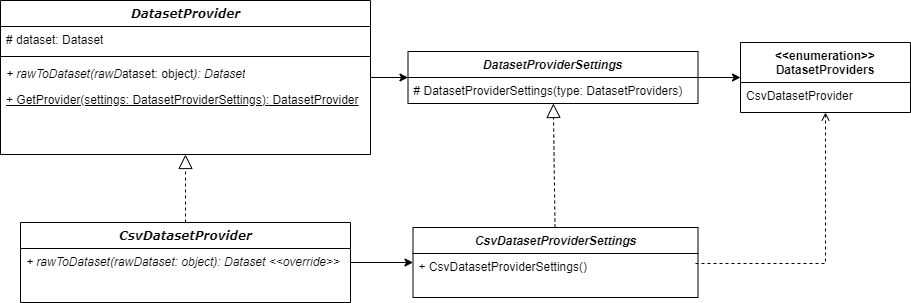
\includegraphics[width=\textwidth]{dataset_provider.png}
\caption{Triedny diagram: načítanie dát zo súbor s príponou .csv}
\end{figure} \\
Samotné spracovanie datasetu prebieha v 2 krokoch:
\begin{enumerate}
\item vytvorenie inštancie potomka triedy \textbf{DatasetProvider}
\item spracovanie datasetu zavolaním abstraktnej metódy \textbf{rawToDataset()}
\end{enumerate}

\subsection{Analytics.Measures}
Táto knižnica poskytuje metódy nutné pre porovnanie dvoch objektov datasetu. 
\begin{figure}[H]
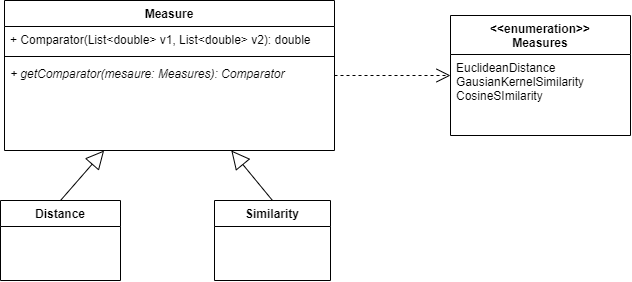
\includegraphics[width=\textwidth]{measure.png}
\caption{Triedny diagram: kľúčové triedy pre výpočet podobnosti a vzdialenosti}
\end{figure} \\
Knižnica využíva konštrukciu jazyka csharp s názvom delegát \cite{delegates}. Delegát je dátova štruktúra reprezentujúca referenciu na funkciu. Delegát ma striktne určený počet a typ parametrov a návratovú hodnotu.

Delegát s názvom \textbf{Comparator} očakáva na vstupe 2 vektory rovnakej dimenzie. Výstupom je podobnosť alebo vzdialenosť. Podobnosť ktorá bude použitá je určená parametrom metódy \textbf{getComparator()}.

\subsection{Analytics.NetworkConstruction}
\label{cap:network_construction}
Pre transformáciu datsetu z vektorovej formy, do formy grafu boli implementované 4 algoritmy:
\begin{itemize}
\item k-NN + $\epsilon-$radius
\item LRNet
\item NNN
\item ErdosRenyi
\end{itemize}

\begin{figure}[H]
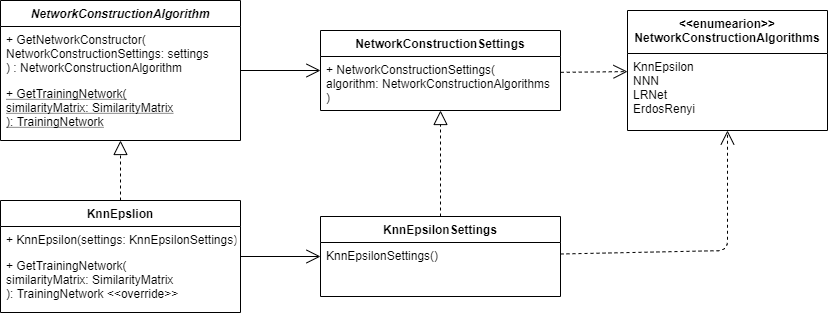
\includegraphics[width=\textwidth]{construction.png}
\caption{Triedny diagram: prevod vektorových dát na sieť pomocou algoritmu kNN + $\epsilon-radius$}
\end{figure} \\

Podobne ako pri spracovaní datasetu, generické rozhranie definuje tovnárnesku metódu \textbf{GetNetworkConstructor()} pre vytvorenie inštancie triedy zodpovednej za transformáciu. Nad vytvorenou inštanciou je možné zavolať abstraktnú metódu \textbf{GetTrainingNetwork()} ktorej výstupom je inštancia triedy TrainingNetwork.

Trieda \textbf{TrainingNetwork} je abstrakcia nad štandardnou implementáciu viacrozmerného poľa jazyka C\#. Táto trieda obsahuje okrem siete uloženej vo forme matici súslednosti aj referenciu na \textit{Comparator}, funkciu použitiu pre zostavenie matice súslednosti. Ďalšiu dôležitou súčasťou je mapovanie Identifikátora objektu datasetu na záznam v matici susednosti. Mapovanie je realizované dátovou štruktúrou \textit{Dictionary<int, Datarow>} kde kľuč je riadok matice a hodnota je zodpovedajúci objekt datasetu. 
Mapovanie je dôležité predovšetkým ak je graf produkovaný touto knižnicou použitý pri kros-validácii, kde je z datasetu vygenerovaných niekoľko sieti z rôznych podmnožín objektov ktoré sú náhodne zoradené. Alternatívne riešenie implementácie by mohlo byť použiť referencii na objekty namiesto ich identifikátorov. Toto riešenie prináša zníženie potrebného výkonu pre operácie s maticami a preto nebolo implementované.

Algoritmus KNN + $\epsilon-$radius pri nastavení parametru k = 0  funguje ako základný $\epsilon-$radius algoritmus rovnako ako pri nastavení $\epsilon$ = 0 algoritmus funguje ako algoritmus k-NN.

Algoritmus ErdosRenyi generuje náhodný model siete \cite{erdos59a} a bol implementovaný ako referenčný algoritmus pre porovnanie výsledkov s ostatnými metódami. 

V priebehu experimentov bola táto knižnica rozšírená o kolekciu tried ktoré slúžia k hľadaniu parametrov algoritmov pre požadovanú hustotu siete. Vzhľadom k faktu že niektoré algoritmy vyžadujú nastavenie viacerých parametrov, existuje viac možností ako danú hustotu dosiahnuť. Hľadanie najlepšej siete pre danú hustotu však reprezentuje problém viacúčelovej optimalizácie ktorá presahuje zameranie tejto práce a preto boli využité jednoduchšie techniky na základe náhody. Bližšie informácie o použití tried je popísane v experimente \ref{exp:density_impact}.

Triedy vytvorené pre hľadanie parametrov pre požadovanú hustotu môžu byť použité aj pre exploračnú  analýzu vďaka implementácií ktorá uchováva pre každý krok hľadania dôležité informácie o sieti ktoré môžu byť použité pri ladení sieti a klasifikačných algoritmov.

Štruktúra dedičnosti tried pre hľadanie hustoty je podobná štruktúre tried pre samotný prevod. Základom je abstraktná trieda \textbf{DensityDiscoverer} ktorá definuje jednu abstraktnú metódu s názvom \textbf{Find()} a parametrom reprezentovaným abstraktnou triedou \textbf{DensityDiscovererSettings}. Výstupom je pole objektov typu \textbf{DensityMemento}. Pre každý algoritmus sú vytvorene 3 triedy ktoré dedia z vyššie uvedených tried a obsahujú implementáciu špecifickú pre daný algoritmus.

\subsection{Analytics.NetworkClassification}
Podobne ako pri spracovaní datasetu alebo konštrukcii siete, najskôr bola vytvorená generická kolekcia tried definujúca rozhranie a následne bol implementovaný algoritmus Ease of Access.
\begin{figure}[H]
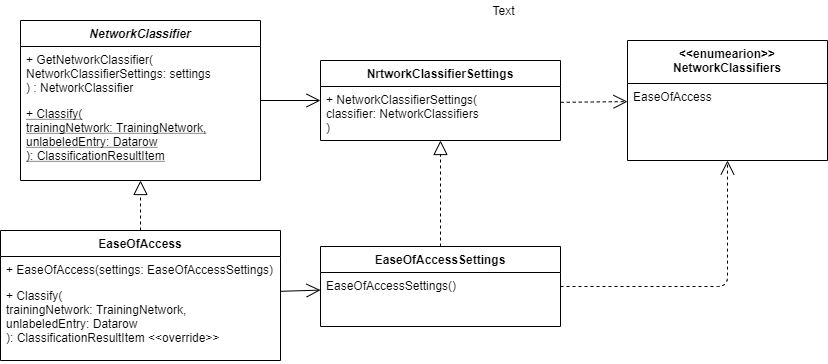
\includegraphics[width=\textwidth]{classificator.png}
\caption{Triedny diagram: klasifikácia pomocou algoritmu Ease of Access }
\end{figure} \\
Klasifikátor očakáva na vstupe sieť ktorá bola zostrojená z označkovaných objektov datasetu a neoznačkovaný objekt. Výstupom algoritmu je inštancia triedy ClassificationResultItem. \\
\textbf{ClassificationResultItem} obsahuje výsledok klasifikácie, referenciu na neoznačkovaný objekt, a kolekciu objektov z ktorých bola výsledná trieda propagovaná.

Knižnica ďalej obsahuje triedu \textbf{Classification}.
Verejne rozhranie tejto triedy je tvorené 2 metódami. \\
Metoda \textbf{ClassifyOne} očakáva na vstupe id objektu nad ktorým ma previesť klasifikáciu. Výstupom tej metódy je ClassificationResultItem. \\
Metoda \textbf{ClassifiyMany} je bezparametrická a slúži na k-násobnú kros-validáciu tréningovej siete. \\
Kros-validácia prebieha v \textit{n} iteráciách V každej iterácii je dataset rozdelený do \textit{k} podmnožín. Prvky podmnožiny sú volené náhodne, pričom je zachovaná rovnomerná distribúcia tried, ktorá je dosiahnutá algoritmom round-robin.\\
Výstupom tejto metódy je \textbf{ClassificationReport}.

\subsection{Aplikácia}
Aplikácia je implementovaná v jazyku .NET Core a opiera sa o architektúru client-server. Na serverovej časti bolo vytvorené WEB API, pre ktoré bol požitý framework ASP.NET Core 3.1. Klient bol implementovaný ako Angular 9 aplikácia. \\

\subsubsection{Spracovanie datasetu}
Prvým krokom klasifikácie je voľba datasetu. Za týmto účelom bol vytvorený formulár pre nahranie datasetu vo forme súboru s príponou \textit{.csv}.
\begin{figure}[H]
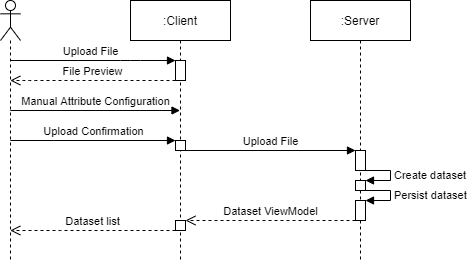
\includegraphics[width=\textwidth]{uploadDataset.png}
\caption{Sekvenčný diagram: nahranie datasetu}
\end{figure} \\
Po otvorení formulára užívateľ najskôr zvolí cestu k súbor ktorý chce nahrať. Klient následne spracuje súbor a zobrazí náhľad dát. Súčasťou spracovania súboru je okrem detekcie základnej štruktúry súboru aj detekcia typu niektorých atribútov. Následujúce typy atribútov sú detegované automaticky na základe názvu stĺpca:
\begin{itemize}
\item \textbf{id} - identifikátor objektu
\item \textbf{label/name} - štítok objektu
\item \textbf{class/group} - trieda objektu
\end{itemize}
Ak názov stĺpca nezodpovedá vyššie uvedeným  typom použije sa prednastavený typ \textbf{attribute}, identifikujúci atribút objektu ktorý sa ďalej využíva pre výpočet podobnosti alebo vzdialenosti. \\
Ak súbor neobsahuje hlavičku s názvami stĺpcov, názvy sú vygenerované vo formáte $a = {a0, a1, ..., an}$.
V ďalšom kroku môže užívateľ manuálne zmeniť detegované typy atribútov a potvrdiť spracovanie. Po potvrdení spracovania je súbor spolu s metadatamy odoslaný na server kde je z neho vytvorený dataset ktorý je následne uložený v databáze.  Po spracovaní a uložení datasetu je vytvorený náhľad datasetu, ktorý je odoslaný ako odpoveď klientovi a zobrazený užívateľovi.

\begin{figure}[H]
\centering
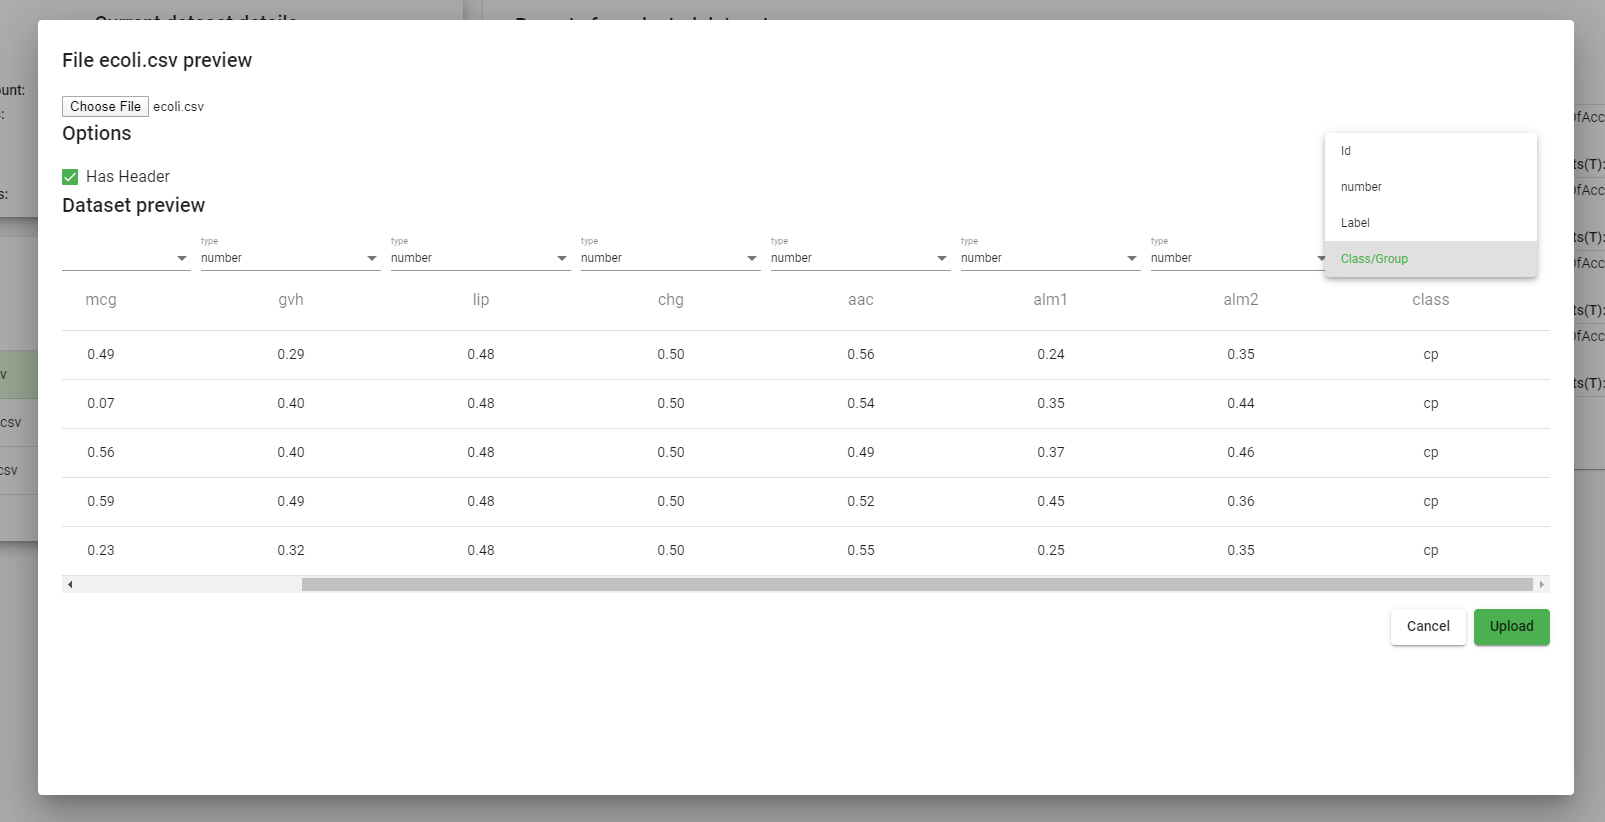
\includegraphics[width=0.75\textwidth]{upload_dataset.PNG}
\caption{Ukážka aplikácie: formulár pre nahranie datasetu}
\end{figure} 

\subsubsection{Domovská stránka}
Po načítaní aplikácie je užívateľovi zobrazený zoznam uložených datasetov. Po kliknutí na dataset sa zobrazí jeho detail a uložene výsledky klasifikácii nad týmto datasetom.

\begin{figure}[H]
\centering
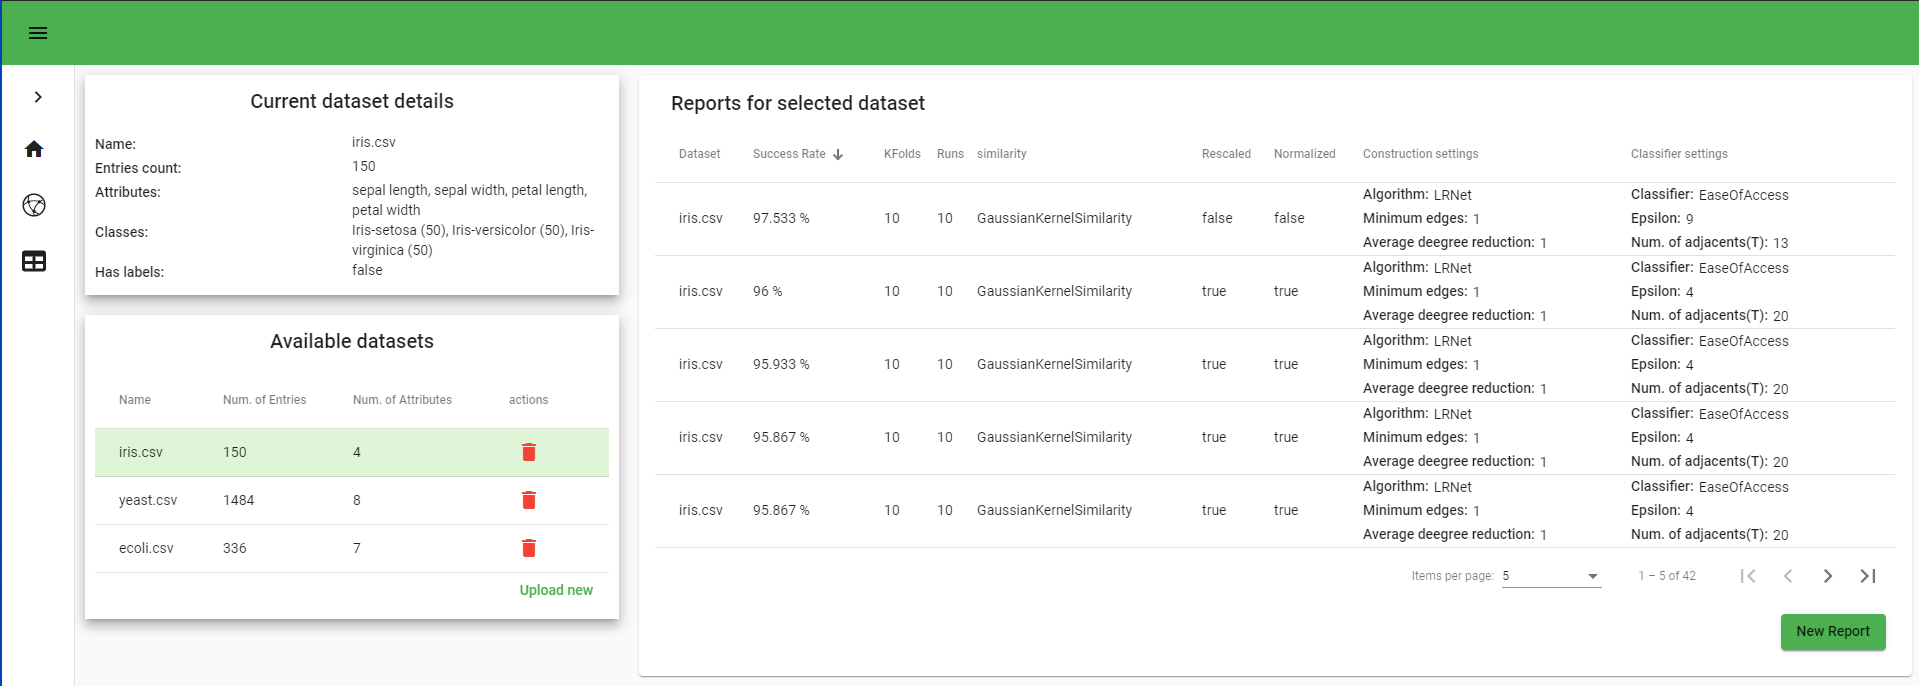
\includegraphics[width=\textwidth]{dataset_preview.PNG} 
\caption{Ukážka aplikácie: domovská stránka}
\end{figure} 


\subsubsection{Vizualizácia siete}
\label{network_visualziation} Pre potreby aplikácie vznikol modul obsahujúci interaktívny model grafu. Vzhľadom k špecifickým požiadavkám aplikácie a nedostatočnej podpory už existujúcich riešení pre interaktívnu prácu s grafom bola zvolená knižnica \textit{d3.js}, ktorá poskytuje množstvo funkcii pre implementáciu požadovanej funkcionality.
\begin{figure}[H]
\centering
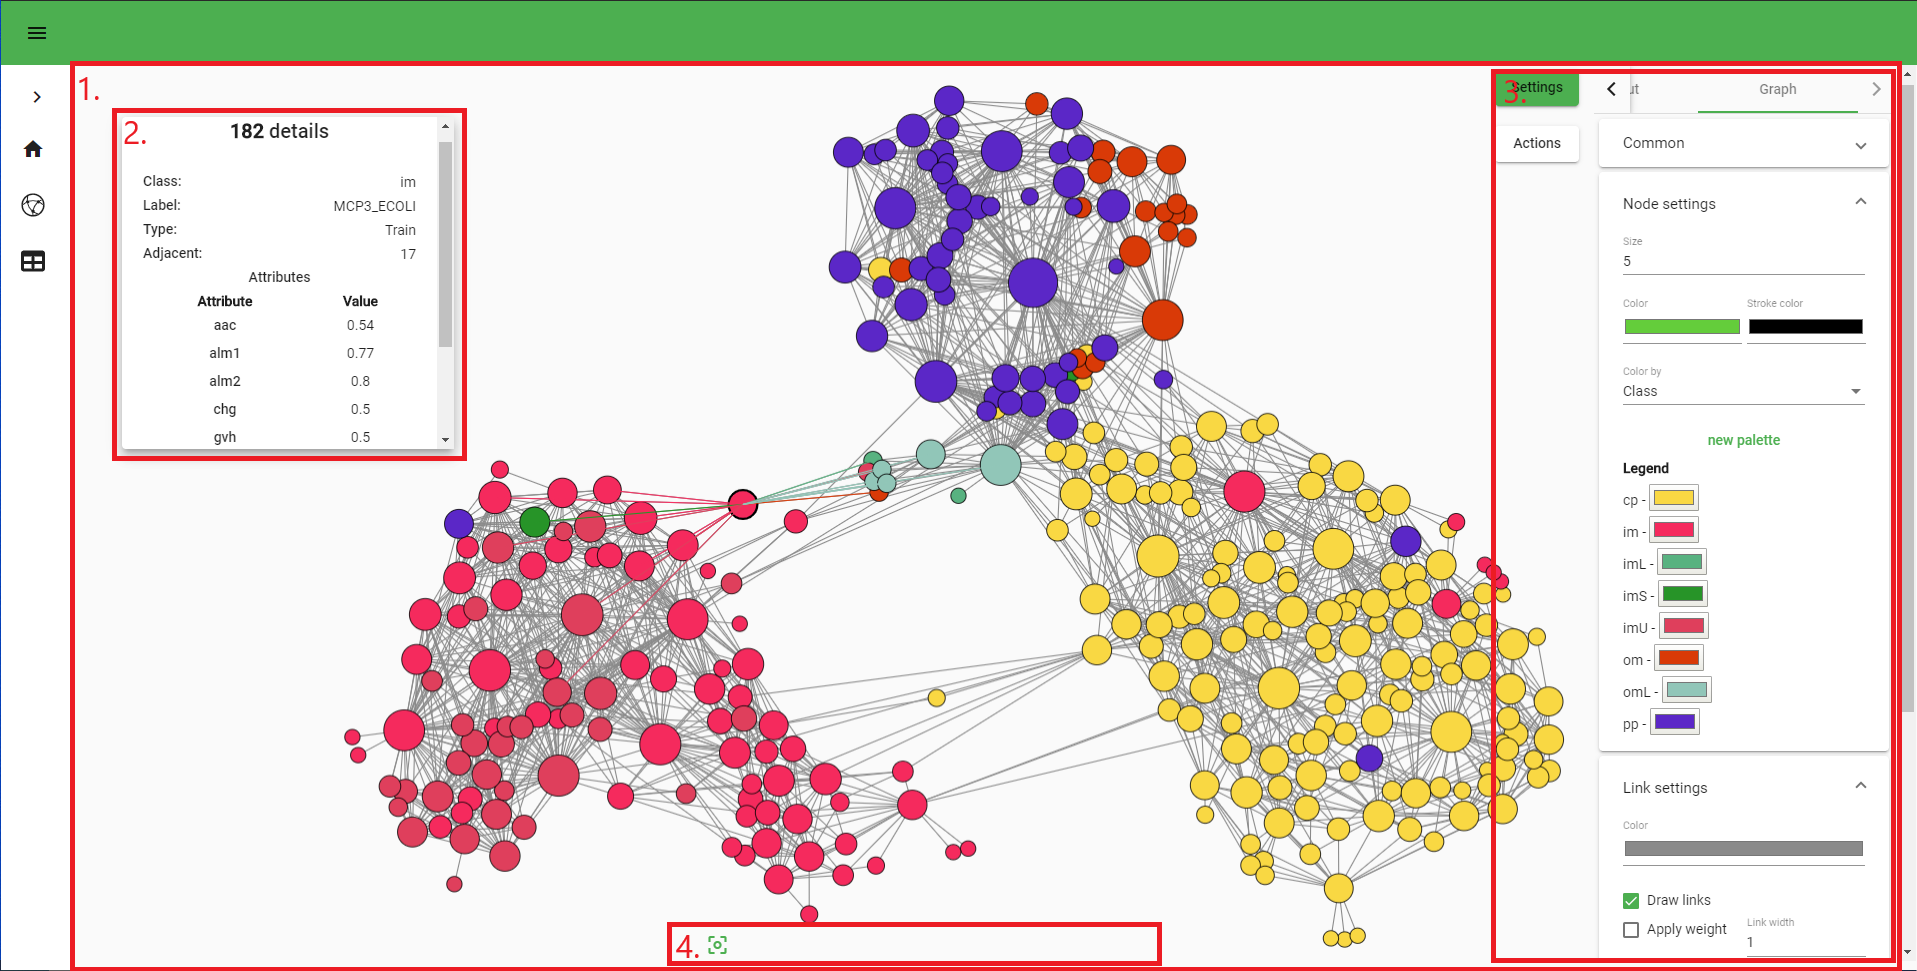
\includegraphics[width=\textwidth]{ecoli_graph_numbers.png}
\caption{Ukážka aplikácie: rozhranie pre vizualizáciu siete}
\label{pic:graph_vizualization}
\end{figure} 
Na obrázku \ref{pic:graph_vizualization} môžeme vidieť 4 zvýraznené komponenty.
\begin{enumerate}
    \item \textbf{Graf} - hlavná komponenta obsahujúca sieť vykreslenú pomocou HTML elementu s názvom \textit{<canvas>}. Medzi implementované prvky interakcie patrí:
\begin{itemize}
\item \textbf{zoom} - približovanie a odďaľovanie grafu
\item \textbf{pan} - posúvanie grafu
\item \textbf{drag} - presúvanie vrcholov
\item \textbf{select} - zvolenie a zvýraznenie vrcholu
\end{itemize}
\item \textbf{Detail vrcholu} - komponenta zobrazujúca detaily zvoleného vrcholu
\item \textbf{Postranne menu} - komponenta obsahuje 2 logické celky.
    \begin{enumerate}
        \item \textbf{settings} - menu nastavenia grafu, ktoré je ďalej rozdelené na 
        \begin{enumerate}
            \item nastavenia vizuálnych vlastnosti grafu
            \item nastavenia rozloženia grafu 
        \end{enumerate}
        \item \textbf{actions} - nepovinne menu obsahujúce funkcionalitu špecifickú pre použitie grafu. Táto konštrukcia umožňuje dodať funkcionalitu pre rôzne užívateľské scenáre ako napríklad ladenie grafu, kde menu \textbf{actions} obsahuje komponentu pre generovanie tréningovej siete.
    \end{enumerate}
\item \textbf{Menu s rýchlymi akciami} - táto komponenta slúži ako kontajner pre ďalšiu interakciu s grafom a obsahuje jednu funkciu ktorá resetuje pohľad a priblíženie na prednastavené hodnoty. 

Okrem komponent slúžiacich na vizualizáciu siete modul obsahuje  aj komponentu pre rozloženie grafu realizovanú pomocou služby. Rozloženie grafu, tiež známe ako \textbf{layout} prebieha kvôli vypočetnej náročnosti v samostatnom vlákne a nove pozície vrcholov sú priebežne zasielané na hlavné vlákno, pomocou ktorého sú vykreslené. Pokročilé nastavenia algoritmu pre generovanie rozloženia sú prístupné v postrannom menu.
\end{enumerate}


\subsubsection{Ladenie siete}
S využitím modulu pre vizualizáciu a interakciu so sieťou  \ref{network_visualziation} bola implementovaná komponenta pre ladenie siete.
Táto komponenta umožňuje rýchly náhľad na dataset v podobe siete a jej následne ladenie pre použitie na klasifikáciu.


\subsubsection{Ladenie klasifikácie}
Ladenie samotnej klasifikácie prebieha pomocou k-násobnej krížovej validácie. Užívateľ vyplní formulár ktorý je odoslaný na server kde prebehne samotná klasifikácia. Nastavenie klasifikácie môžeme rozdeliť do 4 krokov.
\begin{enumerate}
\item nastavenie podobnosti
\item nastavenie algoritmu pre konštrukciu siete
\item všeobecne nastavenie klasifikácie 
\item nastavenie klasifikačného algoritmu
\end{enumerate}
Na obrázku \ref{pic:classification_settings} môžeme vidieť formulár pre nastavenie klasifikácie pričom vstupy pre nastavenie algoritmu pre konštrukciu siete a nastavenie klasifikačného algoritmu sú zobrazené dynamicky na základe zvoleného algoritmu
\begin{figure}[H]
\centering
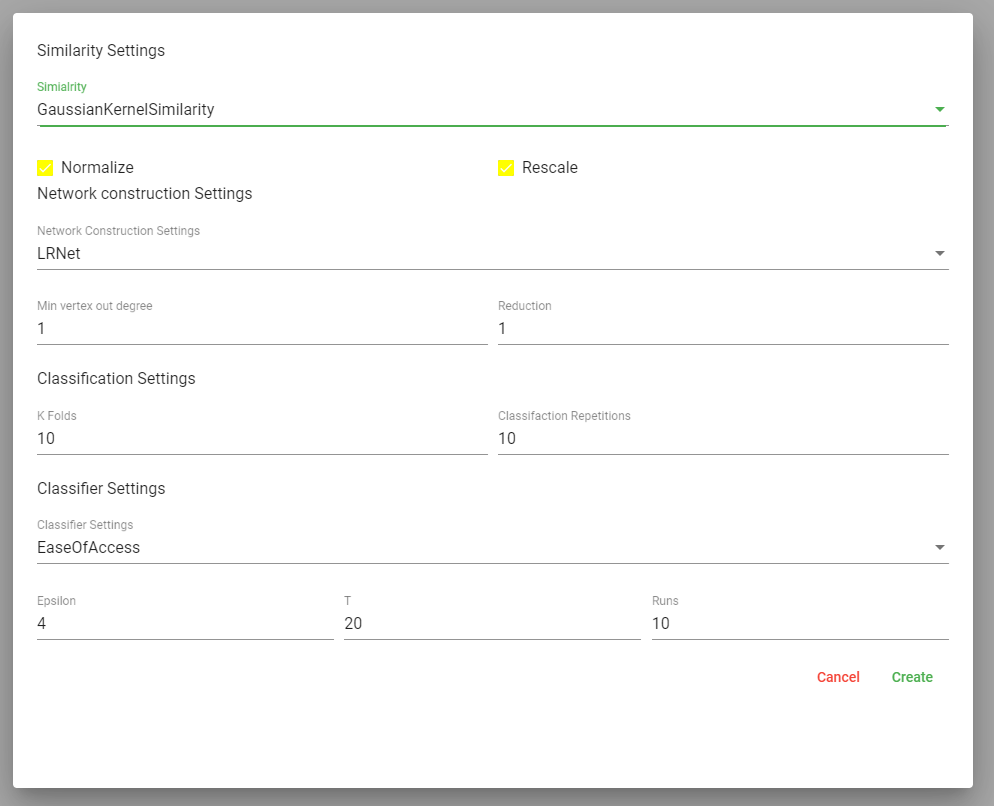
\includegraphics[width=\textwidth]{classification_settings.PNG}
\caption{Ukážka aplikácie: formulár pre nastavenie klasifikácie}
\label{pic:classification_settings}
\end{figure}  \\
Po dokončení klasifikácie je užívateľovi odoslaný výsledok ktorý je následne vizualizovaný. Komponenta pre vizualizáciu výsledku je rozdelená na následujúce čast:
\begin{enumerate}
\item \textbf{Použité nastavenie}
\item \textbf{Výsledok klasifikácie} - okrem výsledku obsahuje rozhranie pre zmenu aktuálne zobrazených detailov.
\item \textbf{Nesprávne klasifikované objekty} - tabuľka obsahujúca počet nesprávnych klasifikácii pre každý objekt.
\item \textbf{Confusion matrix} - zobrazuje maticu kde stĺpce zobrazujú reálnu triedu objektu a riadky predikovanú.
\item \textbf{Použitá sieť} - interaktívny graf s využitím modulu pre vizualizáciu a interakciu so sieťou  \ref{network_visualziation}. Vrcholy testovacích objektov sú v grafe zobrazené ako šedou farbou. Ich okraje sú zelené ak bola predikovaná trieda správna alebo črevné ak bola predikovaná trieda nesprávna. Po kliknutí na testovací objekt sú zobrazené hrany medzi s vrcholmi, ktoré boli použité pre propagáciu triedy.
\end{enumerate}
\begin{figure}[H]
\centering
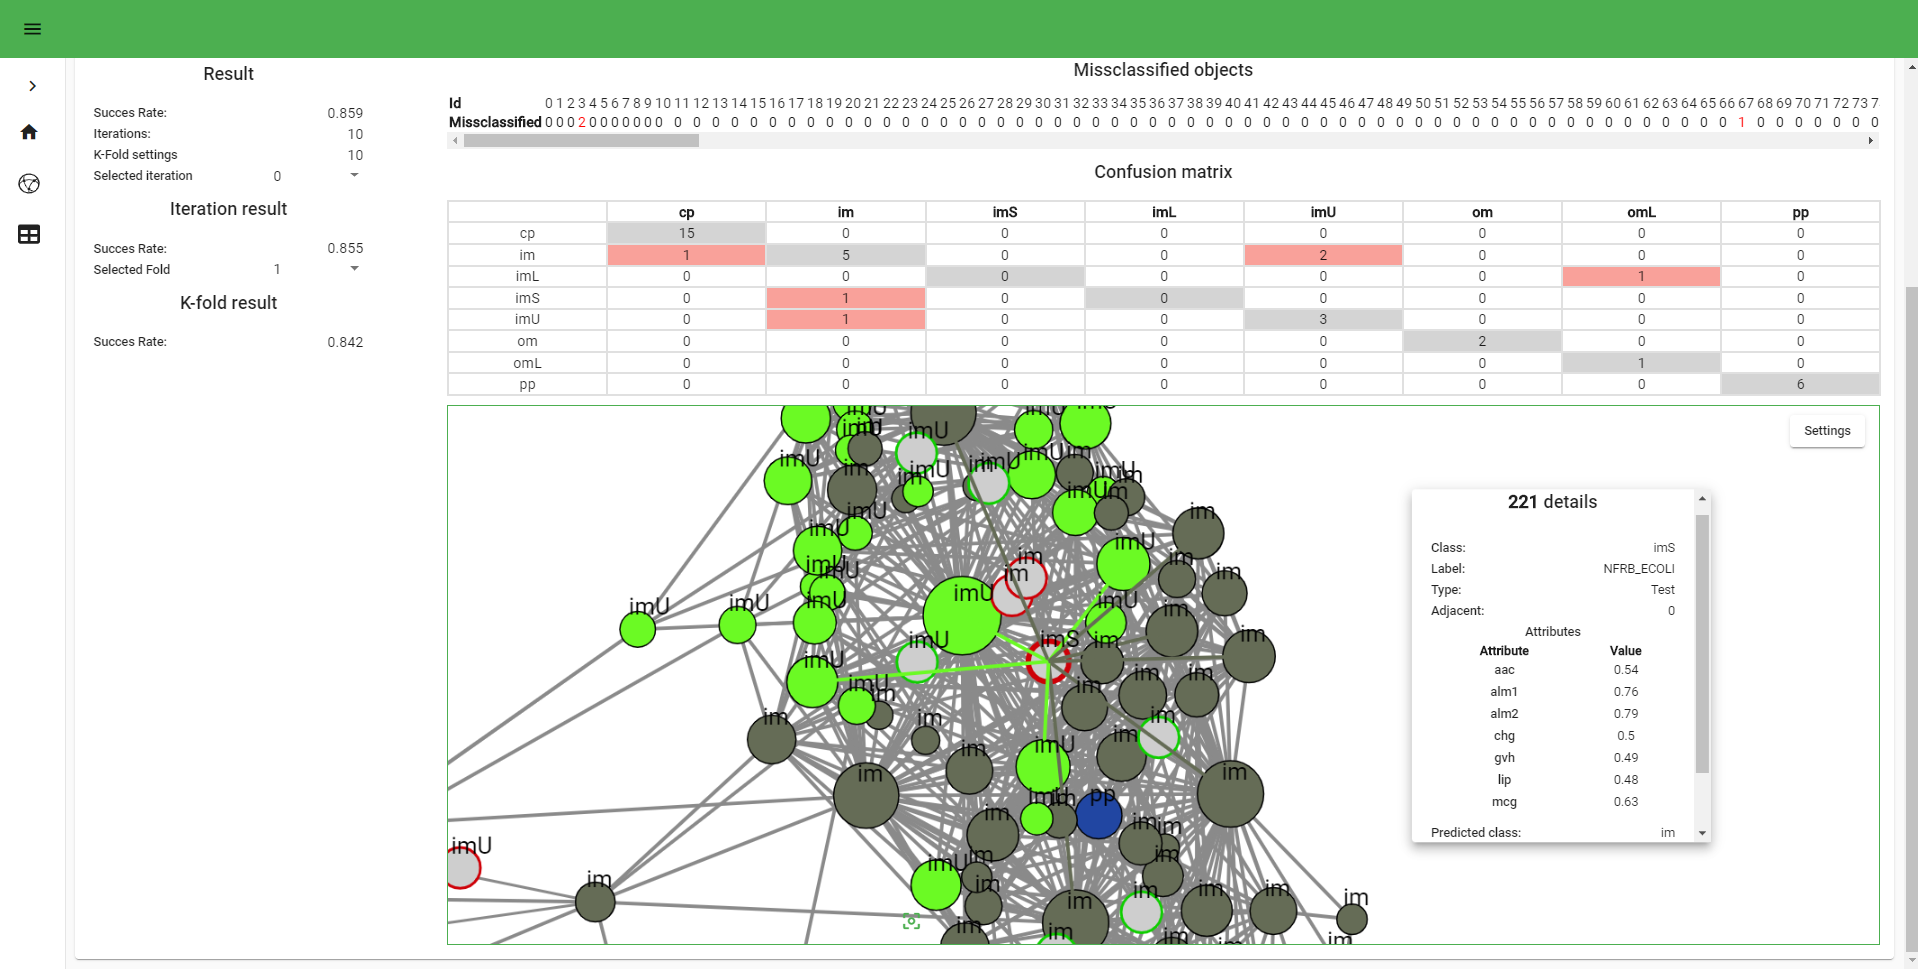
\includegraphics[width=\textwidth]{classification_result.PNG}
\caption{Ukážka aplikácie: rozhranie pre zobrazenie výsledku klasifikácie}
\end{figure} 
        
\section{Experimenty}
Experimenty vykonané v tejto práci sa zameriavajú na porovnanie a vyhodnotenie klasifikácie pomocou sietí. Pre experimenty bolí zvolené algoritmy \textit{Ease of Acces} a algoritmus \textit{Averrage Link Weigth}.

Pre prevod vektorových dát na sieť boli použite algoritmy \textit{kNN + $\epsilon-radius$}, \textit{NNN} z \textit{LRNet} a referenčný algoritmus pre generovanie náhodných sieti \textit{Erdos-Renyi}. Voľba správneho algoritmu pre vytvorenie siete zohráva pri klasifikácii pomocou sieti dôležitú úlohu a preto sú v experimentoch taktiež detailne skúmané. 

Na začiatku tejto kapitoly sú uvedené datasety ktoré boli použité v experimentoch. Datasety boli zvolené z typických datasetov v oblasti klasifikácie, pričom boli preferované datasety s nižším počtom vrcholov čo umožňuje ľahšiu vizualizáciu a nižšiu vypočtovú náročnosť.  Ku každému datasetu boli vytvorené siete pomocou implementovaných algoritmov. Siete boli vytvorené s rovnakou hustotou pre lepšie vizuálne porovnanie.

\subsection{Použité datasety}\label{used_dataset}

\subsubsection{Iris dataset}
Jedná sa asi o najznámejší dataset v oblasti klasifikácie. Vďaka malému počtu pozorovaní rozdelených do 3 rovnako veľkých skupín je tento dataset vhodný na rýchle testovanie algoritmov, vizualizáciu a testovanie predpokladov.

Dataset obsahuje 150 záznamov a 4 atribúty. Záznamy sú rovnomerne rozdelené do troch tried. Jednotlive záznamy predstavujú kvety z rodu Iris a atribúty predstavujú ich proporcie. Na základe proporcii je rastlina zradená do jednej z troch odrôd.\cite{iris}

\begin{figure}[H]
\centering
\begin{subfigure}{0.45\textwidth}
    \centering
    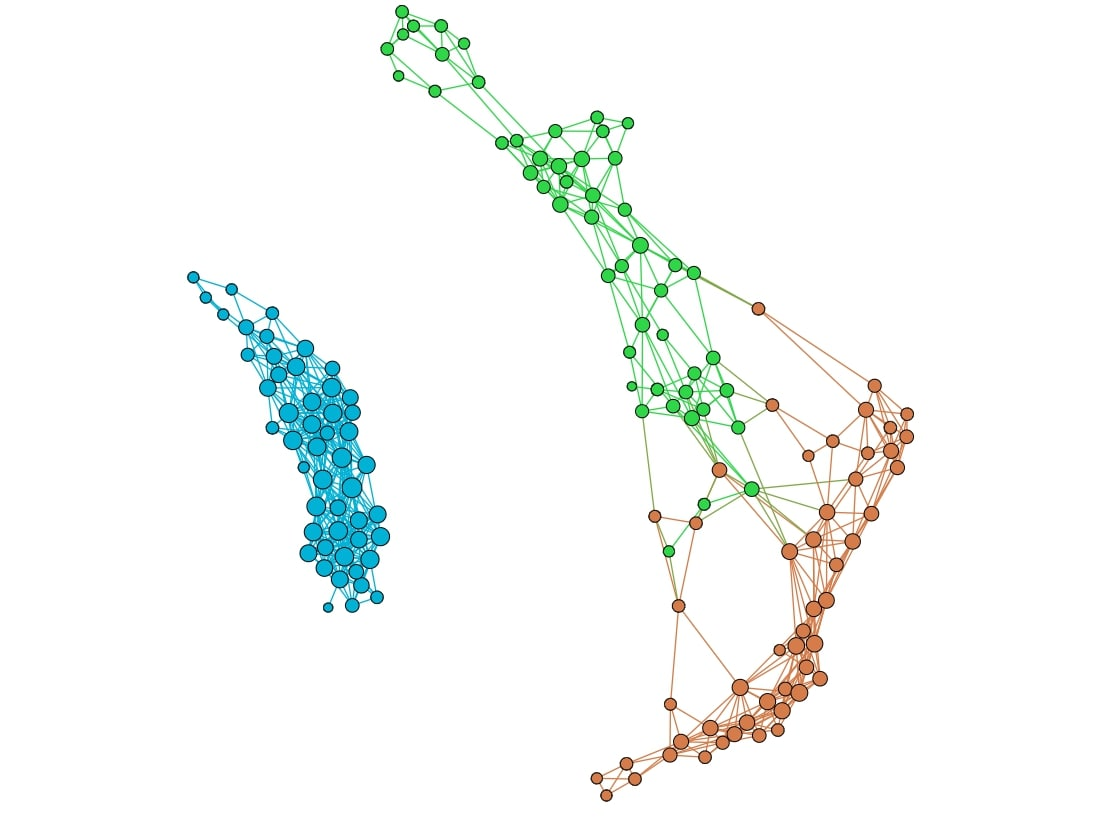
\includegraphics[width=\linewidth, frame]{Graphs/network_iris_knn_epsilon.jpg}
    \caption{kNN + epsilon radius}
    \label{fig:wine_knn_eps}
\end{subfigure}\hfil
\begin{subfigure}{0.45\textwidth}
    \centering
    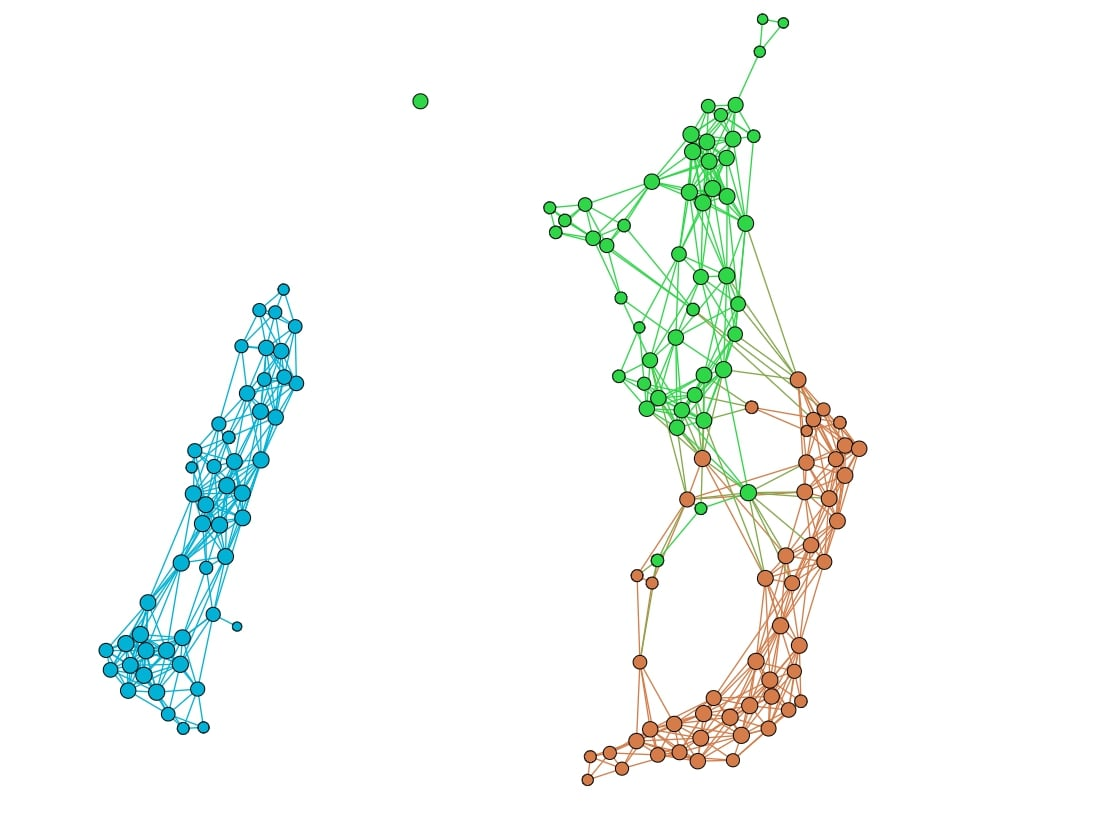
\includegraphics[width=\linewidth, frame]{Graphs/network_iris_nnn.jpg}
    \caption{NNN}
    \label{fig:wine_nnn}
\end{subfigure}
\medskip
\begin{subfigure}{0.45\textwidth}
    \centering
    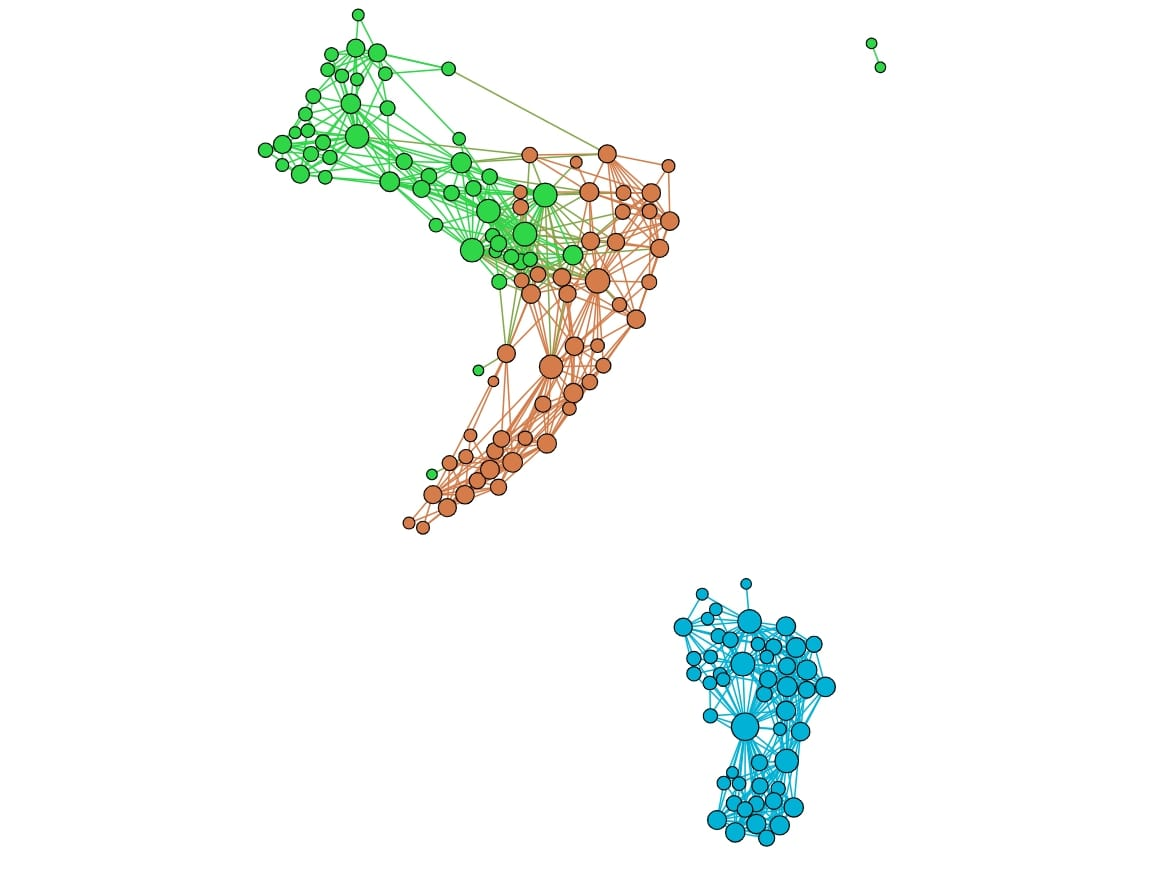
\includegraphics[width=\linewidth, frame]{Graphs/network_iris_lrnet.jpg}
    \caption{LRNet}
    \label{fig:wine_lrnet}
\end{subfigure}\hfil
\begin{subfigure}{0.45\textwidth}
    \centering
    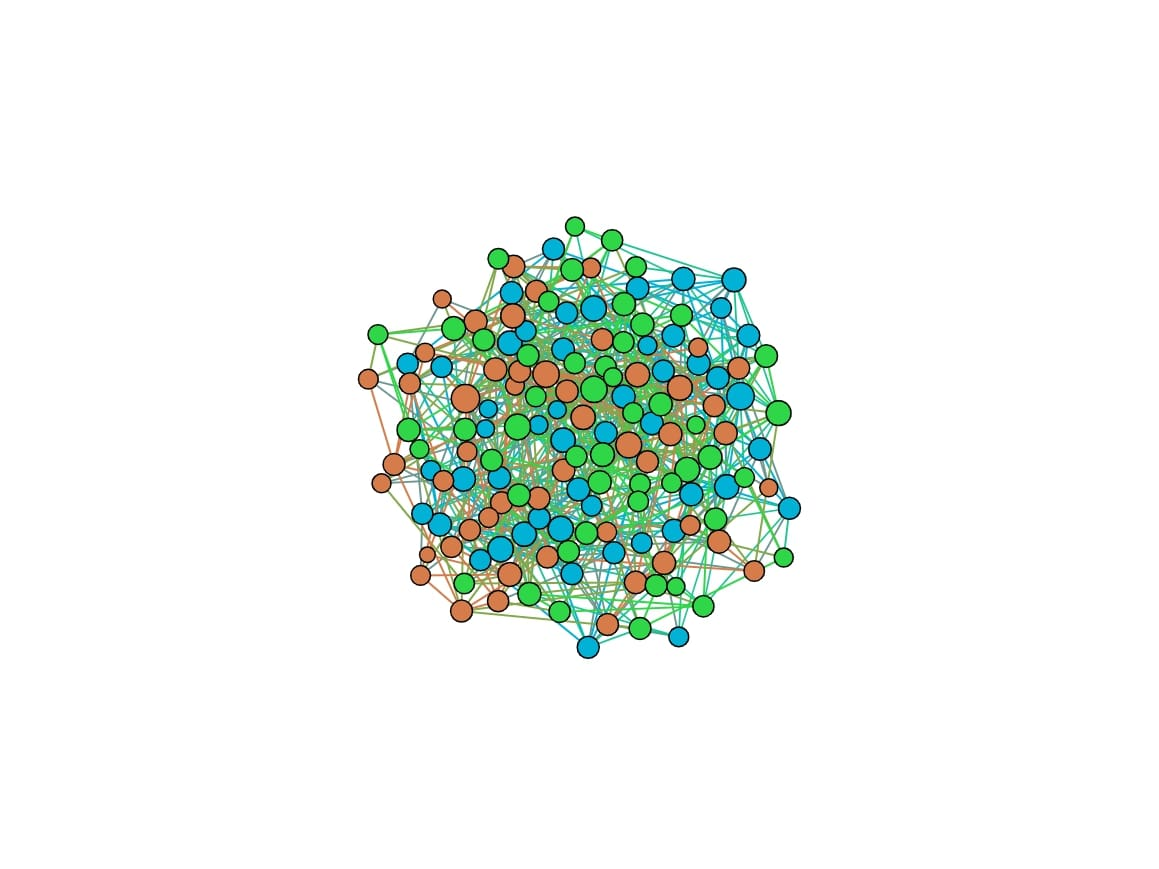
\includegraphics[width=\linewidth, frame]{Graphs/network_iris_erdos_renyi.jpg}
    \caption{Erods Renyi}
    \label{fig:wine_erdos_renyi}
\end{subfigure}
\caption{Siete datasetu Iris}
\label{fig:wine_networks}
\end{figure}


\subsubsection{E.Coli dataset}
Dataset obsahuje 336 meraní proteinových sekvencií baktérie Escherichia coli. U každého merania bolo sledovaných 8 atribútov na základe ktorých bola meraniu priradená 1 z 8 tried reprezentujúca v ktorej časti bunky sa proteín nachádza. \cite{E.Coli}

\begin{figure}[H]
\centering
\begin{subfigure}{0.45\textwidth}
    \centering
    \includegraphics[width=\linewidth, frame]{Graphs/network_ecoli_knn_epsilon.jpg}
    \caption{kNN + epsilon radius}
    \label{fig:wine_knn_eps}
\end{subfigure}\hfil
\begin{subfigure}{0.45\textwidth}
    \centering
    \includegraphics[width=\linewidth, frame]{Graphs/network_ecoli_nnn.jpg}
    \caption{NNN}
    \label{fig:wine_nnn}
\end{subfigure}
\medskip
\begin{subfigure}{0.45\textwidth}
    \centering
    \includegraphics[width=\linewidth, frame]{Graphs/network_ecoli_lrnet.jpg}
    \caption{LRNet}
    \label{fig:wine_lrnet}
\end{subfigure}\hfil
\begin{subfigure}{0.45\textwidth}
    \centering
    \includegraphics[width=\linewidth, frame]{Graphs/network_ecoli_erdos_renyi.jpg}
    \caption{Erods Renyi}
    \label{fig:wine_erdos_renyi}
\end{subfigure}
\caption{Siete datasetu E.Coli}
\label{fig:wine_networks}
\end{figure}

\subsubsection{Glass dataset}
Dataset obsahuje 214 meraní vlastnosti skla. Pri každom zázname bolo meraných 9 vlastnosti na základe ktorých bol určený  1 zo 7 tipov skla. \cite{glass}

\begin{figure}[H]
\centering
\begin{subfigure}{0.45\textwidth}
    \centering
    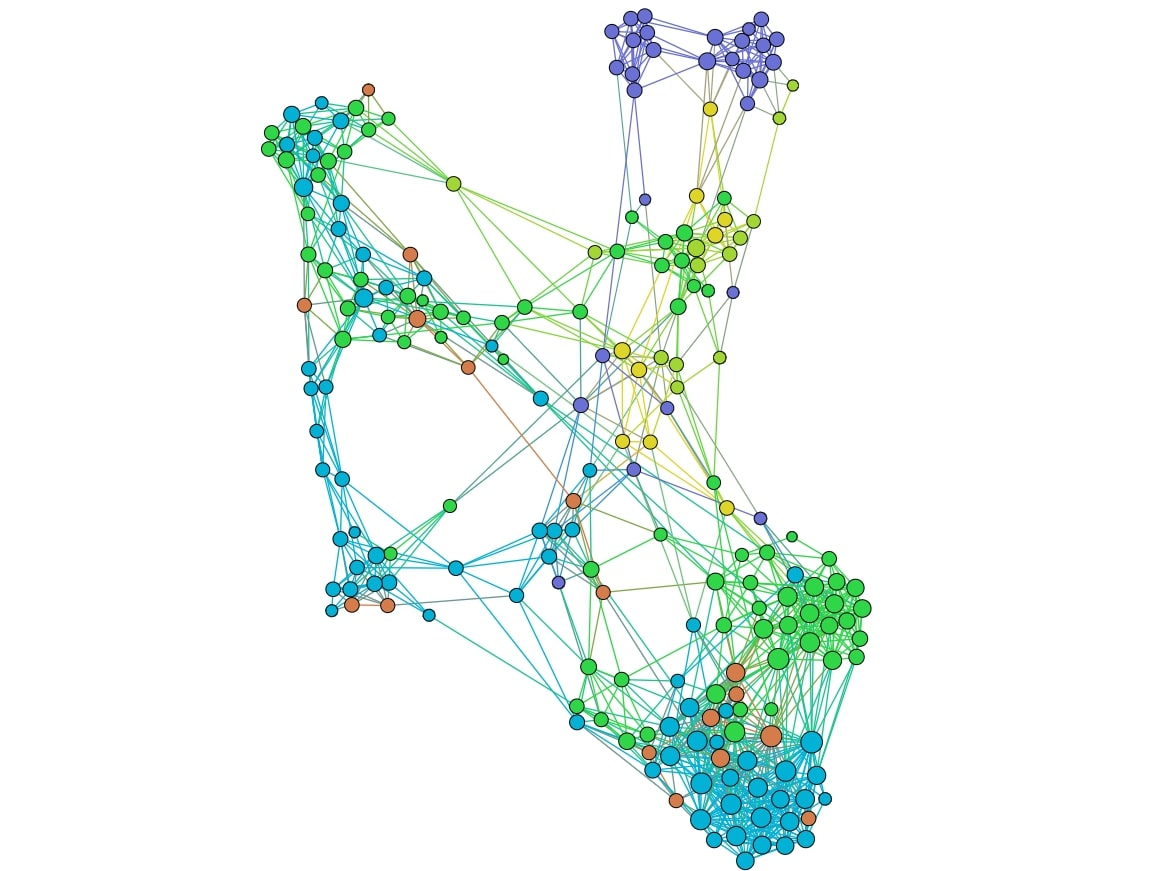
\includegraphics[width=\linewidth, frame]{Graphs/network_glass_knn_epsilon.jpg}
    \caption{kNN + epsilon radius}
    \label{fig:wine_knn_eps}
\end{subfigure}\hfil
\begin{subfigure}{0.45\textwidth}
    \centering
    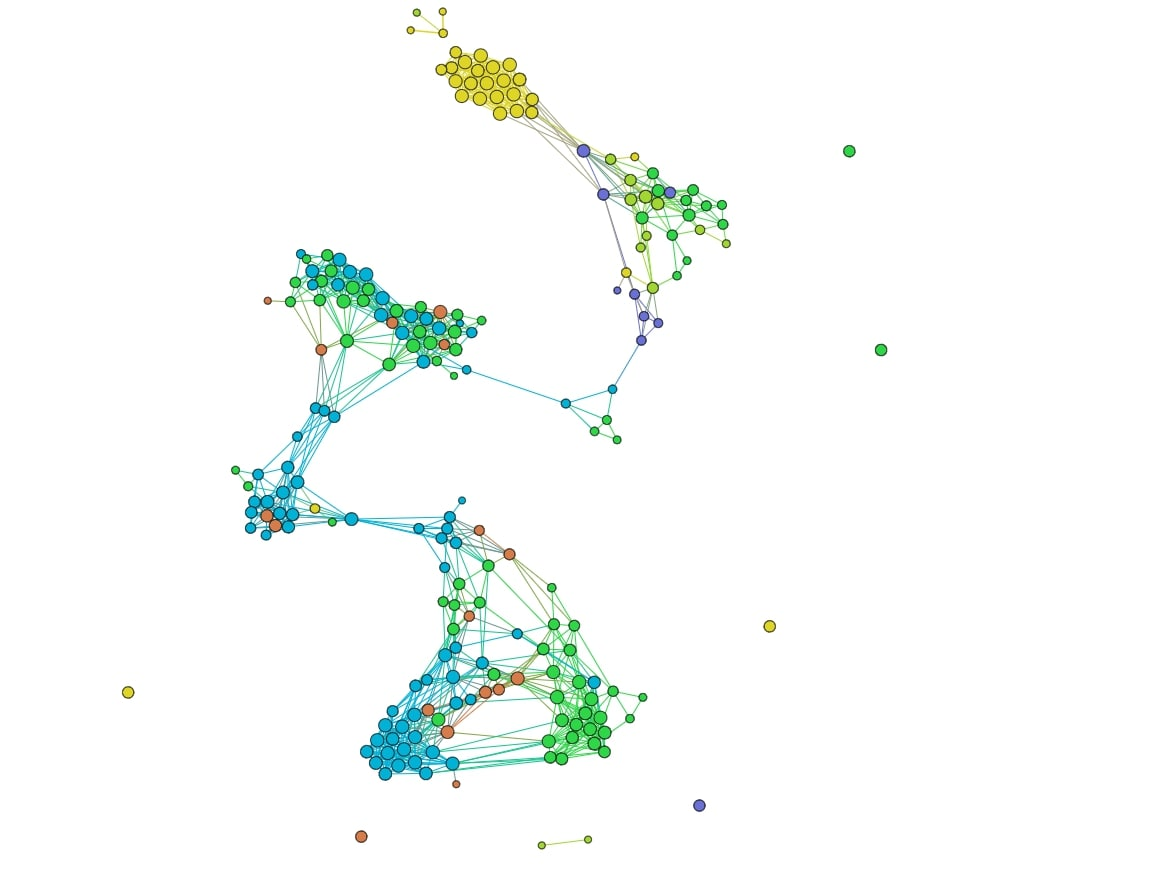
\includegraphics[width=\linewidth, frame]{Graphs/network_glass_nnn.jpg}
    \caption{NNN}
    \label{fig:wine_nnn}
\end{subfigure}
\medskip
\begin{subfigure}{0.45\textwidth}
    \centering
    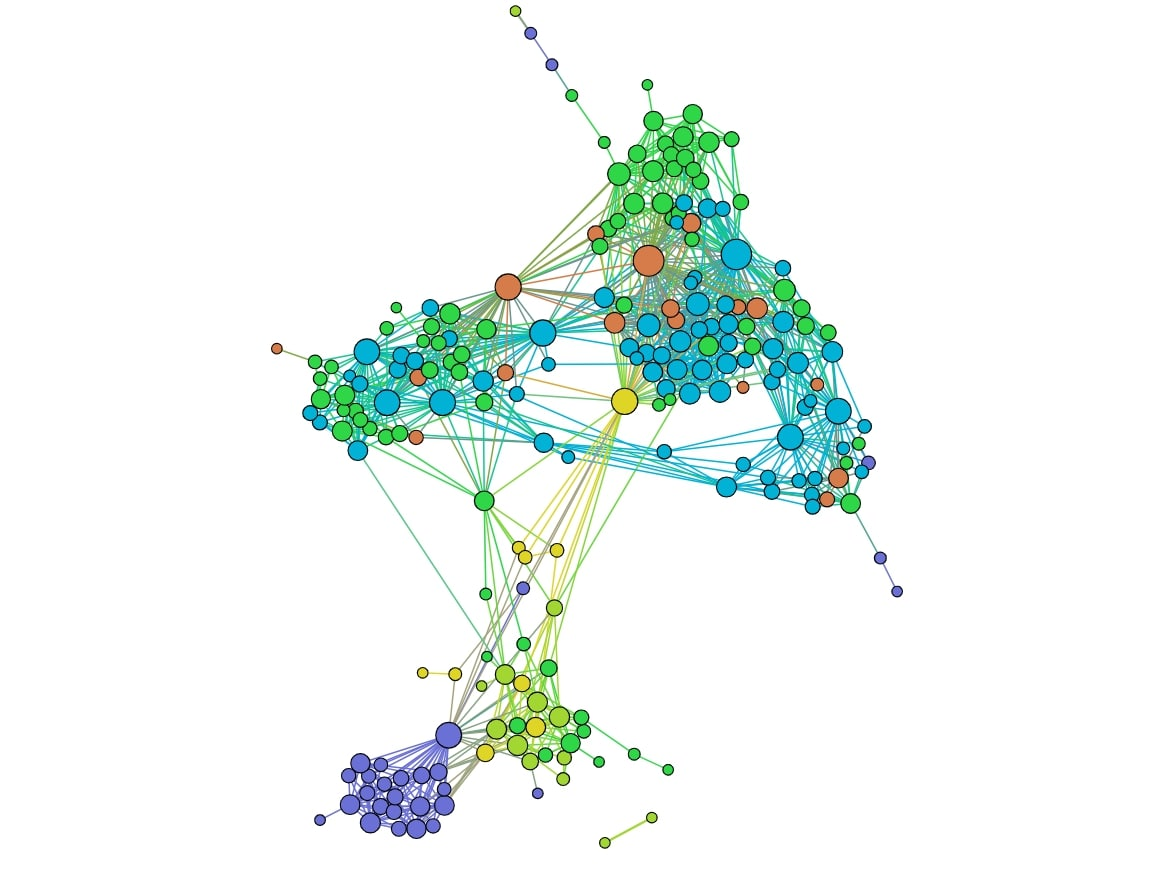
\includegraphics[width=\linewidth, frame]{Graphs/network_glass_lrnet.jpg}
    \caption{LRNet}
    \label{fig:wine_lrnet}
\end{subfigure}\hfil
\begin{subfigure}{0.45\textwidth}
    \centering
    \includegraphics[width=\linewidth, frame]{Graphs/network_glass_erdos_renyi.jpg}
    \caption{Erods Renyi}
    \label{fig:wine_erdos_renyi}
\end{subfigure}
\caption{Siete datasetu Glass}
\label{fig:wine_networks}
\end{figure}

\subsubsection{Wine red dataset}
Dataset obsahuje merania kvality červeného vína.Na základe 11 vlastnosti vína je určená jeho kvalita od 0 do 10. dataset je tvorený 1599 záznamami. Počtom vlastnosti, záznamov a splývajúcimi triedami tento dataset predstavuje zaujímavý cieľ v oblasti klasifikácie. \cite{wine}

\begin{figure}[H]
\centering
\begin{subfigure}{0.45\textwidth}
    \centering
    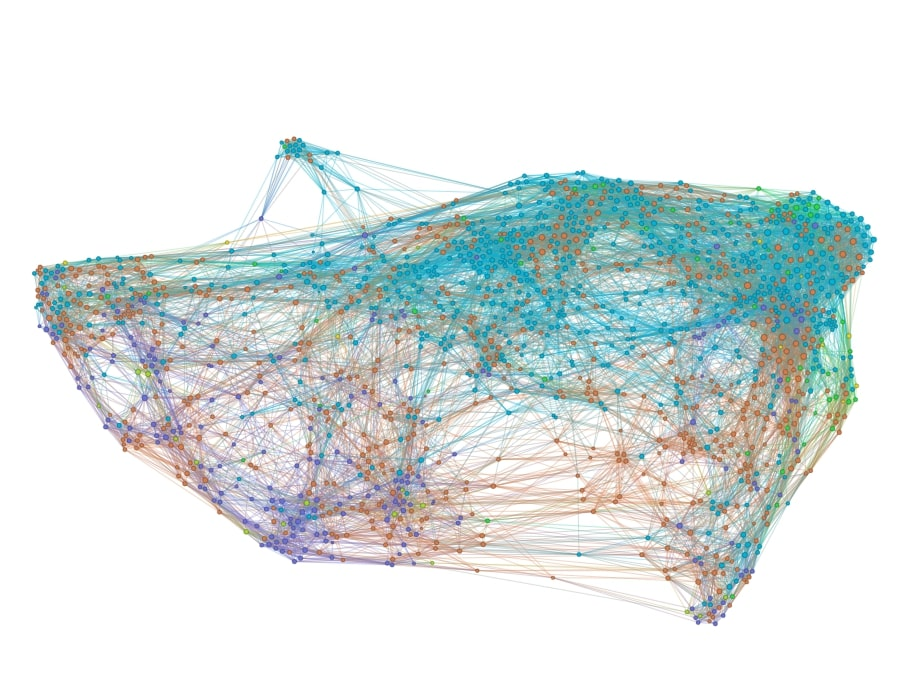
\includegraphics[width=\linewidth, frame]{Graphs/network_wine_red_knn_epsilon.jpg}
    \caption{kNN + epsilon radius}
    \label{fig:wine_knn_eps}
\end{subfigure}\hfil
\begin{subfigure}{0.45\textwidth}
    \centering
    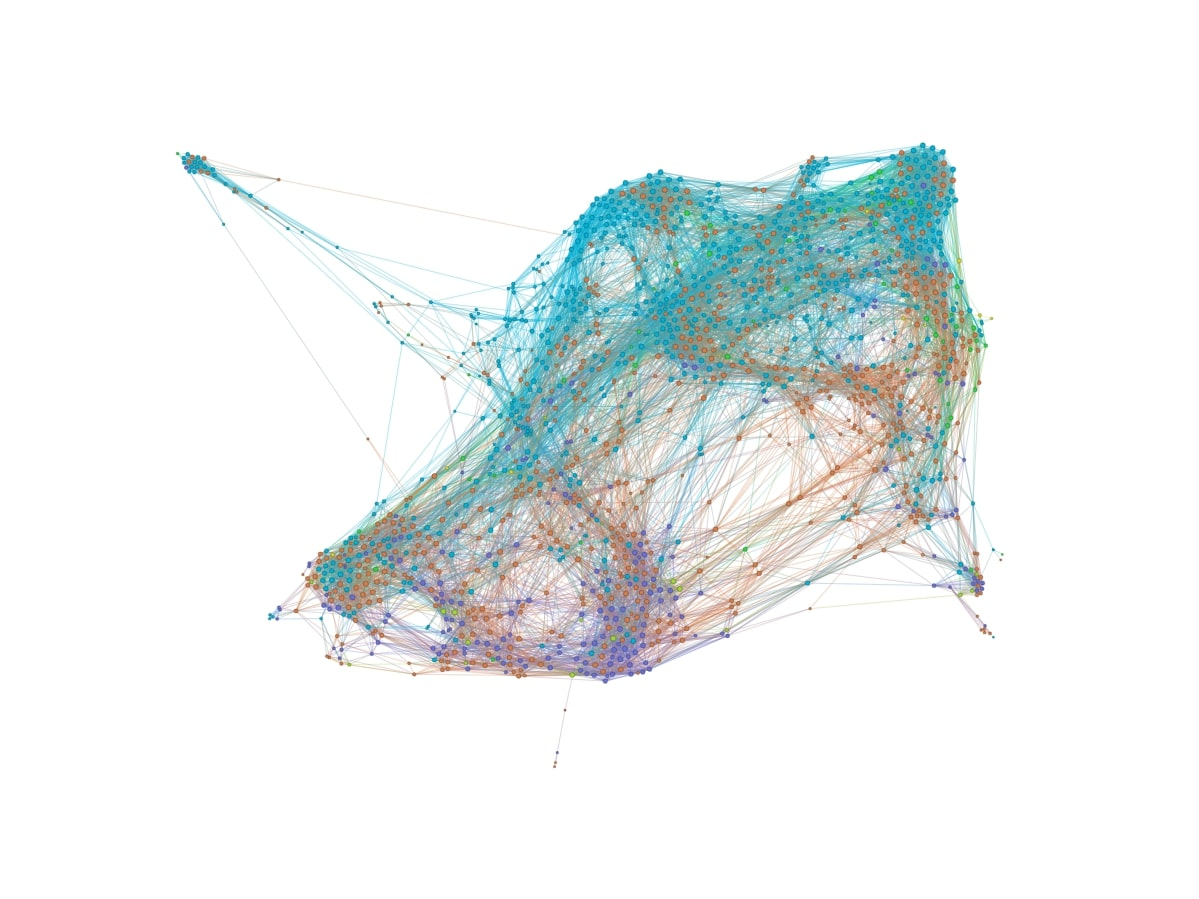
\includegraphics[width=\linewidth, frame]{Graphs/network_wine_red_nnn.jpg}
    \caption{NNN}
    \label{fig:wine_nnn}
\end{subfigure}
\medskip
\begin{subfigure}{0.45\textwidth}
    \centering
    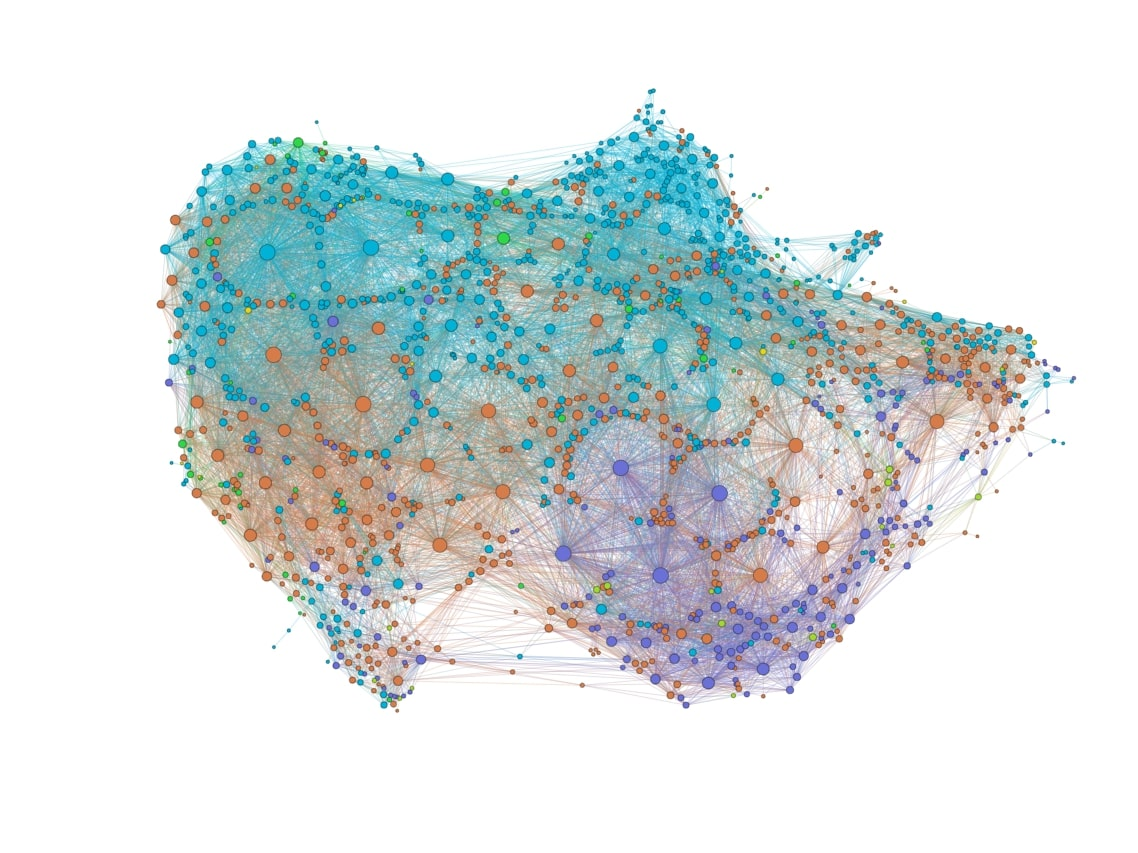
\includegraphics[width=\linewidth, frame]{Graphs/network_wine_red_lrnet.jpg}
    \caption{LRNet}
    \label{fig:wine_lrnet}
\end{subfigure}\hfil
\begin{subfigure}{0.45\textwidth}
    \centering
    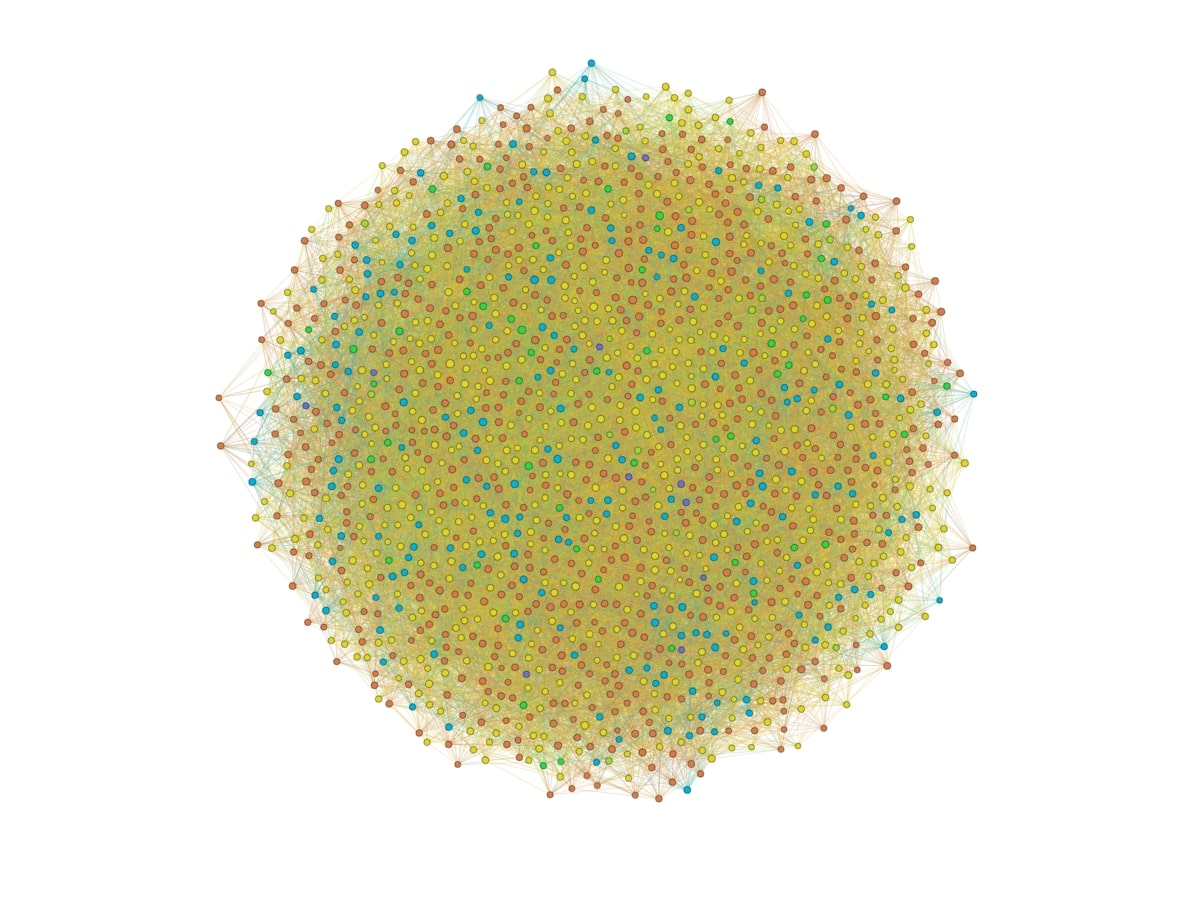
\includegraphics[width=\linewidth, frame]{Graphs/network_wine_red_erdos_renyi.jpg}
    \caption{Erods Renyi}
    \label{fig:wine_erdos_renyi}
\end{subfigure}
\caption{Siete datasetu Wine red}
\label{fig:wine_networks}
\end{figure}

\subsubsection{Vehicle dataset}
Dataset obsahuje 4 triedy automobilov ktorých tvar je zakódovaný do 17 atribútov.\cite{vehicle}
\begin{figure}[H]
\centering
\begin{subfigure}{0.45\textwidth}
    \centering
    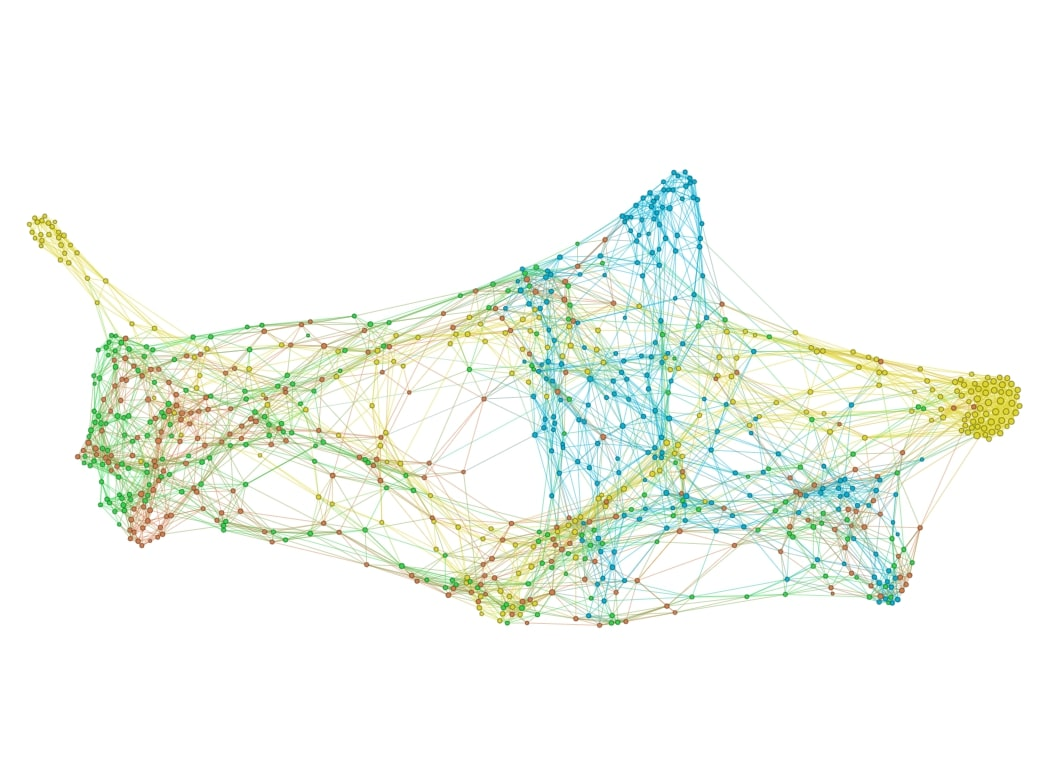
\includegraphics[width=\linewidth, frame]{Graphs/network_vehicle_knn_epsilon.jpg}
    \caption{kNN + epsilon radius}
    \label{fig:wine_knn_eps}
\end{subfigure}\hfil
\begin{subfigure}{0.45\textwidth}
    \centering
    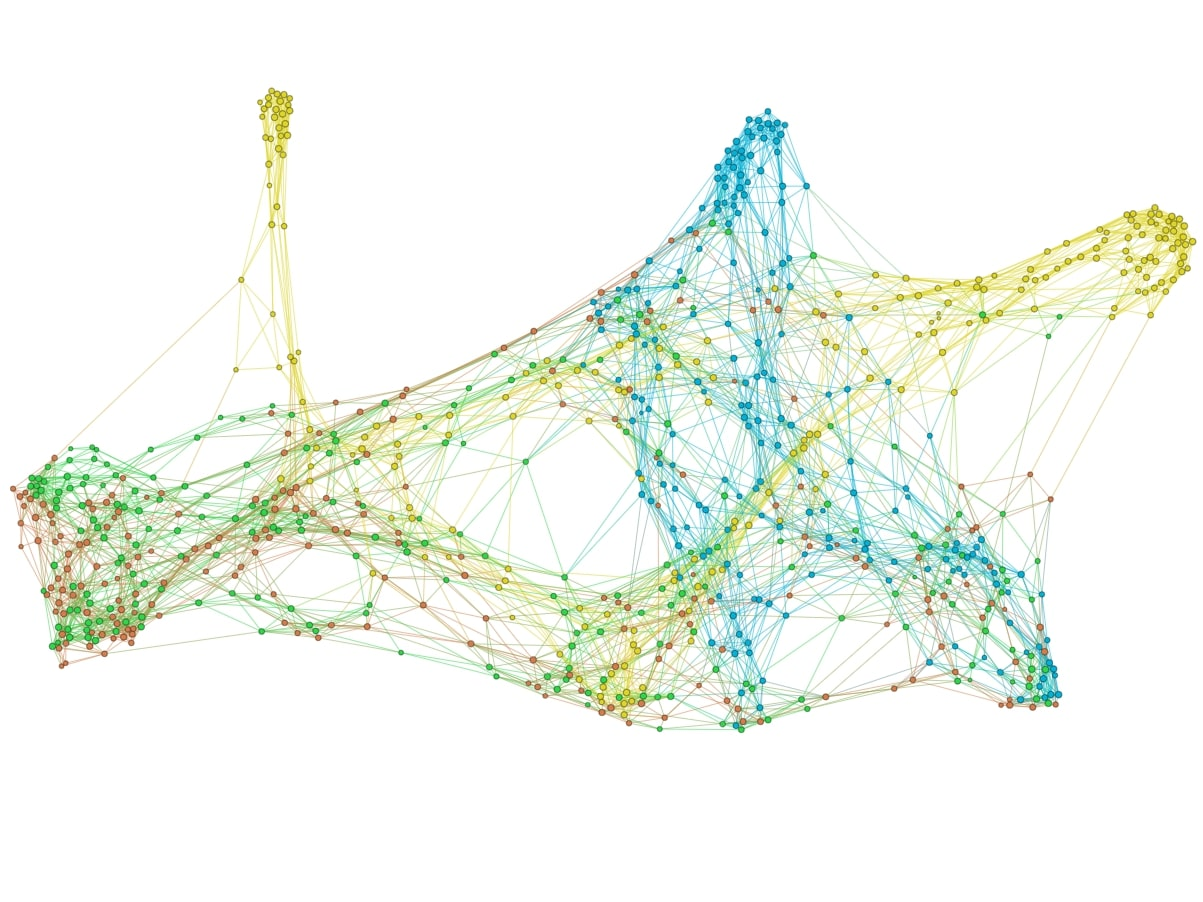
\includegraphics[width=\linewidth, frame]{Graphs/network_vehicle_nnn.jpg}
    \caption{NNN}
    \label{fig:wine_nnn}
\end{subfigure}
\medskip
\begin{subfigure}{0.45\textwidth}
    \centering
    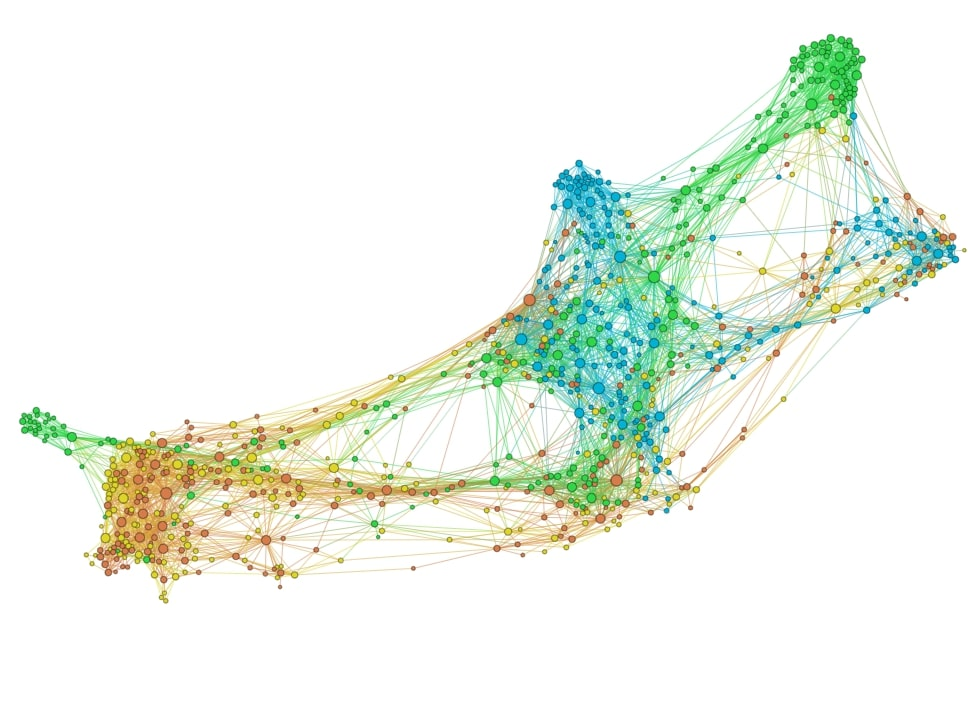
\includegraphics[width=\linewidth, frame]{Graphs/network_vehicle_lrnet.jpg}
    \caption{LRNet}
    \label{fig:wine_lrnet}
\end{subfigure}\hfil
\begin{subfigure}{0.45\textwidth}
    \centering
    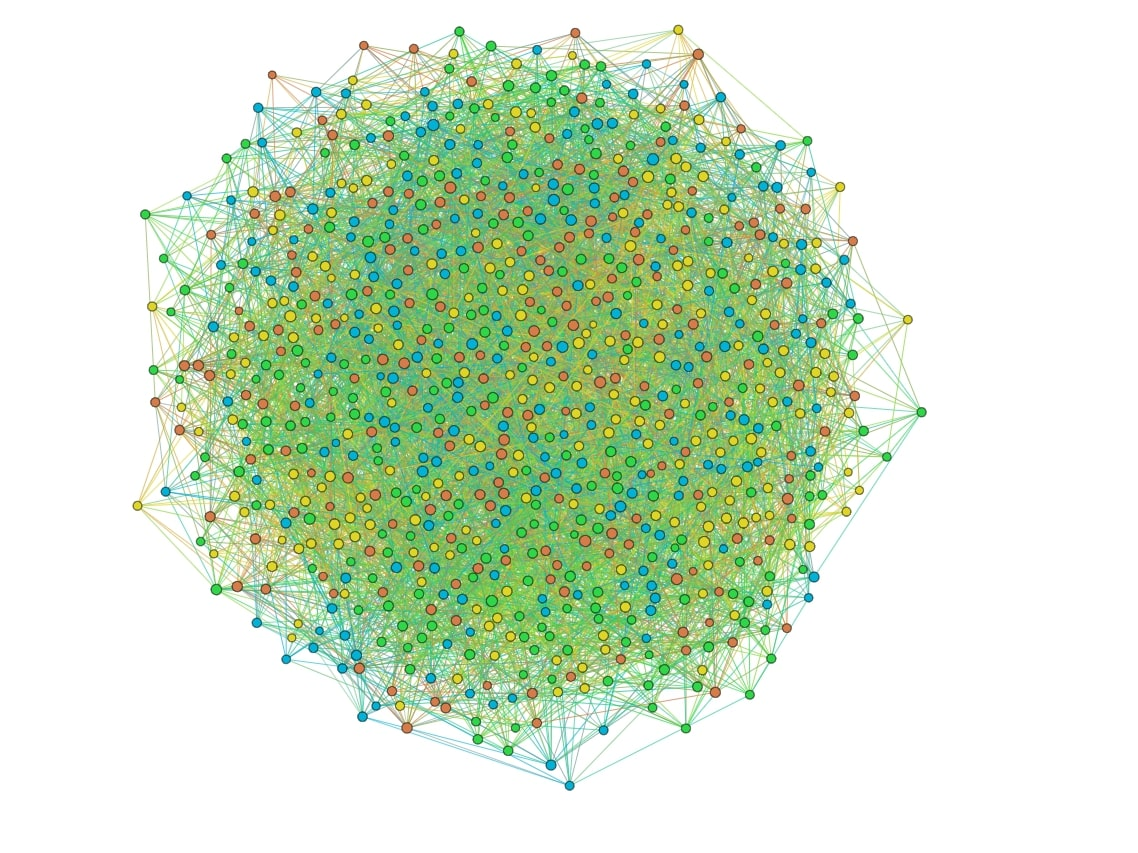
\includegraphics[width=\linewidth, frame]{Graphs/network_vehicle_erdos-renyi.jpg}
    \caption{Erods Renyi}
    \label{fig:wine_erdos_renyi}
\end{subfigure}
\caption{Siete datasetu Vehicle}
\label{fig:wine_networks}
\end{figure}

\subsubsection{Wine dataset}
Dataset Wine obsahuje merania vlastností vína 3 odrôd pestovaných v rovnakej oblasti. 178 meraní je rozdelených do 3 rovnomerne veľkých a dobre oddelených triedy čím sa do veľkej miery podobá datasetu Iris. Hlavný rozdiel je však v počte atribútov ktorých Wine dataset obsahuje 13 vďaka čomu môže priniesť zaujímavé výsledky v porovnaní s datasetom Iris. \cite{wine}
\begin{figure}[H]
\centering
\begin{subfigure}{0.45\textwidth}
    \centering
    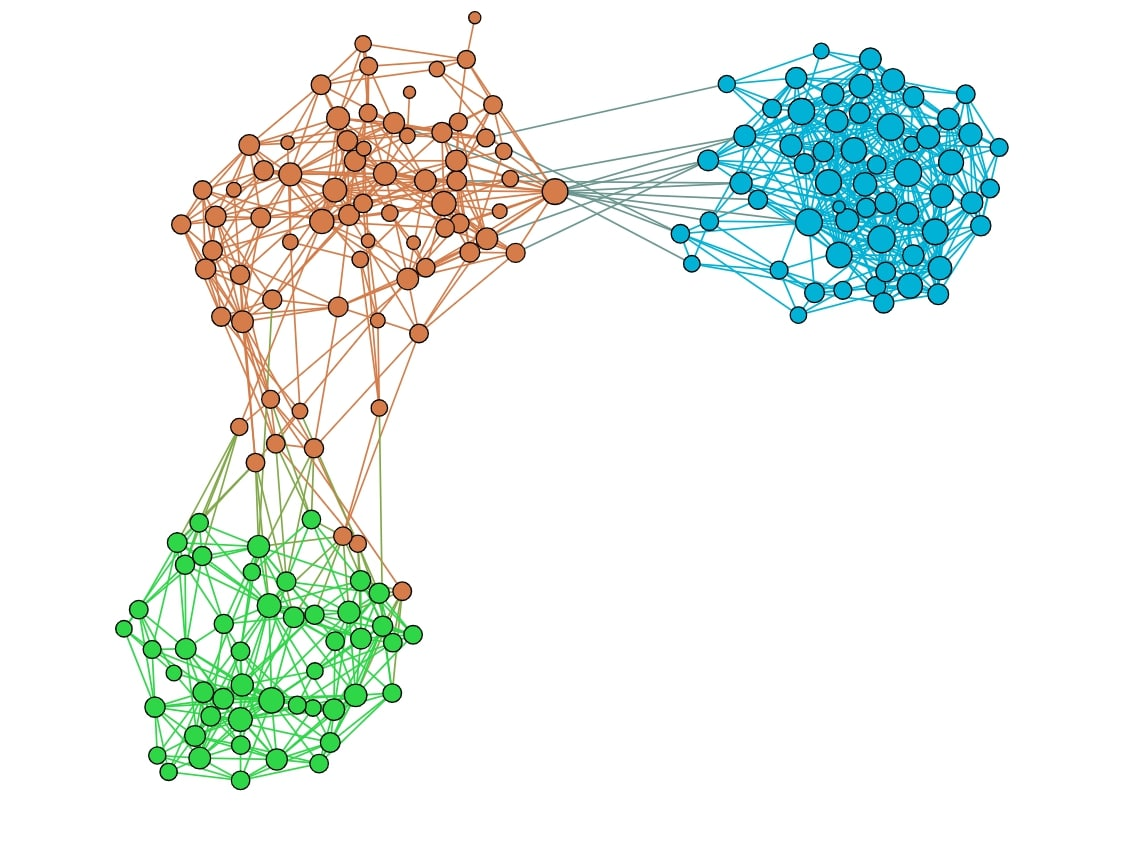
\includegraphics[width=\linewidth, frame]{Graphs/network_wine_knn_epsilon.jpg}
    \caption{kNN + epsilon radius}
    \label{fig:wine_knn_eps}
\end{subfigure}\hfil
\begin{subfigure}{0.45\textwidth}
    \centering
    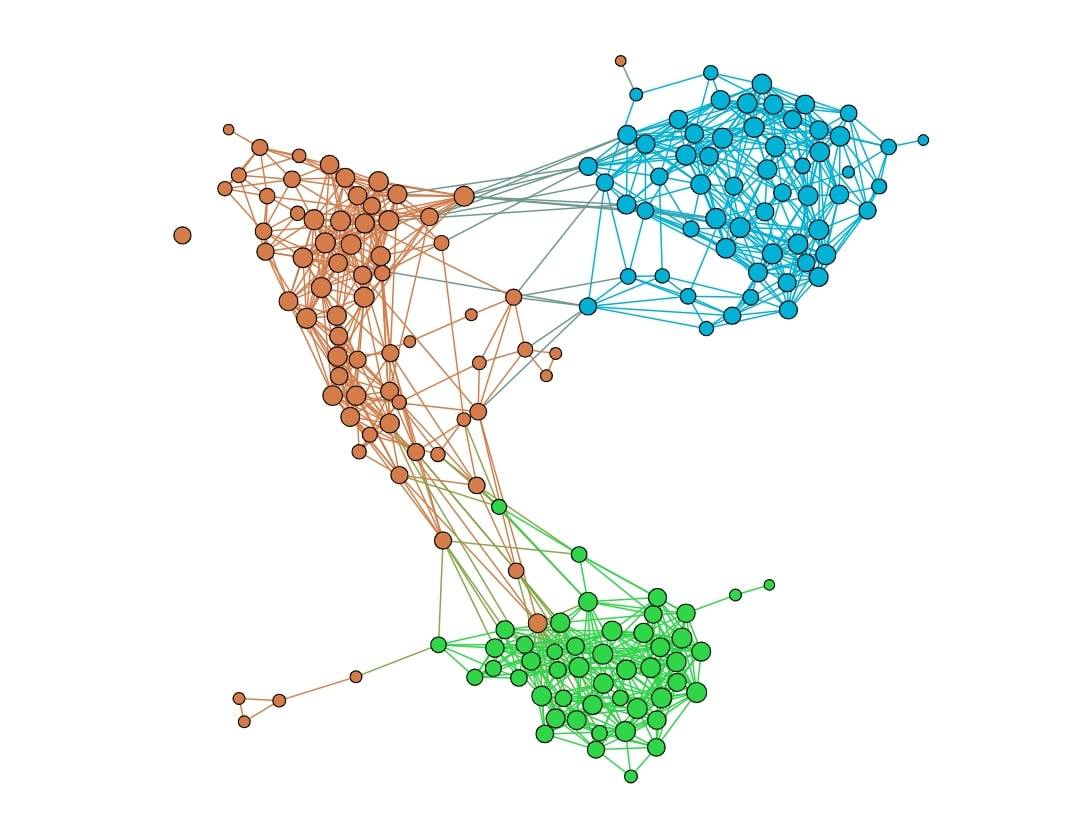
\includegraphics[width=\linewidth, frame]{Graphs/network_wine_nnn.jpg}
    \caption{NNN}
    \label{fig:wine_nnn}
\end{subfigure}
\medskip
\begin{subfigure}{0.45\textwidth}
    \centering
    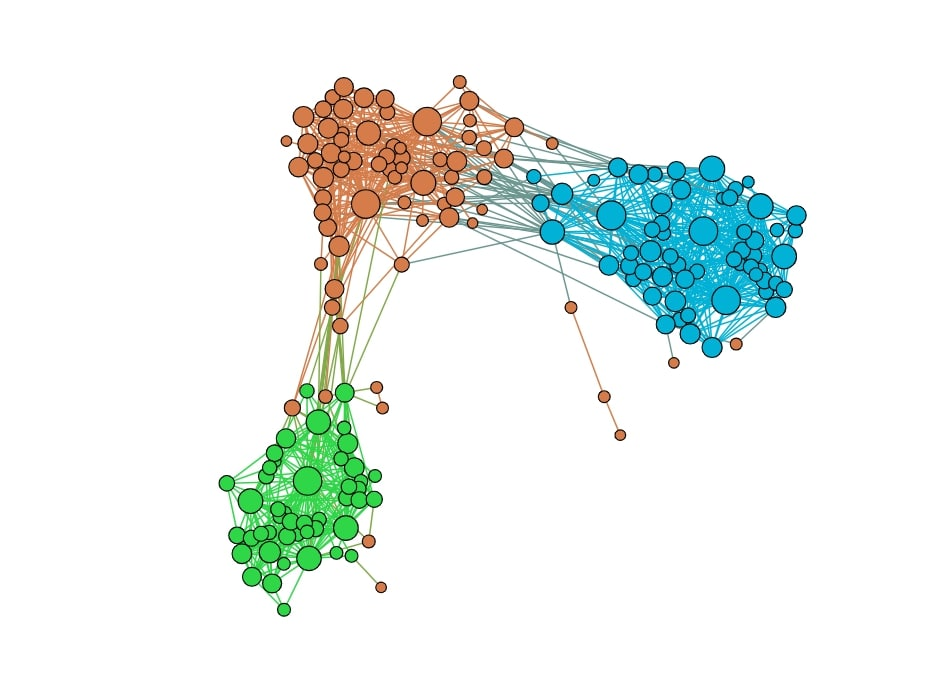
\includegraphics[width=\linewidth, frame]{Graphs/network_wine_lrnet.jpg}
    \caption{LRNet}
    \label{fig:wine_lrnet}
\end{subfigure}\hfil
\begin{subfigure}{0.45\textwidth}
    \centering
    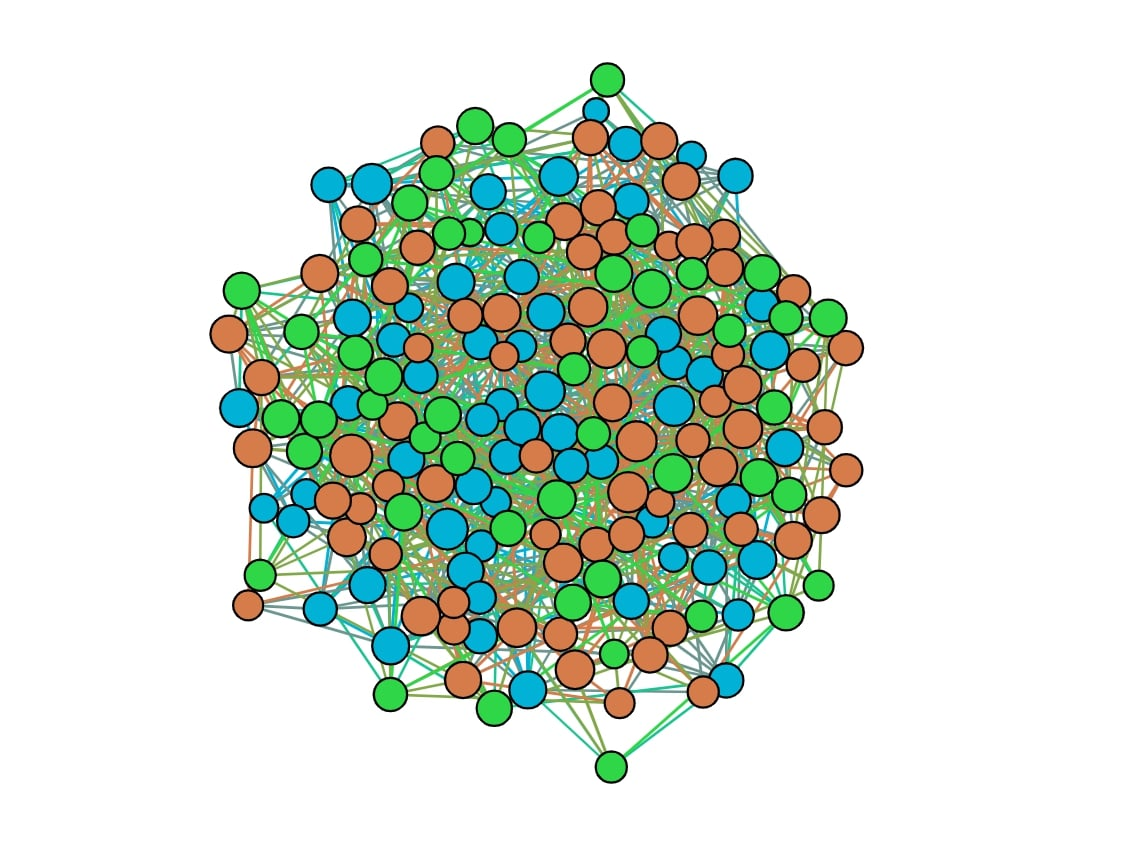
\includegraphics[width=\linewidth, frame]{Graphs/network_wine_erdos_renyi.jpg}
    \caption{Erods Renyi}
    \label{fig:wine_erdos_renyi}
\end{subfigure}
\caption{Siete datasetu Wine}
\label{fig:wine_networks}
\end{figure}

\subsection{Kvalita sieti generovaných jednotlivými
algoritmami}\label{datasets_metrics}

Prvý experiment sa zameriava porovnanie kvality sieti generovaných vyššie uvedenými algoritmami. Pre experimenty bolo zvolených niekoľko typických datasetov pre klasifikáciu uvedených v predchádzajúcej podkapitole \ref{used_dataset}. Pre každý dataset boli vygenerované siete s rovnakou hustotou. Referenčná hustota bola spočítaná na sieti generovanou algoritmom LRNet, ktorý bol použitý so základným nastavením. Pre nastavenie ostatných algoritmov tak, aby mali približné rovnakú hustotu bola využitá aplikácia ktorá je súčasťou tejto práce. Pre každú sieťou bola spočítaná presnosť zaradenia vrcholu do sieťe. Pre tento účel boli použité 2 príbuzné miery uvedené v článku zameranom na algoritmus LRNet. \cite{lrntet}

Prvá miera s názvom \textit{ vážená presnosť zradenia vrcholu (VPZV)} je spočítaná ako priemerná presnosť zaradenia  vrcholov. Presnosť zaradenia vrcholu je určená ako pomer súčtu váh hrán so susediacimi vrcholmi rovnakej triedy $w_{pos}$ a súčtu váh hrán všetkých susedov $w_{all}$. 

\begin{equation}
    w = \frac{w_{pos}}{w_{all}}
\end{equation}

Druhá miera je vypočítaná z predchádzajúcej a bola pomenovaná ako \textit{ nevážená presnosť zaradenia vrcholu (NPZV)}. V tejto miere je presnosť zaradenia vrcholu binárna. Presnosť nadobúda hodnotu $w=1$ v prípade že súčet váh hrán s vrcholmi rovnakej triedy je najväčší, inak nadobúda hodnotu $w=0$. Výsledná presnosť je taktiež určená ako priemer jednotlivých presnosti.

\subsubsection{Výsledky experimentu}

Pre lepšie vyhodnotenie výsledkov oboch metrík je v tejto práci uvedená tabuľka z článku \cite{easeofaccess} kde boli testované rovnaké datasety ako v tejto práci.
\begin{figure}[H]
\centering
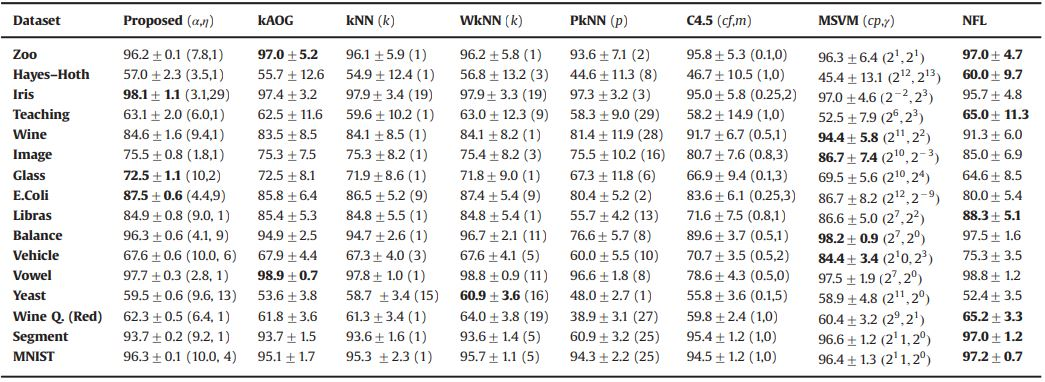
\includegraphics[width=\textwidth]{datasets_ease.JPG}
\caption{Prehľad výsledkov experimentov použitých v článku \cite{easeofaccess} }
\label{datasets_acc}
\end{figure} 


\begin{table}[H]
\centering
\begin{tabular}{|c|c|c|c|c|}
\hline
\textbf{Algoritmus} & \textbf{Parametre algoritmu} & \textbf{\begin{tabular}[c]{@{}c@{}}vážená\\ presnosť\end{tabular}} & \textbf{\begin{tabular}[c]{@{}c@{}}nevážená\\ presnosť\end{tabular}} & \textbf{\begin{tabular}[c]{@{}c@{}}hustota\\ siete\end{tabular}} \\ \hline
Knn + epslion       & k=9, eps=0.999               & \textbf{95.3 }                                                                         & \textbf{96.0}                                                                             & 0.063                                                            \\ \hline
NNN                 & n=13                         & 93.3                                                                          & 94.7                                                                            & 0.062                                                            \\ \hline
Lrnet               & minVertex =1, reduction =1   & 91.0                                                                           & 95.3                                                                            & 0.063                                                            \\ \hline
ErdosRenyi          & p=0.0315                     & 49.8                                                                          & 54.7                                                                            & 0.063                                                            \\ \hline
\end{tabular}
\caption{Vlastnosti sieti pre Iris dataset}
\end{table}



\begin{table}[H]
\centering
\begin{tabular}{|c|c|c|c|c|}
\hline
\textbf{Algoritmus}                                       & \textbf{Parametre algoritmu} & \textbf{\begin{tabular}[c]{@{}c@{}}vážená\\ presnosť\end{tabular}} & \textbf{\begin{tabular}[c]{@{}c@{}}nevážená\\ presnosť\end{tabular}} & \textbf{\begin{tabular}[c]{@{}c@{}}hustota\\ siete\end{tabular}} \\ \hline
\begin{tabular}[c]{@{}c@{}}Knn +\\   epslion\end{tabular} & k=5, eps=0.9843              & 86.3                                                                          & \textbf{79.9 }                                                                           & 0.38                                                             \\ \hline
NNN                                                       & n=19                         & \textbf{87.2 }                                                                         & 79.8                                                                            & 0.37                                                             \\ \hline
Lrnet                                                     & minVertex =1, reduction =1   & 85.4                                                                          & 77.7                                                                            & 0.38                                                             \\ \hline
ErdosRenyi                                                & p=0.018                      & 42.3                                                                          & 40.3                                                                            & 0.38                                                             \\ \hline
\end{tabular}
\caption{Vlastnosti sieti pre E.Coli dataset}
\end{table}



\begin{table}[H]
\centering
\begin{tabular}{|c|c|c|c|c|}
\hline
\textbf{Algoritmus}                                       & \textbf{Parametre algoritmu} & \textbf{\begin{tabular}[c]{@{}c@{}}vážená\\ presnosť\end{tabular}} & \textbf{\begin{tabular}[c]{@{}c@{}}nevážená\\ presnosť\end{tabular}} & \textbf{\begin{tabular}[c]{@{}c@{}}hustota\\ siete\end{tabular}} \\ \hline
\begin{tabular}[c]{@{}c@{}}Knn +\\   epslion\end{tabular} & k=10, eps=0.9965             & 61.6                                                                          & 64.5                                                                            & 0.05                                                             \\ \hline
NNN                                                       & n=17                         &\textbf{ 63.1  }                                                                        &\textbf{ 68.2   }                                                                         & 0.048                                                            \\ \hline
Lrnet                                                     & minVertex =1, reduction =1   & 60.9                                                                          & 63.6                                                                            & 0.05                                                             \\ \hline
ErdosRenyi                                                & p=0.0245                     & 36.9                                                                          & 36.4                                                                            & 0.05                                                              \\ \hline
\end{tabular}
\caption{Vlastnosti sieti pre Glass dataset}
\end{table}


\begin{table}[H]
\centering
\begin{tabular}{|c|c|c|c|c|}
\hline
\textbf{Algoritmus}                                       & \textbf{Parametre algoritmu} & \textbf{\begin{tabular}[c]{@{}c@{}}vážená\\  presnosť\end{tabular}} & \textbf{\begin{tabular}[c]{@{}c@{}}nevážená\\  presnosť\end{tabular}} & \textbf{\begin{tabular}[c]{@{}c@{}}hustota\\ siete\end{tabular}} \\ \hline
\begin{tabular}[c]{@{}c@{}}Knn +\\   epslion\end{tabular} & k=50, eps=0.99               & \textbf{51.9}                                                                          & 57.0                                                                             & 0.032                                                            \\ \hline
NNN                                                       & n=85                         & 51.8                                                                          &\textbf{ 58.2}                                                                              & 0.032                                                            \\ \hline
Lrnet                                                     & minVertex =1, reduction =1   & 51.2                                                                          & 57.0                                                                             & 0.032                                                            \\ \hline
ErdosRenyi                                                & p=0.0245                     & 44.9                                                                          & 45.2                                                                            & 0.032                                                            \\ \hline   
\end{tabular}
\caption{Vlastnosti sieti pre Wine red dataset}
\end{table}

\begin{table}[H]
\centering
\begin{tabular}{|c|c|c|c|c|}
\hline
\textbf{Algoritmus} &
  \textbf{\begin{tabular}[c]{@{}c@{}}Parametre\\  algoritmu\end{tabular}} &
  \textbf{\begin{tabular}[c]{@{}c@{}}vážená\\  presnosť\end{tabular}} &
  \textbf{\begin{tabular}[c]{@{}c@{}}nevážená\\  presnosť\end{tabular}} &
  \begin{tabular}[c]{@{}c@{}}hustota \\ siete\end{tabular} \\ \hline
\textbf{\begin{tabular}[c]{@{}c@{}}Knn +\\  epslion\end{tabular}} & k=10, eps=0.999            &\textbf{ 94.1} & \textbf{97.8} & 0.061 \\ \hline
\textbf{NNN}                                                      & n=17                       & 92.9 & 96.1 & 0.062 \\ \hline
\textbf{Lrnet}                                                    & minVertex =1, reduction =1 & 90.5 & 95.5 & 0.062 \\ \hline
\textbf{ErdosRenyi}                                               & p=0.031                    & 52.8 & 61.2 & 0.059 \\ \hline
\end{tabular}
\caption{Vlastnosti sieti pre Wine  dataset}
\label{tab:wine_quality_dnesity}
\end{table}

\begin{table}[H]
\centering
\begin{tabular}{|c|c|c|c|c|}
\hline
\textbf{Algoritmus} &
  \textbf{\begin{tabular}[c]{@{}c@{}}Parametre\\  algoritmu\end{tabular}} &
  \textbf{\begin{tabular}[c]{@{}c@{}}vážená\\  presnosť\end{tabular}} &
  \textbf{\begin{tabular}[c]{@{}c@{}}nevážená\\  presnosť\end{tabular}} &
  \begin{tabular}[c]{@{}c@{}}hustota \\ siete\end{tabular} \\ \hline
\textbf{\begin{tabular}[c]{@{}c@{}}kNN +\\ epslion\end{tabular}} & k=24, eps=0.99             & 62.9 &\textbf{ 69.1} & 0.028 \\ \hline
\textbf{NNN}                                                      & n=33                       &\textbf{ 63.5} & 70.2 & 0.028 \\ \hline
\textbf{Lrnet}                                                    & minVertex =1, reduction =1 & 58.4 & 64.1 & 0.028 \\ \hline
\textbf{ErdosRenyi}                                               & p=0.014                    & 42.7 & 30.3 & 0.027 \\ \hline
\end{tabular}
\caption{Vlastnosti sieti pre Vehicle dataset}
\label{tab:vehicle_dnesity}
\end{table}

\subsubsection{Zhodnotenie experimentu}
Z výsledkov experimentu môžeme usúdiť že presnosť oboch metrík, váženej presnosť zaradenia vrcholu a neváženej presnosti zaradenia vrcholy, sa pohybuje v rozsahu presností klasifikačných algoritmov uvedených v tabuľke \ref{datasets_acc}. Taktiež môžme pozorovať že siete generované rôznymi algoritmami majú podobnú presnosť zaradenia vrcholov. 

Výsledná presnosť poskytuje intuíciu že algoritmy určené pre prevod vektorových dát na sieť zachovávajú požadovane vlastnosti dát. Výnimku tvorí sieť generovaná algoritmom \textit{Erdos Renyi}. Tento algoritmus však nie je určený pre prevod vektorových dát na sieť čim upevňuje intuíciu o potrebe špecializovaných algoritmov. 

Autor metrík neposkytuje ďalšie informácie o fungovaní vyššie uvedených metrík ale vzhľadom na ich nízku výpočetnu náročnosť oproti klasickým klasifikačným algoritmom predstavujú priestor pre skúmanie. Na základe týchto výsledkov boli vykonané dva experimenty. Prvý experiment môžeme zaradiť k exploatačnej analýze siete a bližšie skúma vplyv hustoty na presnosť zaradenia.  Ďalšie experimenty sa zameriavajú na vplyv na rôzne faktory ovplyvňujúce presnosť klasifikácie.

\subsection{Vplyv hustoty siete na presnosť zaradenia vrcholu}
\label{exp:density_impact}
Ako bolo naznačené v predchádzajúcom experimente, cieľom tohoto experimentu je vytvoriť náhľad na to ako vplyva hustota siete na výsledky presnosti zaradenia vrcholov vypočítane pomocou vyššie uvedených metrík. 

\subsubsection{Príprava experimentu}
Keďže aplikácia ani knižnice vytvorené v tejto prací neodhalili potrebu podobného využitá boli najskôr implementované potrebne súčasti nutné pre tento experiment.  Vzhľadom k tomu že potreba tejto funkcionality bola odhalená až vo fáze vykonávania experimentov, boli vytvorené len triedy pre vyhodnocovanie kvality sieti pre rôzne nastavenia parametrov. Výsledky experimentov boli uložené do súborov vo formáte \textit{.json} a pre vizualizáciu bola vytvorená statická webová stránka ktorá súbory načíta z lokálneho úložiska a zobrazuje vo forme grafov. Detailnejší popis tried vytvorených pre tento experiment je popísaný v kapitole \ref{cap:network_construction}.

\subsubsection{Nastavenie parametrov}
Pre všetky datasety použité v tejto práci boli použité rovnaké nastavenia konkrétnych algoritmov. Algoritmy LRnet a kNN + $\epsilon-radius$ majú dva konfigurovateľné parametre ktoré do veľkej miery ovplyvňujú výslednú sieť. Hľadanie ideálnej kombinácie týchto parametrov je cieľom viacúčelovej optimalizácie ktorá presahuje zameranie tejto práce a preto boli použite algoritmy založené na náhodnom prehľadávaní okolia.

Je nutné podotknúť že pri algoritme kNN + $\epsilon-radius$  náhodná voľba medzí zmenou parametru \textit{k} alebo parametru $\epsilon$  môže spôsobovať väčšie nepresnosti. Tento problém je umocnený faktom že algoritmus bol adaptovaný na použite podobnosti, ktoré je odlišné od typickej implementácii ktoré využívajú vzdialenosť, a je citlivejšie na nastavenie parametrov. Použite podobnosti ovplyvňuje predovšetkým časť v ktorej použité  $\epsilon$ okolie, čiže časť kde je vrchol spojený so všetkými susedami v $\epsilon $ okolí. Použitie $\epsilon$ okolia  môže spôsobiť že malá zmena parametru $\epsilon$ môže viesť k veľkému rozdielu v množstve použitých vrcholov čo pri použití s podobnosťou \textit{gaussian kernel} môže viesť k skresleným výsledkom. Nesprávne nastavenie však nespôsobí úplne zlyhanie algoritmu ale v najhoršom prípade algoritmus zdegraduje na izolovaný kNN alebo $\epsilon - radius$.

Pri algoritme LRNet nastáva podobný problém. Algoritmus LRnet sa však funguje na princípe že základne nastavenie algoritmu poskytuje dobré výsledky a zlepšenie, respektíve zhoršenie môže byť dosiahnuté pomocou lokálneho prehľadávania v okolí základného nastavenia čo prináša značnú výhodu oproti algoritmu kNN + $\epsilon-radius$.

Nastavenie parametrov experimentu pre rôzne algoritmy:
\begin{itemize}
\item kNN + $\epsilon-radius$:
\begin{itemize}
    \item \textbf{k}= 1
    \item\textbf{krok k} = +2
    \item\textbf{max k} = veľkosť najväčšej triedy
    \item \textbf{epsilon} = 1.0
    \item \textbf{krok epsilon} = - 0.005 
\end{itemize}
\item LrNet
\begin{itemize}
    \item \textbf{min deegres} =1
    \item\textbf{krok min deegres} = +2
    \item \textbf{max min deegres} = veľkosť najväčšej triedy
    \item \textbf{reduction ratio} = 0.1
    \item\textbf{krok reduction ratio} = + 0.1
\end{itemize}
\item NNN
\begin{itemize}
    \item\textbf{n} = 1
    \item \textbf{krok n} = +2
    \item \textbf{max n} = veľkosť najväčšej triedy
\end{itemize}
\item Erdos Renyi
\begin{itemize}
    \item \textbf{p} = 0.005
    \item\textbf{ krok p} = 0.005
    \item\textbf{ max p} = 1
\end{itemize}
\end{itemize}

Okrem nastavenia parametrov špecifických pre algoritmy bol nastavený parameter predčasného ukončenia ak hustota siete dosiahne 50\%.


\subsubsection{Výsledky a zhodnotenie experimentu}
Pre ilustráciu výsledkov bol zvolený dataset \textit{Vehcile} a dataset \textit{E.Coli}. Výsledky pre ostatné datasety sú umiestnene v prílohe. 

\begin{figure}[H]
\label{plot_ecoli_base}
\centering
    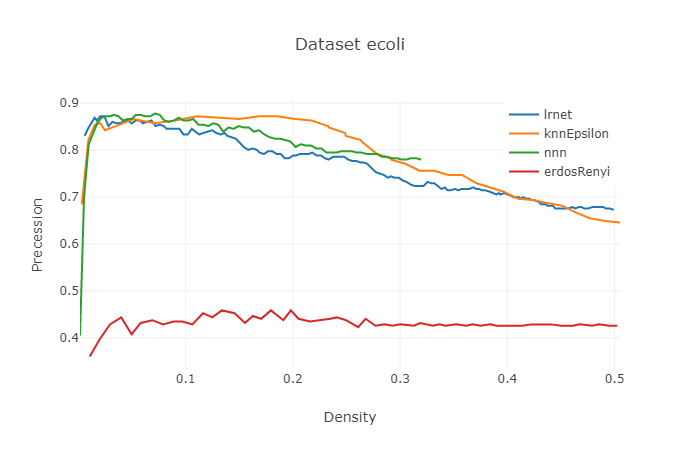
\includegraphics[width=\textwidth]{Plots/plot_ecoli_base.png}
    \caption{Vplyv hustoty siete na kvalitu zaradenia pre dataset Ecoli}
\end{figure} 

\begin{figure}[H]
\centering
    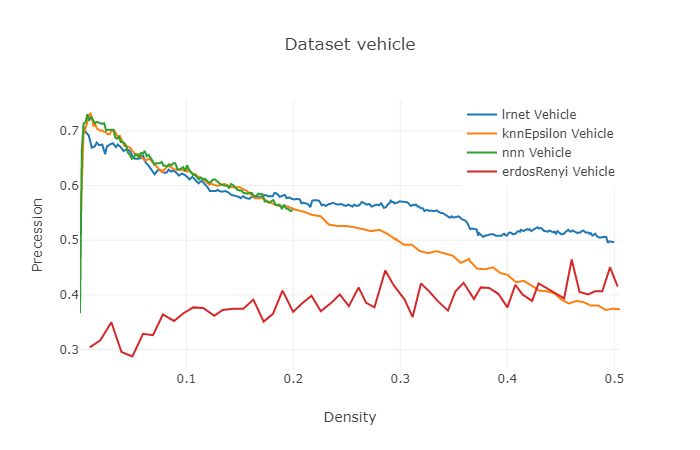
\includegraphics[width=\textwidth]{Plots/plot_vehicle_base.png}
    \caption{Vplyv hustoty siete na kvalitu zaradenia pre dataset Vehicle}
\end{figure} 

Z výsledkov experimentov môžeme usúdiť že kvalita zaradenia vrcholov klesá s hustotou. Výnimku tvoria dataset Iris a Wine ktoré tvoria veľmi dobré oddelené zhluky.Vďaka dobrej oddelenosti sú pri týchto datasetov vrcholy dobré zradené aj pri relatívne vysokej hustote. Pri niektorých datasetoch môžeme vidieť že výsledne siete vytvorené algoritmom kNN + $\epsilon-radius$ sú značne odlišné. Táto odlišnosť je najviac viditeľná pre dataset E.Coli a preto bol vykonaný experiment ktorý sa zameriava na skúmanie tohto výsledku. Z výsledkov vo forme grafov môžme vidieť že vrcholy sú najlepšie zradené pri veľmi nízkych hustotách grafoch. Tento výsledok je spôsobený že pri nízkej hustote je sieť zvyčajne tvorená jednou veľkou komponentov a množstvom malých, často jednoprvkových komponent. Izolované, respektíve veľmi mále komponenty sú pri \textbf{klasifikácii} nežiadané a preto je nutné overiť množstvo a veľkosť komponent a brať do úvahy len siete ktoré majú nízky počet malých komponent.  

\subsection{Detailný pohľad na algoritmus $ kNN + \epsilon-radius$}
Predchádzajúci experiment okrem iného odhalil odchýlky algoritmu kNN + $\epsilon-radius$ od výsledkov ostatných algoritmov. Toto správanie je najlepšie rozoznateľne z výsledkov prechádzajúceho experimentu pre dataset E.coli \ref{plot_ecoli_base}. Interval kde tento algoritmus vytvára siete s lepším zaradením vrcholov síce neobsahuje najlepší výsledok ale aj tak predstavuje zaujímavú oblasť pre preskúmanie. Cieľom tohto experimentu je zistiť čo spôsobuje dané výsledky.

\subsubsection{Nastavenie experimentu}
Ako prvý krok experimentu bol algoritmus spustený s použitím jedeného parameteru pričom druhý parameter bol nastavený tak aby nebol pri vytváraní sieti použitý. V ďalšom kroku bolo zvolených niekoľko nastavení kde izolované algoritmy poskytovali najlepšie výsledky následne boli algoritmus spustený s zafixovaným nastavením jedeného parametru.

\subsubsection{Výsledky experimentu}

\begin{figure}[H]
\centering
    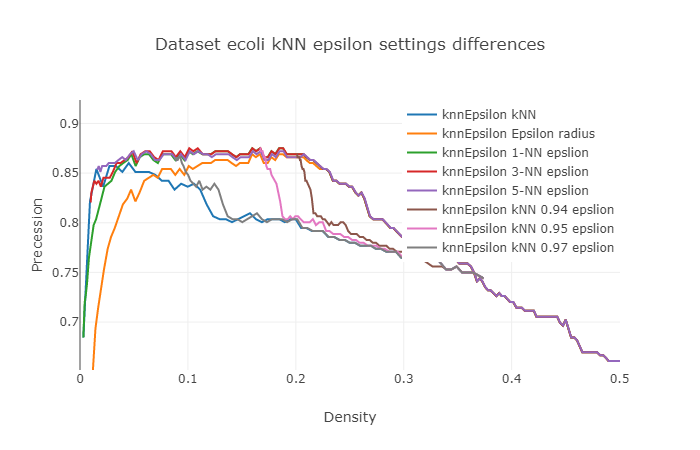
\includegraphics[width=\textwidth]{Plots/plot_knn_epsilon_ecoli.png}
    \caption{Presnosť zaradenia vrcholov pre rôzne nastavenia algoritmu kNN + $\epsilon-radius$}
    \label{plot_ecoli_base}
\end{figure} 
Legenda na obrázku \ref{plot_ecoli_base} naznačuje ktorý parameter bol zafixovaný a s akým nastavením parametru. V prípade prvých dvoch meraní bol jeden z parametrov nastavený tak aby sa pri vytváraní sieťke neprejavil a hybridný algoritmus bol redukovaný na jeden z dvoch jednoduchších algoritmov.
\subsubsection{Zhodnotenie Experimentu}
Výsledky experimentu ukázali že odchýlka na obrázku \ref{plot_ecoli_base} nebola spôsobená náhodou ale vďaka dobrým výsledkom časti algoritmu kde je aplikovaný $\epsilon$ rádius. Ďalej môžeme pozorovať že pri malých zmenách jedného alebo druhého parametru algoritmus rýchlo konverguje ku kNN alebo k $\epsilon$ rádius. Pri detailnejšom pohľade na výsledky na obrázku \ref{ecoli_knn_epsilon_best} môžme ďalej konštatovať že použite hybridného algoritmu videlo k zlepšeniu najlepšieho výsledku pre algoritmus epsilon o 1\% a taktiež môžeme pozorovať že použitie hybridného algoritmu videlo k výraznému zlepšeniu pre riedke siete. Zo siete na obrázku \ref{ecoli_knn_epsilon_best}  môžeme ďalej usúdiť že v prípade malej zmeny parametrov budu hraný vytvárane prioritne medzi vrcholmi dobre oddelených komponent čo spôsobuje relatívne dlhý interval na ktorom je tento výsledok stabilný.

\begin{figure}[H]
\centering
\begin{subfigure}{0.45\textwidth}
    \centering
    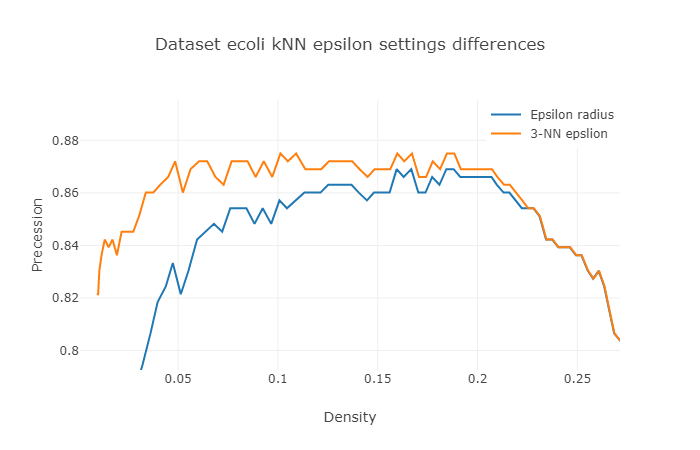
\includegraphics[width=\linewidth]{Plots/plot_ecoli_knn_epsilon_best.png}
    \caption{Porovnanie najlepšieho výsledku algoritmov epsilon rádius a kNN + $\epsilon-radius$}
\end{subfigure}
\begin{subfigure}{0.45\textwidth}
    \centering
    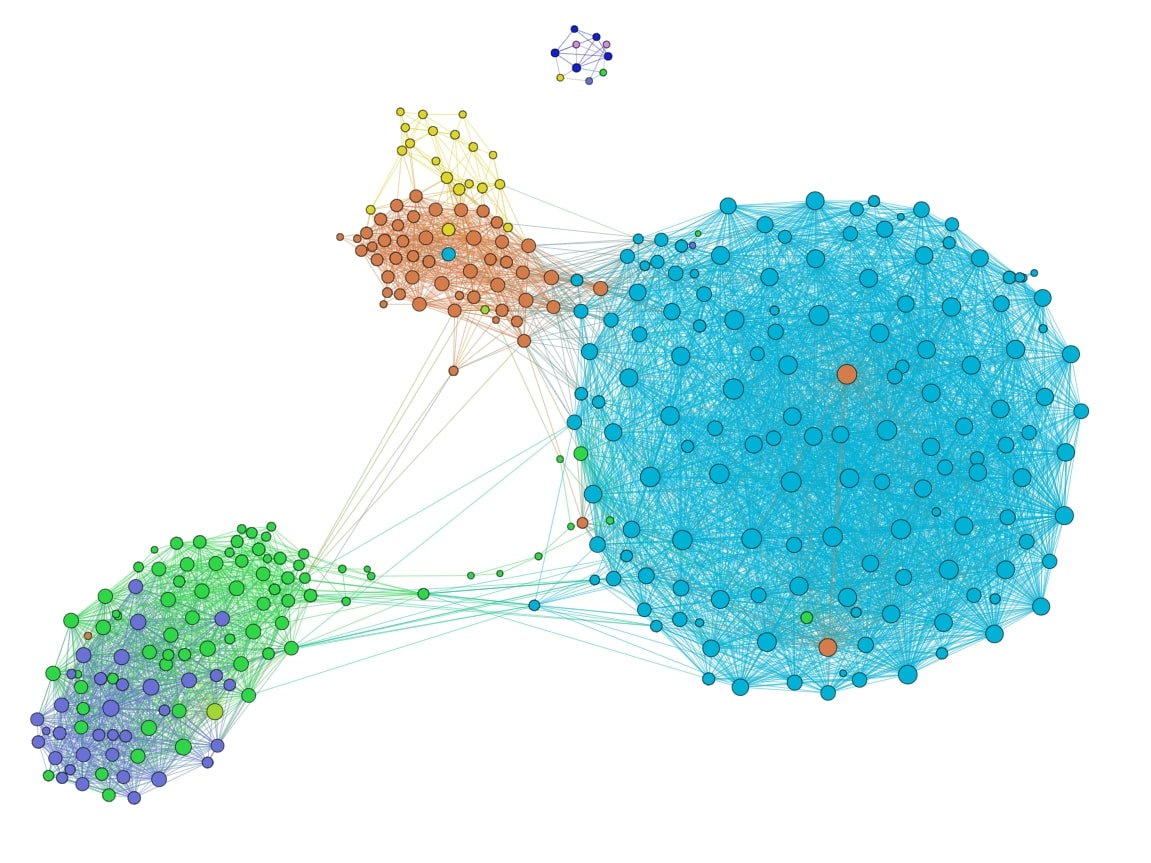
\includegraphics[width=\linewidth]{Graphs/network_ecoli_knn_epsilon_best.jpg}
    \caption{Sieť (najredšia) pre najlepší výsledok zaradenia vrcholov}
\end{subfigure}\hfil
\caption{Najlepšia presnosť zaradenia vrcholov E.Coli datasetu pre algoritmus kNN + $\epsilon-radius$}
\label{ecoli_knn_epsilon_best}
\end{figure}


\subsection{Porovnanie algoritmov pre klasifikáciu pomocou siete}
V predchádzajúcich experimentov bola venovaná pozornosť predovšetkým skúmaniu sieti vytvorených jednotlivými algoritmami. Výsledky ukázali že siete s neúzkou hustotou zvyčajne poskytujú lepšie výsledky zaradenia vrcholov do siete.

Tento experiment sa zameriava na porovnanie výsledkov klasifikačných algoritmov \textit{ease of access} a \textit{average link weigth}. Najľahší spôsob určenia presnosti klasifikácie predstavuje takzvané mriežkové hľadanie. Tento spôsob je však výpočtovo veľmi náročný a v kombinácii s nastaveniami algoritmov pre konštrukciu sieti predstavuje veľmi neafektívne riešenie. Pri klasifikácii pomocou sieti je najdôležitejším parameterom počet vrcholov ktoré budu použité pri klasifikácii. Tento počet závisí od množstva parametrov ale predovšetkým od samotnej siete. Z tohoto dôvodu je vhodné použiť počet vrcholov na základe vlastnosti ktorá sa dá spočítať priamo zo siete použitej pre klasifikáciu. V tomto experiment je zvolenou vlastnosťou priemerný stupeň.

\subsubsection{Príprava tréningovej siete}
Pre porovnanie presnosti algoritmov bola zvolená 10-násobná kros-validácia. Dataset bol náhodne rozdelený do 10 skupín s rovnomerným zastúpením tried a postupne bola zvolená každá skupina ako testovacia sada a z ostatných 9 skupín bola vytvorená tréningová sieť pomocou zvoleného algoritmu. Daný postup bol zopakovaný pre oba algoritmy 50 krát pre vylúčenie odchýlky merania.

\subsubsection{Nastavenie parametrov}
Nastavenie parametrov môžeme rozdeliť do 3 krokov.
\begin{enumerate}
\item \textbf{nastavenie podobnosti} - ovplyvňuje generovanú maticu podobnosti. Pre tento experiment bola zvolená podobnosť \textit{gaussian kernel} a dáta boli normalizované a reškalované do intervalu $<0,1>$
\item \textbf{nastavenie konštrukcie siete} - parametre použitých algoritmov boli nastavené tak, aby generovali sieť s rovnakou hustotou. Pre tento experiment boli využité nastavenia z kapitoly \ref{datasets_metrics}.

\item \textbf{nastavenie klasifikácie} - ako bolo naznačené, pre určenie presnosti klasifikácie bola použitá k-násobná kros-validácia s parametrom $k=10$ a samotný výsledok bol určený ako priemer 50 opakovaní klasifikácie s náhodne generovanými rozdeleniami tréningových a testovacích objektov. \\ Pre algoritmus \textit{Average Link Weigth} je bezparametrický čiže ďalšie nastavenie nebolo potrebné. Algoritmus \textit{Ease of Access} ma 3 parametre. Pre pramater epsilon bola zvolená hodnota 10, pri ktorej boli experimentálne zistené \cite{easeofaccess} stabilne dobré výsledky pre rôzne datasety. Parameter pre nastavenie počtu iterácii markovho reťazca bol nastavený na hodnotu 10, pričom bol použitá implementácia ktorá ukončuje markov reťazec predčasne ak sa vektor s pravdepodobnosťami od poslednej iterácie nezmení.  Posledný parameter určuje koľko susedov vrchola sa má použiť pre samotnú klasifikáciu. Tento parameter bol nastavený na priemerný stupeň siete, rovnako ako pre algoritmus \textit{Average Link Weigth}.
\end{enumerate}

\subsubsection{Výsledky experimentu}

\begin{table}[H]
\centering
\begin{tabular}{|c|c|c|c|c|c|c|}
\hline
\textbf{}              &\textbf{Iris}                                   &\textbf{E.coli}                                    &\textbf{Glass}                                 &\textbf{Wine red}                              & \textbf{Vehicle}                          & \textbf{Wine} \\ \hline
\textbf{kNN + epislon} &\makecell{95.4 \\ \pm 0.002}                    &\makecell{86.2 \\ \pm 0.002}                       &\makecell{62.9 \\ \pm 0.004}                   &\makecell{57.7  \\ \pm 0.002}                  &\makecell{68.3  \\ \pm 0.004}              &\makecell{96.1 \\ \pm 0.002} \\ \hline   
\textbf{NNN}           &\makecell{95.2 \\ \pm 0.001}                    &\makecell{85.9 \\ \pm 0.002}                       &\makecell{64.2 \\ \pm 0.005}                   &\makecell{58.0 \\ \pm 0.002}                   &\makecell{68.5  \\ \pm 0.005}              &\makecell{\textbf{96.8} \\ \pm \textbf{0.002}}                    \\ \hline
\textbf{LRNet}         &\makecell{\textbf{96.1} \\ \pm \textbf{0.002}}  &\makecell{86.5 \\ \pm 0.002}                       &\makecell{60.2 \\ \pm 0.006}                   &\makecell{57.4 \\ \pm 0.002}                   &\makecell{68.4  \\ \pm 0.006}              &\makecell{95.7 \\ \pm 0.002} \\ \hline
\textbf{ErdosRenyi}    &\makecell{95.8 \\ \pm 0.002}                    &\makecell{\textbf{86.6}   \\ \pm \textbf{0.002}}   &\makecell{\textbf{64.4} \\ \pm \textbf{0.006}} &\makecell{\textbf{58.4} \\ \pm \textbf{0.003}} &\makecell{\textbf{68.6}   \\ \pm \textbf{0.004}}  &\makecell{96.4 \\ \pm 0.002} \\ \hline
\end{tabular}
\caption{Presnosť klasifikácie algoritmu Ease of access}
\label{classification_result_mean_EOA}
\end{table}

\begin{table}[H]
\centering
\begin{tabular}{|c|c|c|c|c|c|c|}
\hline
\textbf{}               & \textbf{Iris}                                  & \textbf{E.coli}                              & \textbf{Glass}                                & \textbf{Wine red}                             & \textbf{Vehicle}                                  & \textbf{Wine} \\ \hline
\textbf{kNN + epislon}  &\makecell{ \textbf{95.6} \\ \pm \textbf{0.001}} &\makecell{86.8 \\ \pm 0.002}                  &\makecell{63.8 \\ \pm 0.005}                   &\makecell{57.9 \\ \pm 0.002}                   &\makecell{68.5 \\ \pm 0.003}                       &\makecell{\textbf{ 96.7} \\ \pm \textbf{0.002}}  \\ \hline
\textbf{NNN}            &\makecell{95.4 \\ \pm 0.002}                    &\makecell{\textbf{87.0} \\ \pm \textbf{0.002}}&\makecell{64.1 \\ \pm 0.004}                   &\makecell{\textbf{58.2} \\ \pm \textbf{0.002}} &\makecell{68.4  \\ \pm 0.004}                      &\makecell{96.5 \\ \pm 0.002}           \\ \hline
\textbf{LRNet}          &\makecell{95.2 \\ \pm 0.003}                    &\makecell{86.9 \\ \pm 0.002}                  &\makecell{\textbf{64.2} \\ \pm \textbf{0.005}} &\makecell{\textbf{58.2} \\ \pm \textbf{0.002}} &\makecell{\textbf{68.6} \\ \pm \textbf{0.004}} &\makecell{96.4 \\ \pm 0.003}           \\ \hline
\textbf{ErdosRenyi}     &\makecell{95.2 \\ \pm 0.002}                    &\makecell{86.7 \\ \pm 0.002}                  &\makecell{64.1 \\ \pm 0.005}                   &\makecell{58.1 \\ \pm 0.004}             &\makecell{68.4 \\ \pm 0.003}                       &\makecell{96.6 \\ \pm 0.003}           \\ \hline
\end{tabular}
\caption{Presnosť klasifikácie algoritmu Average link weight}
\label{classification_result_mean_ALW}
\end{table}
Okrem výsledkov klasifikácie uvedených v tabuľkách \ref{classification_result_mean_EOA} a \ref{classification_result_mean_ALW} bola vypočítané aj konfidenčne intervaly. Výsledok ukázal že pre väčšinu sieti sa 95\% konfidenčne interval pohyboval medzi +- 0.001 a +- 0.003 bez ohľadu na použité algoritmy pre zostrojenie siete a klasifikáciu. Výnimku tvorí iba dataset Glass u ktorého sa 95\% konfidenčný interval pohybuje medzi +- 0.004 a +- 0.007. Výsledky ukazujú veľmi dobrú stabilitu oboch klasifikačných algoritmov. Rozdiel medzi datasetom Glass a ostatnými datasetmi je zanedbateľný a preto nebude ďalej skúmaný.

\subsubsection{Zhodnotenie experimentu}
Výsledky experimentu na prvý pohľad naznačujú, že siete s rovnakou hustotou ktoré boli zostrojené rôznymi algoritmami poskytujú rovnako dobré výsledky klasifikácie. Zaujímavý je aj výsledok klasifikácie pomocou siete zostrojenej technikou \textit{Erdos Renyi}, kde je výsledok klasifikácie rovnaký ako pri použití špecializovaných algoritmov.

Po hlbšom skúmaní výsledku tohoto experimentu boli určené dve hlavné príčiny. Hlavnou príčinou bolo vytvorenie sieti  s rovnakou hustotou v kombinácii s použitím priemerného stupňa siete pri samotnej klasifikácii. Keďže siete s  rovnakou hustotou majú aj rovnaký priemerný stupeň, výber vrcholov použitých pri klasifikácie je podobný.

Vzhľadom k vyššie uvedeným zaisteniam bol experiment zopakovaný znova pričom bola použitá odlišná stratégia pre voľbu počtu vrcholov.

\subsection{Vplyv počtu vrcholov na výsledok klasifikácie}
Z výsledku prechádzajúceho experimentu vyplynulo že ak pri sú pre klasifikáciu použite siete s rovnakou hustotou a ak je použitý priemerný stupeň pri samotnej klasifikácie, sieť samotná nemá na klasifikáciu vplyv.

Tento experiment sa zameriava na sledovanie vplyvu počtu vrcholov na výsledok klasifikácie. V predchádzajúcom experimente bolo okrem samotného výsledku zistené že pri voľbe počtu vrcholov je priemerný stupeň nevhodný a špecifické vlastnosti sieti generovaných rôznymi algoritmami sa neprejavia. Ako ďalší krok skúmania vplyvu algoritmov pre pre konštrukciu sieti bol zopakovaný predchádzajúci experiment, s rozdielom pri voľbe počtu vrcholov použitých pri klasifikácii.

Pre určenie počtu vrcholov ktoré sú použité pre klasifikáciu boli opäť použité distribúcie vrcholov vo vygenerovaných sieťach. V tomto experimente bolí však namiesto priemerného stupňa, stupeň z prvého kvartilu , mediánu  a tretieho kvartilu. Použite kvartilov bolo zvolené s intuíciou že dáta reprezentujúce vlastnosti objektov reálneho sveta sú  vystihnuté v sieť reálneho sveta (angl.\textit{small-world netwroks}). Keďže siete reálneho sveta obsahuje veľa vrcholov s malým stupňom a malý počet vrcholov s veľmi vysokým stupňom, použite kvartilov by malo mať vplyv predovšetkým na algoritmy generujúce tento typ sieti.

Pre uskutočnenie tohto algoritmu bolo nutné upraviť klasifikátor \textit{Average Link Weight} ktorý bol implementovaný ako bezparametický a pri výbere vrcholov používal priemerný stupeň. Modifikácie spočívala v pridaní parametru určujúceho stratégiu pre výber počtu vrcholov. Pre potrebu experimentu boli implementované 4 stratégie:
\begin{enumerate}
\item \textbf{Q1} - použitie prvého kvartila
\item \textbf{Median} - použite mediánu
\item \textbf{Q3} - použite tretieho kvartila,
\item \textbf{Mean} - pôvodná stratégia ktorá využíva priemerný stupeň
\end{enumerate}

\subsubsection{Výsledky experimentu}
Skratky: \textbf{EoA} - Ease of Access, \textbf{ALW} - Average Link Weight

Podobne ako pri predchádzajúcom experimente boli vypočítané 95\% konfidenčne intervaly ktorých výsledok bol rovnaký, čiže počet vrcholov použitých pre klasifikáciu nemá vplyv na stabilitu algoritmov.
\begin{table}[H]
\begin{tabular}{|c|l|l|l|}
\hline
\textbf{EoA}           & \textbf{Q1}                                    & \textbf{Median}               & \textbf{Q3} \\ \hline
\makecell{\textbf{kNN +}\\ \textbf{epsilon}} &\makecell{95.5 \\ \pm 0.002}                    &\makecell{95.6 \\ \pm 0.002}   &\makecell{95.6 \\ \pm 0.002}         \\ \hline
\textbf{NNN}           &\makecell{95.2 \\ \pm 0.002}                    &\makecell{95.1 \\ \pm 0.002}   &\makecell{95.3 \\ \pm 0.002}          \\ \hline
\textbf{LRNet}         &\makecell{95.5 \\ \pm 0.003}                    &\makecell{96.2 \\ \pm 0.002}   &\makecell{95.8 \\ \pm 0.002}          \\ \hline
\textbf{ErdosRenyi}    &\makecell{\textbf{95.7} \\ \pm \textbf{0.003}}  &\makecell{96.0 \\ \pm 0.002}   &\makecell{95.8 \\ \pm 0.002}          \\ \hline
\end{tabular}
\quad
\begin{tabular}{|c|l|l|l|}
\hline
\textbf{ALW}            & \textbf{Q1}                                       & \textbf{Median}                   & \textbf{Q3} \\ \hline
\makecell{\textbf{kNN +}\\ \textbf{epsilon}}  &\makecell{94.5 \\ \pm 0.002}                       &\makecell{95.5 \\ \pm 0.002}       &\makecell{95.6 \\ \pm 0.002}         \\ \hline
\textbf{NNN}            &\makecell{96.0 \\ \pm 0.002}                       &\makecell{95.5 \\ \pm 0.002}       &\makecell{95.6  \\ \pm 0.002}        \\ \hline
\textbf{LRNet}          &\makecell{95.2 \\ \pm 0.002}                       &\makecell{96.4 \\ \pm 0.002}       &\makecell{\textbf{96.2} \\ \pm \textbf{0.002}}        \\ \hline
\textbf{ErdosRenyi}     &\makecell{\textbf{ 96.2 } \\ \pm \textbf{0.002}}   &\makecell{95.4 \\ \pm 0.002}       &\makecell{95.8 \\ \pm 0.002}         \\ \hline
\end{tabular}
\caption{Presnosť klasifikácie Iris datasetu}
\label{tab:iri_quartiles}
\end{table}

\begin{table}[H]
\begin{tabular}{|c|l|l|l|}
\hline
\textbf{EoA}            & \textbf{Q1}                                   & \textbf{Median}               & \textbf{Q3}      \\ \hline
\makecell{\textbf{kNN +}\\ \textbf{epsilon}}   &\makecell{\textbf{87.4} \\ \pm \textbf{0.002}} &\makecell{87.3 \\ \pm 0.002}   &\makecell{85.3 \\ \pm 0.002} \\ \hline
\textbf{NNN}          	&\makecell{87.1 \\ \pm 0.002}                   &\makecell{85.4 \\ \pm 0.002}   &\makecell{84.6 \\ \pm 0.002} \\ \hline
\textbf{LRNet}          &\makecell{86.4 \\ \pm 0.003}                   &\makecell{87.0 \\ \pm 0.002}   &\makecell{84.5 \\ \pm 0.002} \\ \hline
\textbf{ErdosRenyi}     &\makecell{87.3 \\ \pm 0.002}                   &\makecell{86.8 \\ \pm 0.002}   &\makecell{86.2.3 \\ \pm 0.002} \\ \hline
\end{tabular}
\quad
\begin{tabular}{|c|l|l|l|}
\hline
\textbf{ALW}            & \textbf{Q1}                                   & \textbf{Median}               & \textbf{Q3} \\ \hline
\makecell{\textbf{kNN +}\\ \textbf{epsilon}}  &\makecell{86.8 \\ \pm 0.002}                   &\makecell{87.7 \\ \pm 0.002}   &\makecell{86.1 \\ \pm 0.002}  \\ \hline
\textbf{NNN}          	&\makecell{\textbf{87.9} \\ \pm \textbf{0.002}} &\makecell{86.2 \\ \pm 0.002}   &\makecell{85.5 \\ \pm 0.002}  \\ \hline
\textbf{LRNet}         	&\makecell{86.81 \\ \pm 0.002}                  &\makecell{87.7 \\ \pm 0.002}   &\makecell{84.8 \\ \pm 0.002}  \\ \hline
\textbf{ErdosRenyi}     &\makecell{87.3 \\ \pm 0.002}                   &\makecell{86.8 \\ \pm 0.002}   &\makecell{86.2 \\ \pm 0.002}  \\ \hline
\end{tabular}
\caption{Presnosť klasifikácie E.Coli datasetu}
\label{tab:ecoli_quartiles}
\end{table}

\begin{table}[H]
\begin{tabular}{|c|l|l|l|}
\hline
\textbf{EoA}            & \textbf{Q1}                         & \textbf{Median}             & \textbf{Q3} \\ \hline
\makecell{\textbf{kNN +}\\ \textbf{epsilon}}  &\makecell{63.1 \\ \pm 0.005}         &\makecell{62.8 \\ \pm 0.006} &\makecell{63.0 \\ \pm 0.005}        \\ \hline
\textbf{NNN}          	&\makecell{\textbf{66.6} \\ \pm \textbf{0.004}}&\makecell{63.2 \\ \pm 0.005} &\makecell{64.8 \\ \pm 0.006}         \\ \hline
\textbf{LRNet}          &\makecell{63.6 \\ \pm 0.006}         &\makecell{60.4 \\ \pm 0.005} &\makecell{59.3  \\ \pm 0.006}        \\ \hline
\textbf{ErdosRenyi}     &\makecell{65.0 \\ \pm 0.007}         &\makecell{64.8 \\ \pm 0.005} &\makecell{62.8  \\ \pm 0.005}        \\ \hline
\end{tabular}
\quad
\begin{tabular}{|c|l|l|l|}
\hline
\textbf{ALW}            & \textbf{Q1}                                   & \textbf{Median}               & \textbf{Q3}   \\ \hline
\makecell{\textbf{kNN +}\\ \textbf{epsilon}}  &\makecell{64.3  \\\pm 0.004}                  &\makecell{63.8 \\ \pm 0.006}   &\makecell{64.1 \\ \pm 0.004}  \\ \hline
\textbf{NNN}          	&\makecell{66.7 \\ \pm 0.003}                   &\makecell{63.9 \\ \pm 0.005}   &\makecell{64.1 \\ \pm 0.005} \\ \hline
\textbf{LRNet}         	&\makecell{\textbf{70.6} \\ \pm \textbf{0.004}} &\makecell{64.7 \\ \pm 0.005}   &\makecell{62.0 \\ \pm 0.004}  \\ \hline
\textbf{ErdosRenyi}     &\makecell{64.6  \\ \pm 0.005}                  &\makecell{64.5 \\ \pm 0.005}   &\makecell{62.0 \\ \pm 0.004}  \\ \hline
\end{tabular} 
\caption{Presnosť klasifikácie Glass datasetu}
\label{tab:glass_quartiles}
\end{table}

\begin{table}[H]
\begin{tabular}{|c|l|l|l|}
\hline
\textbf{EoA}            & \textbf{Q1}                         & \textbf{Median}             & \textbf{Q3}      \\ \hline
\makecell{\textbf{kNN +}\\ \textbf{epsilon}}  &\makecell{96.1 \\ \pm 0.002}         &\makecell{96.1 \\ \pm 0.002} &\makecell{ 96.3 \\ \pm 0.002} \\ \hline
\textbf{NNN}          	&\makecell{96.4 \\ \pm 0.002}         &\makecell{96.6 \\ \pm 0.002} &\makecell{97.2 \\ \pm 0.002}  \\ \hline
\textbf{LRNet}          &\makecell{95.7 \\ \pm 0.003}         &\makecell{95.7 \\ \pm 0.003} &\makecell{97.0 \\ \pm 0.001} \\ \hline
\textbf{ErdosRenyi}     &\makecell{95.6 \\ \pm 0.002}         &\makecell{96.5 \\ \pm 0.003} &\makecell{\textbf{97.5} \\ \pm \textbf{0.002}} \\ \hline
\end{tabular}
\quad
\begin{tabular}{|c|l|l|l|}
\hline
\textbf{ALW}            &\textbf{Q1}                  & \textbf{Median}             & \textbf{Q3}   \\ \hline
\makecell{\textbf{kNN +}\\ \textbf{epsilon}}  &\makecell{96.5 \\ \pm 0.002} &\makecell{96.4 \\ \pm 0.003} &\makecell{96.4 \\ \pm 0.002}           \\ \hline
\textbf{NNN}          	&\makecell{96.2 \\ \pm 0.003} &\makecell{96.9 \\ \pm 0.002} &\makecell{97.3 \\ \pm 0.002}           \\ \hline
\textbf{LRNet}         	&\makecell{96.0 \\ \pm 0.002} &\makecell{96.0 \\ \pm 0.003} &\makecell{\textbf{97.5} \\ \pm \textbf{0.001}}  \\ \hline
\textbf{ErdosRenyi}     &\makecell{96.0 \\ \pm 0.002} &\makecell{96.6 \\ \pm 0.003} &\makecell{97.3  \\ \pm 0.002}         \\ \hline
\end{tabular} 
\caption{Presnosť klasifikácie Wine datasetu}
\label{tab:glass_quartiles}
\end{table}

\begin{table}[H]
\begin{tabular}{|c|l|l|l|}
\hline
\textbf{EoA}            & \textbf{Q1}                           & \textbf{Median}               & \textbf{Q3}      \\ \hline
\makecell{\textbf{kNN +}\\ \textbf{epsilon}}  &\makecell{68.0  \\ \pm 0.004}          &\makecell{68.6 \\ \pm 0.004}   &\makecell{68.2 \\ \pm 0.003}        \\ \hline
\textbf{NNN}          	&\makecell{\textbf{69.3} \\ \pm \textbf{0.005}}  &\makecell{68.4 \\ \pm 0.004}   &\makecell{67.5 \\ \pm 0.011}         \\ \hline
\textbf{LRNet}          &\makecell{69.1 \\ \pm 0.002}           &\makecell{68.2 \\ \pm 0.003}   &\makecell{67.7 \\ \pm 0.004}         \\ \hline
\textbf{ErdosRenyi}     &\makecell{69.1 \\ \pm 0.008}           &\makecell{68.9 \\ \pm 0.002}   &\makecell{67.6  \\ \pm 0.008}         \\ \hline
\end{tabular}
\quad
\begin{tabular}{|c|l|l|l|}
\hline
\textbf{ALW}              	& \textbf{Q1}                                   & \textbf{Median}               & \textbf{Q3}       \\ \hline
\makecell{\textbf{kNN +}\\ \textbf{epsilon}}      &\makecell{68.3 \\ \pm 0.002}                   &\makecell{68.3 \\ \pm 0.004}   &\makecell{68.3 \\ \pm 0.007}   \\ \hline
\textbf{NNN}          		&\makecell{68.9 \\ \pm 0.006}                   &\makecell{67.8 \\ \pm 0.003}   &\makecell{67.2 \\ \pm 0.004}   \\ \hline
\textbf{LRNet}         		&\makecell{\textbf{70.2} \\ \pm \textbf{0.008}} &\makecell{69.1 \\ \pm 0.008}   &\makecell{67.0 \\ \pm 0.005}   \\ \hline
\textbf{ErdosRenyi}         &\makecell{68.3 \\ \pm 0.008}                   &\makecell{68.2 \\ \pm 0.006}   &\makecell{67.9 \\ \pm 0.007}   \\ \hline
\end{tabular} 
\caption{Presnosť klasifikácie Vehicle datasetu}
\label{tab:vehicle_quartiles}
\end{table}

\begin{table}[H]
\begin{tabular}{|c|l|l|l|}
\hline
\textbf{EoA}            & \textbf{Q1}                   & \textbf{Median}               & \textbf{Q3}      \\ \hline
\makecell{\textbf{kNN +}\\ \textbf{epsilon}}  &\makecell{57.7 \\ \pm 0.002}   &\makecell{57.8 \\ \pm 0.002}   &\makecell{57.8 \\ \pm 0.001}        \\ \hline
\textbf{NNN}          	&\makecell{59.0 \\ \pm 0.002}   &\makecell{57.8 \\ \pm 0.002}   &\makecell{\textbf{59.1} \\ \pm\textbf{0.002}}        \\ \hline
\textbf{LRNet}          &\makecell{57.6 \\ \pm 0.003}   &\makecell{57.6 \\ \pm 0.002}   &\makecell{57.5 \\ \pm 0.002}         \\ \hline
\textbf{ErdosRenyi}     &\makecell{58.4 \\ \pm 0.003}   &\makecell{58.4 \\ \pm 0.003}   &\makecell{58.8 \\ \pm 0.002}          \\ \hline
\end{tabular}
\quad
\begin{tabular}{|c|l|l|l|}
\hline
\textbf{ALW}              	                & \textbf{Q1}                                   & \textbf{Median}                         & \textbf{Q3}       \\ \hline
\makecell{\textbf{kNN +}\\ \textbf{epsilon}}&\makecell{57.8 \\ \pm 0.003}                   &\makecell{57.6 \\ \pm 0.003}             &\makecell{58.0 \\ \pm 0.002}         \\ \hline
\textbf{NNN}          		                &\makecell{58.9 \\ \pm 0.003}                   &\makecell{58.1 \\ \pm 0.003}             &\makecell{58.7 \\ \pm 0.002}         \\ \hline
\textbf{LRNet}         		                &\makecell{\textbf{59.4} \\ \pm \textbf{0.002}} &\makecell{58.7 \\ \pm 0.004}             &\makecell{58.1 \\ \pm 0.002}      \\ \hline
\textbf{ErdosRenyi}                         &\makecell{58.7 \\ \pm 0.003}                   &\makecell{58.7\\ \pm 0.003}              &\makecell{58.3 \\ \pm 0.002}      \\ \hline
\end{tabular} 
\caption{Presnosť klasifikácie Wine red datasetu}
\label{tab:wine_red_quartiles}
\end{table}

\subsubsection{Zhodnotenie experimentu}
Výsledky experimentu naznačujú, že pri použití kvartilov sa jednotlivé výsledky začínajú líšiť na základe použitého algoritmu. Pri dôkladnejšom zameraní sa na jednotlive datasety môžme taktiež pozorovať, že pri niektorých datasetoch presnosť s množstvom použitých hrán (na základe použitej stratégie) klesá, pričom pri iných datasetoch stúpa. Výnimku tvori len Iris dataset, u ktorého je nutné dodať že normalizácia, ktorá bola použitá pre všetky datasety, nie je vhodná a mohla skresliť výsledky.

\section{Diskusia}
\label{diskusia}
V práci boli vykonaných niekoľko experimentov s cieľom preskúmať siete vytvorené rôznymi algoritmami a následne použite vytvorených sieti pre klasifikáciu. 

Prvá časť experimentov zameraná na kvalitu sieti ukázala, že kvalitu sieti môžme merať na základe presnosti zaradenia vrcholu do siete. Pre tento účel použitá miera definovaná v článku \cite{lrntet}. Experimenty ukázali že presnosť zaradenia vrcholov vypočítaná pomocú tejto miery sa pohybuje v rozsahu výsledkov klasických klasifikačných algoritmov, vďaka čomu môžeme odhadnúť výsledok pred spustením klasifikácie. Oddelenie konštrukcie siete od klasifikácie umožnilo vytvorenie a ladenie siete nezávisle od použitého algoritmu pre klasifikáciu. Presnosť zaradenia vrcholov bola testovaná na sieťach vytvorených pomocou algoritmov kNN + $\epsilon$ - rádius, NNN, LRNet a pomocou referenčného algoritmu pre generovanie náhodných sieti Erdos Rneyi. Výsledky ukázali že algoritmy tvoria siete s podobne dobrým zaradením vrcholov pričom najlepšie výsledky poskytujú riedke siete. Výnimku tvorí iba algoritmus Erdos Renyi ktorý nie je určený pre prevod vektorových dát na sieť a zle výsledky sú očakávane. Napriek podobným výsledkom presnosti klasifikácie z experimentov vyplynulo niekoľko informácii o ostatných 3 algoritmov.

\begin{enumerate}
\item algoritmus \textbf{NNN} má len 1 nastaviteľný parameter ktorý je z množiny prirodzených čísel. Vďaka jednoduchému nastaveniu parametrov je algoritmus nenáročný na použite a hľadanie ideálnej siete pre klasifikáciu je preto priamočiare.
\item algoritmus \textbf{kNN + $\epsilon$-radius} dokáže poskytnúť stabilné dobré výsledky na väčšom intervale pri niektorých typoch sieti. Algoritmus ma však 2 nastaviteľné parameter z ktorých jeden pochádza z množiny reálnych čísel a je extrémne citlivý na nastavenie. Ďalším problémom odhaleným v experimentoch je fakt že nevhodné nastavenie pomeru medzi parametrami spôsobuje že hybridný algoritmus degraduje na jeden z 2  použitých algoritmov. Použite a ladenie tohto algoritmu sa v experimentoch ukázalo ako obtiažne.
\item algoritmus \textbf{LRRnet} zväčša mierne zaostáva za ostatnými dvoma algoritmami ale tvorí siete ktoré sa podobajú sieťam reálneho sveta a preto je vhodnejší na vizuálnu analýzu kde napriek zlému zaradeniu vrcholu do siete môže poskytnúť cennú informáciu ak bol vrchol spojený s vrcholom v vysokým stupňom.
\end{enumerate}

\subsubsection{Ďalšie experimenty v oblasti prevodu vektorových dát na sieť}
Algoritmy pre prevod vektorových dát na sieť použite v práci boli transformované na použitie funkcie podobnosti aj keď  v základnej (publikovanej) verzii pracujú s funkciou odlišnosti. Dôvodom transformácie bolo použite klasifikačných algoritmov v kombinácii s funkciou podobnosti \textit{guassian kernel}. Zaujímavý experiment by preto mohol spočívať  v použití inej funkcie podobnosti alebo adaptáciu algoritmov pre prevod a klasifikáciu na použite odlišnosti respektíve vzdialenosti.

Druhá časť experimentov ukázala že počet vrcholov použitých pri klasifikácii ovplyvňuje výsledok pri oboch algoritmoch. Detailnejšie zhodnotenie výsledkov algoritmov ukazuje že výsledky klasifikácie oboma algoritmami sú veľmi podobne. Pri porovnaní výsledkov jednotlivých algoritmov zohráva hlavnú rolu rýchlosť kde z experimentov vykonaných v tejto práce vyplynulo že algoritmus \textit{Average Link Weight} je značne rýchlejší.  Detailné skúmanie príčiny neprebehlo ale môžeme predpokladať že dôvodom pomalšieho behu algoritmu \textit{Ease of Access} sú maticové operácie ktorých sa v tomto algoritme používa viac. Experimenty ďalej ukázali že siete generované pomocou algoritmu \textit{Erdos Renyi} poskytuje výsledky klasifikácie porovnateľné s ostatnými algoritmami. Z tohoto výsledku môžeme usúdiť že zvolené metódy poskytujú dobré výsledky bez ohľadu na použitý algoritmus. Je nutné však dodať že experimenty boli vykonané s cielene rovnakou hustotou, s použitím normalizácie a rovnakého počtu hrán pre všetky algoritmy. Prehnaná generalizácia mohla preto spôsobiť že špecifické vlastnosti ktoré dokážu výsledok klasifikácie ďalej zlepšiť neboli odhalené. Experimenty zamerané na tieto vlastnosti neboli vykonané v práci a predstavuje zaujímavú oblasť pre ďalšie skúmanie tejto problematiky.

\subsubsection{Ďalšie experimenty v oblasti klasifikácie vektorových dát pomocou sieti}
Experimenty ukázali že počet vrcholov použitých pre klasifikáciu dokáže ovplyvniť presnosť výsledkov. Pre počet vrcholov boli použité základne štatistické metódy ktoré nepreukázali jednoznačný trend. Ďalšie experimenty by preto mohli preskúmať hlbšie túto oblasť. Vzhľadom k tomu že všetky algoritmy pre konštrukciu siete (s výnimkou Erdos Renyi) používajú v nejakej podobe \textit{n} najbližších susedov, by mohlo byť toto číslo použité aj v kroku  klasifikácie.

Algoritmus \textit{Ease of Access} používa v kroku propagácie triedy z okolitých vrcholov dopredu určený počet vrcholov. Hrany s vrcholmi sú zoradené a následne je zvolená trieda klasifikovaného vrcholu na základe najväčšieho zastúpenia tried. Modifikácia algoritmu by mohla spočívať v adaptácia metódy použitej v \textit{Average Link Weight} kde je výsledná trieda určená na základe súčtu hrán.

Bez ohľadu na možnú prehnanú generalizáciu v experimentoch vykonaných v tejto práci môžeme usúdiť že napriek faktu že klasifikácia pomocou sieti neprekonáva výsledky klasických algoritmoch (aj keď sa im vo väčšine prípadoch bližší) poskytuje reprezentáciu dát vo forme siete čo v prípade vhodne zvoleného algoritmu pre prevod vektorových dát na sieť poskytuje náhľad na štruktúru dát, ich vzájomnú interakciu a detailnejší pohľad výsledok klasifikácie.

\section{Záver}
Cieľom práce bolo zoznámiť sa s problematikou v oblasti klasifikácie vektorových dát pomocou sieti a následné aplikovanie získaných vedomosti k vytvoreniu aplikácie umožňujúcej klasifikáciu vykonať a zhodnotiť jej výsledky.

Prvá časť práce sa venuje predovšetkým samotnému zaradeniu problematiky do oblasti strojového učenia a teoretickému zázemiu nutnému k transformácii nespracovaných dát do formy vhodnej pre klasifikáciu pomocou siete. Medzi tieto kroky patria načítanie dát z dátového zdroja a ich uloženie do vhodnej dátovej štruktúry v pamäti počítača, vyčistenie dát a prípadná normalizácia.

Ďalšia kapitola je venovaná teoretickému zázemiu problematiky prevodu vektorových dát na sieť spolu spolu s uvedením algoritmov použitých v práci. 
V poslednej kapitole venovanej teoretickému zázemiu je predstavená problematika klasifikácie pomocou sieti spolu s popisom klasifikačných algoritmov použitých v práci.

Po teoretických kapitolách nasleduje kapitola venovaná knižnicami implementovaným v prací a ich použití v aplikácii ktorá bola taktiež implementovaná ako súčasť práce. Aplikácie umožňuje efektívne načítanie \textit{.csv} súborov do datasetu, základné úkony nutné pre danú problematiku ako je normalizácia a škálovanie, spustenie klasifikácie a vizualizáciu výsledkov klasifikácie pomocou interaktívneho modelu siete. 

Predposledná kapitola práce sa venuje experimentom spojených s klasifikáciou pomocou sieti. Experimenty vykonané v práci sa venujú predovšetkým  dvom oblastiam:
1. faktory vyplývajúce na kvalitu siete vytvorenej z vektorových dát
2. vplyv počtu vrcholov na výslednú presnosť klasifikácie 
Výsledky experimentov sú detailnejšie zhrnuté v kapitole \ref{diskusia}.

V súhrne táto práca poskytla náhľad na problematiku v oblasti klasifikácie vektorových dát pomocou sieti, nástroje nutné k skúmaniu danej problematiky a experimenty nad \textit{"state of art"} algoritmami v danej oblasti.  Hlavný prínos tejto práce spočíva v štúdiu zvolených algoritmov v danej oblasti a nástoj pre vizualizáciu výsledku klasifikácie, vďaka ktorému môžu byť okrem výsledkov klasifikácie skúmané aj dôvody výsledkov s väčšou presnosťou ako pri klasických metódach klasifikácie.

\printbibliography[title={Literatura}, heading=bibintoc]

\appendix
\section{Vplyv hustoty na presnosť zaradenia vrcholov}

\begin{figure}[H]
\centering
    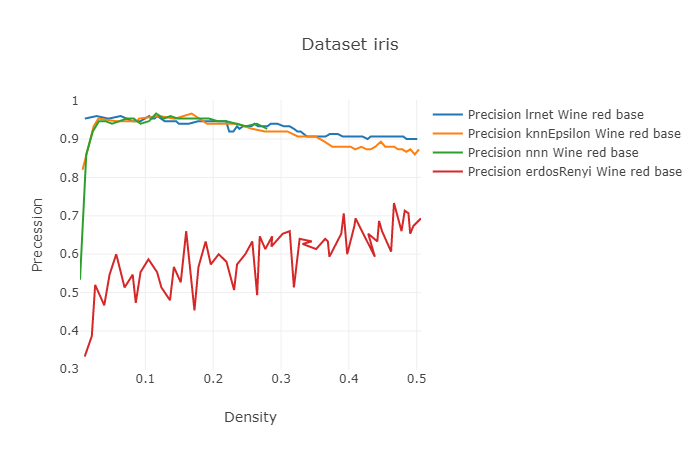
\includegraphics[width=\textwidth]{plot_iris.png}
    \caption{Vplyv hustoty siete na kvalitu zaradenia pre dataset Iris}
\end{figure} 
\begin{figure}[H]
\centering
    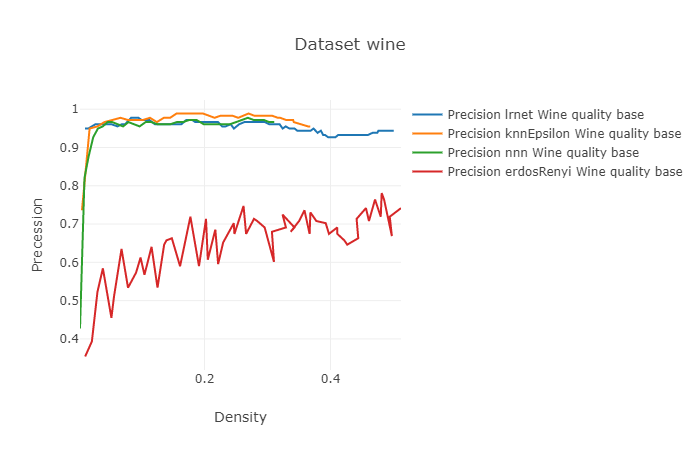
\includegraphics[width=\textwidth]{plot_wine.png}
    \caption{Vplyv hustoty siete na kvalitu zaradenia pre dataset Wine quality}
\end{figure} 
\begin{figure}[H]
\centering
    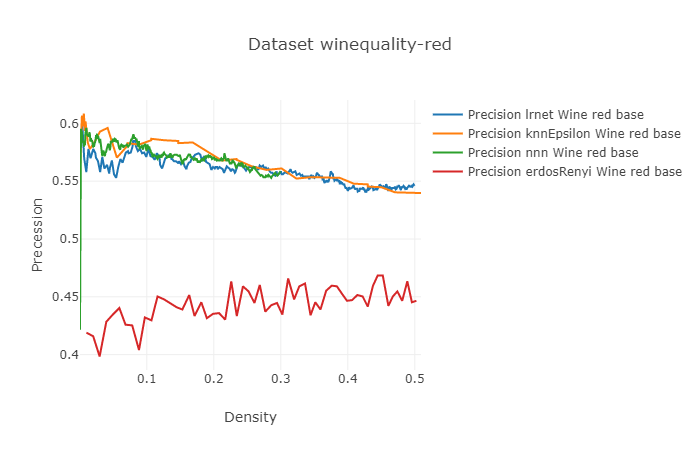
\includegraphics[width=\textwidth]{plot_wine_red.png}
    \caption{Vplyv hustoty siete na kvalitu zaradenia pre dataset Wine red}
\end{figure} 
\begin{figure}[H]
\centering
    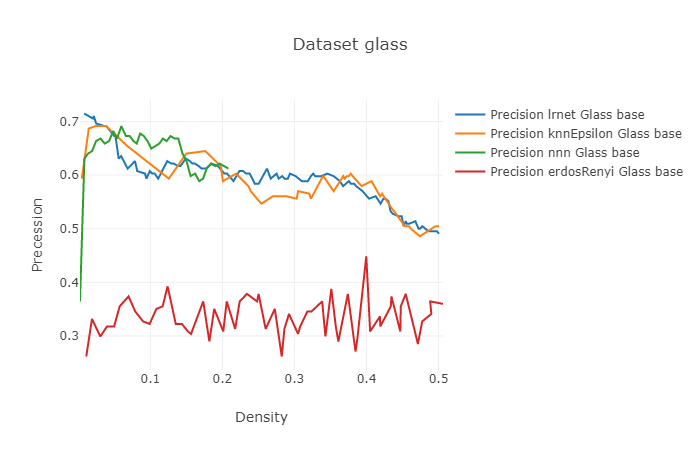
\includegraphics[width=\textwidth]{plot_glass.png}
    \caption{Vplyv hustoty siete na kvalitu zaradenia pre dataset Glass}
\end{figure} 




\end{document}
    